\documentclass[
  a4paper,
  twoside,
% oneside,
% openany,
  notitlepage,      %% Separate Titelseite (alternativ: titlepage)
  ngerman,          %% Das Dokument ist in neuen deutschen Rechtschreibung gehalten
  11pt,
% draft,            %% Finden von �berlangen Zeilen (dargestellt durch schwarze Bl�cke)
]{book}             %% Dokumentklasse (alternativ: article, report, etc.)
       
%% \linebreak f�r Zeilenumbruch
\usepackage[latin9]{inputenc}               %% Eingabezeichensatz zur Darstellung von Umlauten (latin1) erweitert um Sonderzeichen wie EURO (latin9)
\usepackage{csquotes}                       %%
\usepackage{times}                          %% Schrift Times
%\usepackage{mathpazo}                      %% Schrift Palatino
%\usepackage{luximono}                      %% Fette Schreibmaschinenschrift
\usepackage[a4paper]{geometry}              %%
\usepackage[hyphens]{url}                   %%
\usepackage{caption}
\usepackage{subcaption}                     %% Besser als subfigure und subfig
\usepackage{picins}                         %%
\usepackage{longtable}                      %%
\usepackage{shadethm}                       %%
\usepackage{amsmath}                        %%
\usepackage{framed, color}                  %%
\usepackage{fancyhdr}                       %%
\usepackage{lscape}                         %% stellenweises Querformat
\usepackage[T1]{fontenc}                    %% Europaeische Schriftcodierung (T1) und 
\usepackage{here}                           %% Grafik dort positionieren wo man es will ([H])Kopfzeile und Seitenzahlen
\usepackage[ngerman]{babel}                 %% => ngerman = neue deutsche Rechtschreibung
\usepackage{graphicx}                       %% Zur Einbindung von Grafiken. Z.B. ueber \includegraphics
\usepackage{listings}                       %% Codelistungs formatieren
\usepackage{chngpage}                       %% Seiteneinstellungen anpassen (adjustwidth)
\usepackage{paralist}                       %% flexible Listen
\usepackage{url}                            %% Darstellung von Internetadressen und Pfaden
\usepackage{setspace}                       %% zum Erzeugen von groesseren Zeilenabstaenden
\usepackage{nomencl}                        %% Abkuerzungsverzeichnis erstellen
\usepackage{tabularx}                       %% Tabellen mit fester breite nutzen
\usepackage{multirow}                       %% Zellen in Tabellen zusammenfassen
\usepackage[clearempty]{titlesec}           %% Keine Seitenzahlen, Kopf- und Fusszeilen auf leeren Seiten
\usepackage{savefnmark}                     %% Fussnoten mehrfach verwenden
\usepackage{colortbl}                       %% Farben in Tabellen
\usepackage{booktabs}                       %%
%\usepackage{hyperref}                       %% Phantomsection
\usepackage[backend=bibtex8,style=alphabetic]{biblatex}      %% "`Abgerufen am"' bei online quellen
% see styles: ftp://ftp.fu-berlin.de/tex/CTAN/macros/latex/exptl/biblatex/doc/biblatex.pdf
% default style: numeric
\usepackage{eurosym}
\usepackage{placeins}                       %% floatbarrier
\usepackage{blindtext}                      %% lorem ipsumtext
\usepackage{nomencl}                        %% Abk�rzungsverzeichnis
%\usepackage[intoc]{nomencl}                 %% Abk�rzungsverzeichnis
\usepackage{xspace}                         %% nicht erzwungene Leerzeichen (f�r \newcommand n�tzlich}
\usepackage{todo}

%\onehalfspacing                             %% 1.5 Zeilenabstand
%\doublespacing                              %% Doppelter Zeilenabstand
%%%%%%%%%%%%%%%%% links %%%%%%%%%%%%%%%%%%%%%%%%%%%%%%%%%%%%%%%%%%
\usepackage[pdftex, pdfborder={0 0 0},colorlinks, linkcolor=black, citecolor=black, filecolor=black, urlcolor=blue, bookmarks=true, bookmarksnumbered=true]{hyperref}
%%%%%%%%%%%%%%%%%%%%%%%%%%%%%%%%%%%%%%%%%%%%%%%%%%%%%%%%%%%%%%%%%%

%-------------------------------------------------------------------------
%���Listings
%-------------------------------------------------------------------------

% Einstellungen f�r Listings mit Eclipse Code Style.
\usepackage{color}
\usepackage{courier}
\definecolor{sh_comment}{rgb}{0.12, 0.38, 0.18 }     % adjusted, in Eclipse: {0.25, 0.42, 0.30 } = #3F6A4D
\definecolor{sh_keyword}{rgb}{0.37, 0.08, 0.25}      % #5F1441
\definecolor{sh_string}{rgb}{0.06, 0.10, 0.98}       % #101AF9% Farbe f�r Kommentare
\def\lstsmallmath{\leavevmode\ifmmode \scriptstyle \else� \fi}
\def\lstsmallmathend{\leavevmode\ifmmode� \else� \fi}

\newcommand{\lstJava}[1]{\lstinline[language=Java,breaklines=true,basicstyle= \listingsfontinline]$#1$}
\newcommand{\lstXML}[1]{\lstinline[language=XML,breaklines=true,basicstyle= \listingsfontinline]$#1$}

\newcommand{\lstSetTiny}{\lstset{basicstyle= \tiny\ttfamily}}
\newcommand{\lstSetNormal}{\lstset{basicstyle= \scriptsize\ttfamily}}
\newcommand{\lstSetBig}{\lstset{basicstyle= \ttfamily\mdseries}}

\newcommand{\lstSetJava}{\lstset{
  language=java,
  frame=single, %shadowbox,
  rulesepcolor=\color{black},
  showspaces=false,
	showtabs=false,
	tabsize=2,
  numberstyle=\tiny\ttfamily,
	numbers=left,
  basicstyle=\scriptsize\ttfamily,
  stringstyle=\color{sh_string},
  keywordstyle=\color{sh_keyword}\bfseries,
  commentstyle=\color{sh_comment}\itshape,
  captionpos=b,
  xleftmargin=0.7cm,
	xrightmargin=0.5cm,
  lineskip=-0.1em,
	breaklines=true,
  escapebegin={\lstsmallmath},
	escapeend={\lstsmallmathend},
	morekeywords={def, use}
}}
\newcommand{\lstSetXML}{\lstset{
  language=XML,
  frame=single, %shadowbox,
  rulesepcolor=\color{black},
  showspaces=false,
	showtabs=false,
	tabsize=2,
  numberstyle=\tiny\ttfamily,
	numbers=left,
  basicstyle=\scriptsize\ttfamily,
  stringstyle=\color{sh_string},
  keywordstyle=\color{sh_keyword}\bfseries,
  commentstyle=\color{sh_comment}\itshape,
  captionpos=b,
  xleftmargin=0.7cm,
	xrightmargin=0.5cm,
  lineskip=-0.1em,
	breaklines=true,
  escapebegin={\lstsmallmath},
	escapeend={\lstsmallmathend},
	morekeywords={encoding,xs:schema,xs:element,xs:complexType,xs:sequence,xs:attribute}
}}
\lstdefinelanguage{EBNF}{
  keywords={procedure,end,return,integer,real,foreach,for,each,
  do,if,then,else,while,until,true,false,algorithm}, 
  comment=[l]{//}
}
\newcommand{\lstSetEBNF}{\lstset{
  language=EBNF,
  frame=single, %shadowbox,
  rulesepcolor=\color{black},
  showspaces=false,
	showtabs=false,
	tabsize=2,
  numberstyle=\tiny\ttfamily,
	numbers=left,
  basicstyle=\scriptsize\ttfamily,
  stringstyle=\color{sh_string},
  keywordstyle=\color{sh_keyword}\bfseries,
  commentstyle=\color{sh_comment}\itshape,
  captionpos=b,
  xleftmargin=0.7cm,
	xrightmargin=0.5cm,
  lineskip=-0.1em,
	breaklines=true,
}}

\lstSetJava

%\usepackage{fontspec}                        %% Codelistungs formatieren
%\newfontfamily\listingsfontinline[Scale=0.8]{Courier New} 
%\newfontfamily\listingsfont[Scale=0.7]{Courier}


\bibliography{bibliography/bibliography}
\definecolor{shadecolor}{gray}{.65}
\definecolor{lightgrey}{gray}{.90}
\geometry{top=3cm, bottom=3cm, inner=4cm, outer=3cm}  %% Seitengroesse festlegen 

%%Einr�ckung bei neuem Absatz entfernen
\setlength{\parindent}{0pt}
\setlength{\parskip}\medskipamount % besser als explizite Angabe in pt

%%%%%%%%%%%%%%%%  Kopfzeile und Seitenzahlen %%%%%%%%%%%%%%%%%%%%%
\setlength{\headheight}{27pt}    %\setlength{\headheight}{15pt}
\pagestyle{fancy}
\fancypagestyle{plain}{}
\lhead{} 
\fancyfoot{}                      % Fu�zeile l�schen?
\fancyfoot[EL]{\thepage}          % Seitenzahlen rechts anzeigen auf geraden seiten
\fancyfoot[OR]{\thepage}
\renewcommand{\headrulewidth}{0pt}
%%%%%%%%%%%%%%%%%%%%%%%%%%%%%%%%%%%%%%%%%%%%%%%%%%%%%%%%%%%%%%%%%%

%%%%%%%%%%%%%%%%%%% Abk�rzungsverzeichnis %%%%%%%%%%%%%%%%%%%%%%%%
\let\abbrev\nomenclature
\renewcommand{\nomname}{Abk�rzungsverzeichnis}
\setlength{\nomlabelwidth}{.25\hsize}
\renewcommand{\nomlabel}[1]{#1 \dotfill}
\setlength{\nomitemsep}{-\parsep}
\makeindex
\makenomenclature
%%%%%%%%%%%%%%%%%%%%%%%%%%%%%%%%%%%%%%%%%%%%%%%%%%%%%%%%%%%%%%%%%%


%% Anzahl der Nummerierungsebenen festlegen
%% In der book-Klasse wird nur bis zur 3 Ueberschirftenebene
%% durchnummeriert. M�chte man weitere Ebenen hinzufuegen, so
%% muss dies hier angegeben werden. Z�hlung beginnt bei 0.
\setcounter{tocdepth}{2} % im Inhaltsverzeichnis anzeigen
\setcounter{secnumdepth}{2}

%% Hurenkinder und Schusterjungen vermeiden
\widowpenalty=10000
\clubpenalty=10000

% automatischen Zeilenumbruch verbessern
\setlength{\emergencystretch}{10em}

%farben interessant \lstset{language=Java,captionpos=b,tabsize=3,frame=lines,keywordstyle=\color{blue},commentstyle=\color{darkgreen},stringstyle=\color{red},numbers=left,numberstyle=\tiny,numbersep=5pt,breaklines=true,showstringspaces=false,basicstyle=\footnotesize,emph={label}}

%% 
%% Sollte es vorkommen das Woerter nicht korrekt getrennt werden, bzw. nur an bestimmten Stellen oder nie getrennt werden sollen,
%% so koennen diese, durch Leerzeichen getrennt, mit der richtigen Trennung (durch ein Minus dargestellt) hier angegeben werden.
\hyphenation{
}

\newcommand{\akademGradKurz}{Master}
\newcommand{\akademGrad}{\akademGradKurz~of Science}
\newcommand{\ausarbeitung}{\akademGradKurz-Arbeit}
\newcommand{\thema}{Modellierung und Generierung von Testdaten f�r Datenbank-basierte Anwendungen}
\newcommand{\abgabedatum}{11. Oktober 2013}
\newcommand{\ort}{Konstanz}
\newcommand{\studGang}{Master Informatik}

\newcommand{\geboren}{22.12.1981}
\newcommand{\geborenIn}{TODO}
\newcommand{\autor}{Nikolaus Moll}
\newcommand{\autorMatNr}{287336}
\newcommand{\autorStrasse}{TODO}
\newcommand{\autorPLZ}{TODO}
\newcommand{\autorOrt}{TODO}

\newcommand{\prueferA}{TODO}
\newcommand{\prueferATitle}{TODO}
\newcommand{\prueferAInstanz}{TODO}
\newcommand{\prueferAAdresse}{TODO}
\newcommand{\prueferAPLZ}{TODO}
\newcommand{\prueferAOrt}{TODO}

\newcommand{\prueferB}{PRUEFERB}
\newcommand{\prueferBTitle}{PRUEFERBTITLE}
\newcommand{\prueferBInstanz}{TODO}
\newcommand{\prueferBAdresse}{TODO}
\newcommand{\prueferBPLZ}{TODO}
\newcommand{\prueferBOrt}{TODO}

\newcommand{\footnoteremember}[2]{
  \footnote{#2}
  \newcounter{#1}
  \setcounter{#1}{\value{footnote}}

} \newcommand{\footnoterecall}[1]{

  \footnotemark[\value{#1}]
} 

\newcommand{\refabb}[1]{siehe Abb.~\ref{#1}}
\newcommand{\refimg}[1]{siehe Abb.~\ref{#1}}
\newcommand{\refsec}[1]{siehe Abschnitt~\ref{#1}}
\newcommand{\refchap}[1]{siehe Kapitel~\ref{#1}}
\newcommand{\reflst}[1]{siehe Listing~\ref{#1}}

\begin{document}

  %% erzeugt zunaechst roemische Seitezahlen
  %\pagenumbering{roman}
  %% bei book-Klassen steht dafuer der Befehl \frontmatter zur Verfuegung
  \frontmatter
  \begin{titlepage}

% Logo einbinden

\includegraphics[width=13cm]{images/cover/htwg_logo.pdf} \\[0.5cm]
\\[3.5cm]
\begin{center}	

	% Schriftgroesse auf maximal setzen
	\Huge{
	
		% Fettschrift mit breitem Verlauf
		\textbf{\thema} \\[9.5cm]
	}
	
%	\centering
%		\includegraphics[width=8cm]{images/cover.png} \\[3.5cm]
	
	\LARGE{
		\textbf{\autor}\\
	}
	\autorMatNr \\
		
	\LARGE{
		\ort, \abgabedatum \\[1.5cm]
	}
	
	\Huge{
		\textbf{\ausarbeitung}
	}

\end{center}

\end{titlepage}
  \newpage
  \thispagestyle{empty}~  

  \thispagestyle{empty}
{
\setlength{\parskip}{0.5cm}
        \begin{center}
        \textbf{\huge \ausarbeitung}

        \textbf{zur Erlangung des akademischen Grades}

        \textbf{\Large \akademGrad}

        \textbf{an der}

        \textbf{Hochschule Konstanz}\\
        Hochschule f�r Technik, Wirtschaft und Gestaltung

        Fakult�t Informatik\\
        Studiengang \studGang
        \end{center}
}
\begin{center}
\begin{verbatim}


\end{verbatim}
\begin{tabular}{p{3cm}p{10cm}}
\textbf{Thema:} & \textbf{\thema} \\
 & \\
 & \\
 & \\
\textbf{Verfasser:} & \autor \\
	& \autorStrasse \\
	& \autorPLZ\ \autorOrt \\
	& \\
\textbf{1. Pr�fer:} & \prueferATitle\ \prueferA \\
	& \prueferAInstanz \\
	& \prueferAAdresse \\
	& \prueferAPLZ\ \prueferAOrt \\
	& \\
\textbf{2. Pr�fer:} & \prueferBTitle\ \prueferB \\
	& \prueferBInstanz \\
	& \prueferBAdresse \\
	& \prueferBPLZ\ \prueferBOrt \\
	& \\
\textbf{Abgabedatum:} & \abgabedatum
\end{tabular}
\end{center}
  \newpage
  \thispagestyle{empty}~
  
  \chapter{Abstract}
%\addcontentsline{toc}{chapter}{Abstract (Zusammenfassung)}

\begin{center}
	\begin{tabular}{p{3cm}p{10cm}}
		\textbf{Thema:} & \thema \\
		 & \\
		\textbf{Verfasser:} & \autor \\
		 & \\
		\textbf{Betreuer:} & \prueferATitle\ \prueferA \\
		                   & \prueferBTitle\ \prueferB \\
		 & \\
		\textbf{Abgabedatum:} & \abgabedatum \\
		 & \\
		\textbf{Schlagworte:} & Modellierung von Testdaten, Beziehungen in Testdaten, Generieren von Testdaten, DSL f�r Testdaten, Datenbanktest \\
		 & \\
	\end{tabular}
\end{center}

Softwaretests haben sich als Teil der Qualit�tssicherung von Softwareprojekten etabliert.
F�r Tester ist die Modellierung von Testdaten f�r Datenbank-basierte Anwendungen allerdings
nicht immer einfach. Die Daten k�nnen aufgrund von Beziehungen von Datens�tzen schnell
un�bersichtlich und komplex werden. Wegen der Komplexit�t versuchen Tester, mehrere Tests
mit denselben Daten durchzuf�hren.

In dieser Masterarbeit werden eine neue Modellierungssprache f�r Testdaten f�r
Datenbank-basierte Anwendungen und ein Algorithmus zur Generierung von Testdaten 
vorgestellt. Die Sprache erlaubt eine �bersichtliche Beschreibung von Daten und
von Beziehungen zwischen Datens�tzen. Der Algorithmus zur Generierung erzeugt
Daten anhand der Beziehungstypen im Datenbank-Modell. Der Algorithmus versucht
viele Grenzf�lle zu erzeugen, so dass die Daten in m�glichst vielen Tests verwendet
werden k�nnen.

Die Sprache und der Algorithmus wurden implementiert und in praktischen Anwendungen
auf ihre Nutzbarkeit �berpr�ft. Die Implementierung steht unter der Open-Source-Lizenz
\textit{Apache License 2.0}.

  \newpage
  \thispagestyle{empty}~
  
  \chapter*{Ehrenw�rtliche Erkl�rung}
\addcontentsline{toc}{chapter}{Ehrenw�rtliche Erkl�rung}

Hiermit erkl�re ich
\textit{\autor,} geboren am \textit{\geboren} in \textit{\geborenIn,} dass ich\\

\begin{tabular}{lp{12cm}}
(1) & meine \ausarbeitung\ mit dem Titel \\[1em]
& \textbf{\thema} \\[1em]
& selbst�ndig und ohne fremde Hilfe angefertigt und keine anderen als die angef�hrten Hilfen benutzt habe;\\[1em]
(2) & die �bernahme w�rtlicher Zitate, von Tabellen, Zeichnungen, Bildern und
Programmen aus der Literatur oder anderen Quellen (Internet) sowie die Verwendung
der Gedanken anderer Autoren an den entsprechenden Stellen innerhalb der Arbeit
gekennzeichnet habe.\\
\end{tabular}

\vspace*{1cm}

Ich bin mir bewusst, dass eine falsche Erkl�rung rechtliche Folgen haben kann.\\

\vspace*{2cm}

\ort, \abgabedatum

\begin{verbatim}



\end{verbatim}

\begin{tabular}{c}
  \rule{5cm}{1pt}\\
  \autor\\
\end{tabular}
  \newpage
  \thispagestyle{empty}~  
  
  %% Inhaltsverzeichnis erstellen
  \cleardoublepage
  \phantomsection % n�tig damit das Inhaltsverzeichnis in selbigem korrekt verlinkt wird und keine Warnung geworfen wird
  %\addcontentsline{toc}{chapter}{Inhaltsverzeichnis}
  \tableofcontents

  %% Setzt den Seitezaehler zurueck und erzeugt ab hier arabische Seitenzahlen
  %\pagenumbering{arabic}
  %% bei book-Klassen steht dafuer der Befehl \mainmatter zur Verfuegung
  \mainmatter
  
  \chapter{Einleitung}

\todo{Einleitung schreiben}
- Motivation / allgemeine Problemstellung

- Aufgabenstelung / Zielsetzung

\subsection{Zielsetzung}

\subsection{Aufbau der Arbeit}


\todo{Weitere Quellen und Zitate einbauen}

\section*{Ungenutzte Quellen}
\begin{enumerate}
	\item \cite[20ff]{DER_INTEGRATIONSTEST}
	\item \cite{MODELLGETRIEBENE_SOFTWAREENTWICKLUNG}
	\item \cite{DOMAIN_DRIVEN_DESIGN}
\end{enumerate}

  \chapter{Grundlegende Konzepte}
\label{chap:grundlagen}

noch zu erkl�ren:
- benutzte Terminologie
- Modellgetriebene Software-Entwicklung
- Tests, Testdatengenerierung
- Literatur nutzen



\section{Modellgetriebene Software-Entwicklung}


\begin{itemize}
	\item \textbf{M0}: Konkrete Information
	\item \textbf{M1}: Meta-Daten zum Beschreiben der Information. Auch als \textit{Modell} bezeichnet.
	\item \textbf{M2}: 
	\item \textbf{M3}:
\end{itemize}

- Modell, Meta-Modell, Modell-Ebenen
- http://www.omg.org/spec/MOF/ISO/19502/PDF/ spricht von den klassischen 4 schichten...
- DSL, intern vs. extern



\section{Software-Tests}
\label{sec:grundlagen:konzepte:tests}

\nomenclature{SUT}{System Under Test (\refsec{sec:grundlagen:konzepte:tests})}
Eine zu pr�fende Anwendung wird im Kontext von Software-Tests als \textit{System Under Test} (abgek�rzt SUT) bezeichnet.
Dabei bezeichnet SUT je nach Test Klassen, Objekte, Methoden oder vollst�ndige Anwendungen. 
\cite[810f]{XUNIT_TEST_PATTERNS}

Alle Voraussetzungen und Vorbedingungen f�r einen Test werden unter der Bezeichnung \textit{Test Fixture} zusammengefasst.
Ein Test Fixture repr�sentiert den Zustand des SUT vor den Tests. \cite[814]{XUNIT_TEST_PATTERNS} Es gibt verschiedene
Arten von Test Fixtures. Folgende zwei Test Fixtures sind f�r diese Arbeit relevant:

\begin{itemize}
	\item \textbf{Standard Fixture}: Ein Test Fixture wird als Standard Fixture bezeichnet, wenn es f�r alle bzw. fast alle 
	  Tests verwendet werden kann. Ein Standard Feature reduziert nicht nur den Aufwand zum Entwerfen von Testdaten f�r die
		einzelnen Tests, sondern verhindert dar�ber hinaus, dass der Test-Ingenieur  sich bei verschiedenen Tests immer wieder
		in unterschiedliche Test-Daten hineinversetzen muss. Nur in Ausnahmef�llen sollten Tests modifizierte oder eigene 
		Testdaten verwenden. \cite[305]{XUNIT_TEST_PATTERNS}
	
	\item \textbf{Minimal Fixture}: Minimal Fixtures stellen Test Fixtures dar, deren Umfang auf ein Minimum reduziert wurde. 
	  Dadurch lassen sich Minimal Fixture im Allgemeinen leichter verstehen. Das Reduzieren der Daten kann auch zu
		Leistungsvorteilen bei der Ausf�hrung der Tests f�hren. \cite[302]{XUNIT_TEST_PATTERNS}
\end{itemize}



Eine �bliches Muster, Systeme in Verbindung mit Datenbanken zu testen, ist \textit{Back Door Manipulation}.
Dabei wird die Datenbank �ber direkten Zugriff, vorbei am zu testenden System, in den Anfangszustand gebracht.
Anschlie�end k�nnen die zu testenden Operationen am System durchgef�hrt werden. Um zu �berpr�fen, ob sich das System richtig
verhalten hat, wird der Zustand der Datenbank mit dem erwarteten Zustand verglichen - ebenfalls am zu testenden System vorbei.
\cite[327ff]{XUNIT_TEST_PATTERNS}

\todo{Grafik Back Door Manipulation}

Es gibt mehrere Vorteile, die Datenbank nicht �ber das zu testende System in den Anfangszustand zu bringen. Einerseits k�nnen
semantische Fehler im zu testenden System unter Umst�nden nur so gefunden werden. Andererseits kann der Zustand mitunter
schneller in die Datenbank geschrieben werden, wenn nicht der Weg �ber das zu testende System gemacht wird. Au�erdem bietet es
in Bezug auf die Zust�nde eine h�here Flexibilit�t: Die Datenbank kann auch in Zust�nde	gebracht werden, die �ber das System
nicht erreicht werden k�nnen. Daf�r leidet die Flexibilit�t an einer anderen Stelle: Die Tests sind abh�ngig vom konkret
verwendeten Datenbank-System. Wird die Datenbank von SQL auf NoSQL umgestellt, m�ssen die Tests angepasst werden. 
Au�erdem setzt der direkte Zugriff auf die Datenbank voraus, dass die Semantik der
zu testenden Anwendung ber�cksichtigt wird. Aus Sicht der Anwendung d�rfen sich von der Anwendung eingespielte Daten in ihrer
Form nicht von den manuell in die Datenbank geschriebenen Daten unterscheiden.

\todo{Layer test erkl�ren}


\section{DbUnit}

\todo{DataSets erkl�ren}




\section{SB Testing DB}
\label{sec:grundlagen:sbtestingdb}

Die Firma SEITENBAU verwendet f�r die Java-basierten Datenbankanwendungen das Framework JUnit mit der Erweiterung DbUnit. Da
die Modellierung der Testdaten mit DbUnit-eigenen Mitteln einige Nachteile hat (siehe Abschnitt \ref{sec:fragestellung:modellierung}), hat SEITENBAU die Bibliothek \textit{SB Testing DB} entwickelt.  \textit{SB Testing DB} generiert anhand eines Dom�nen-spezifischen
Datenbank-Modells ein individuelle Klassen zur Modellierung von Testdaten.

Die generierten Klassen setzen das Builder-Pattern (\cite[11ff]{EFFECTIVEJAVA2ND}) mit einem Fluent API
(\cite[68ff]{DOMAIN_SPECIFIC_LANGUAGES}) um. In Java werden Fluant APIs mit Hilfe von Method Chaining verwirklicht. Dabei
liefern Modifikator-Methoden wie Setter das Host-Objekt selbst zur�ck. Das erlaubt es, mehrere Modifikationen auf dem selben
Objekt  mit nur einem Ausdruck durchzuf�hren \cite[373f]{DOMAIN_SPECIFIC_LANGUAGES}. Die Nutzung k�nnte so aussehen:
\texttt{student.name("Moll").vorname("Nikolaus")}.

Abbildung \ref{img:sbtestingmodel} stellt grafisch dar, wie aus einem Datenbank-Modell das Fluent API erzeugt wird. Ausgangspunkt ist
ein relationales Datenbankmodell. Dieses Modell muss in ein f�r den Generator interpretierbares Modell, das das SB-Testing-DB-Modell,
transformiert werden. Dies kann automatisch (z.B. wenn das Modell in Form eines \textit{Apache-Torque}-Modell vorliegt) oder manuell
geschehen. Das SB-Testing-DB-Modell enth�lt Informationen zu Tabellennamen und Angaben zu den Spalten, z.B. Namen und Datentypen. 

\begin{figure}[H]
	\centering
	 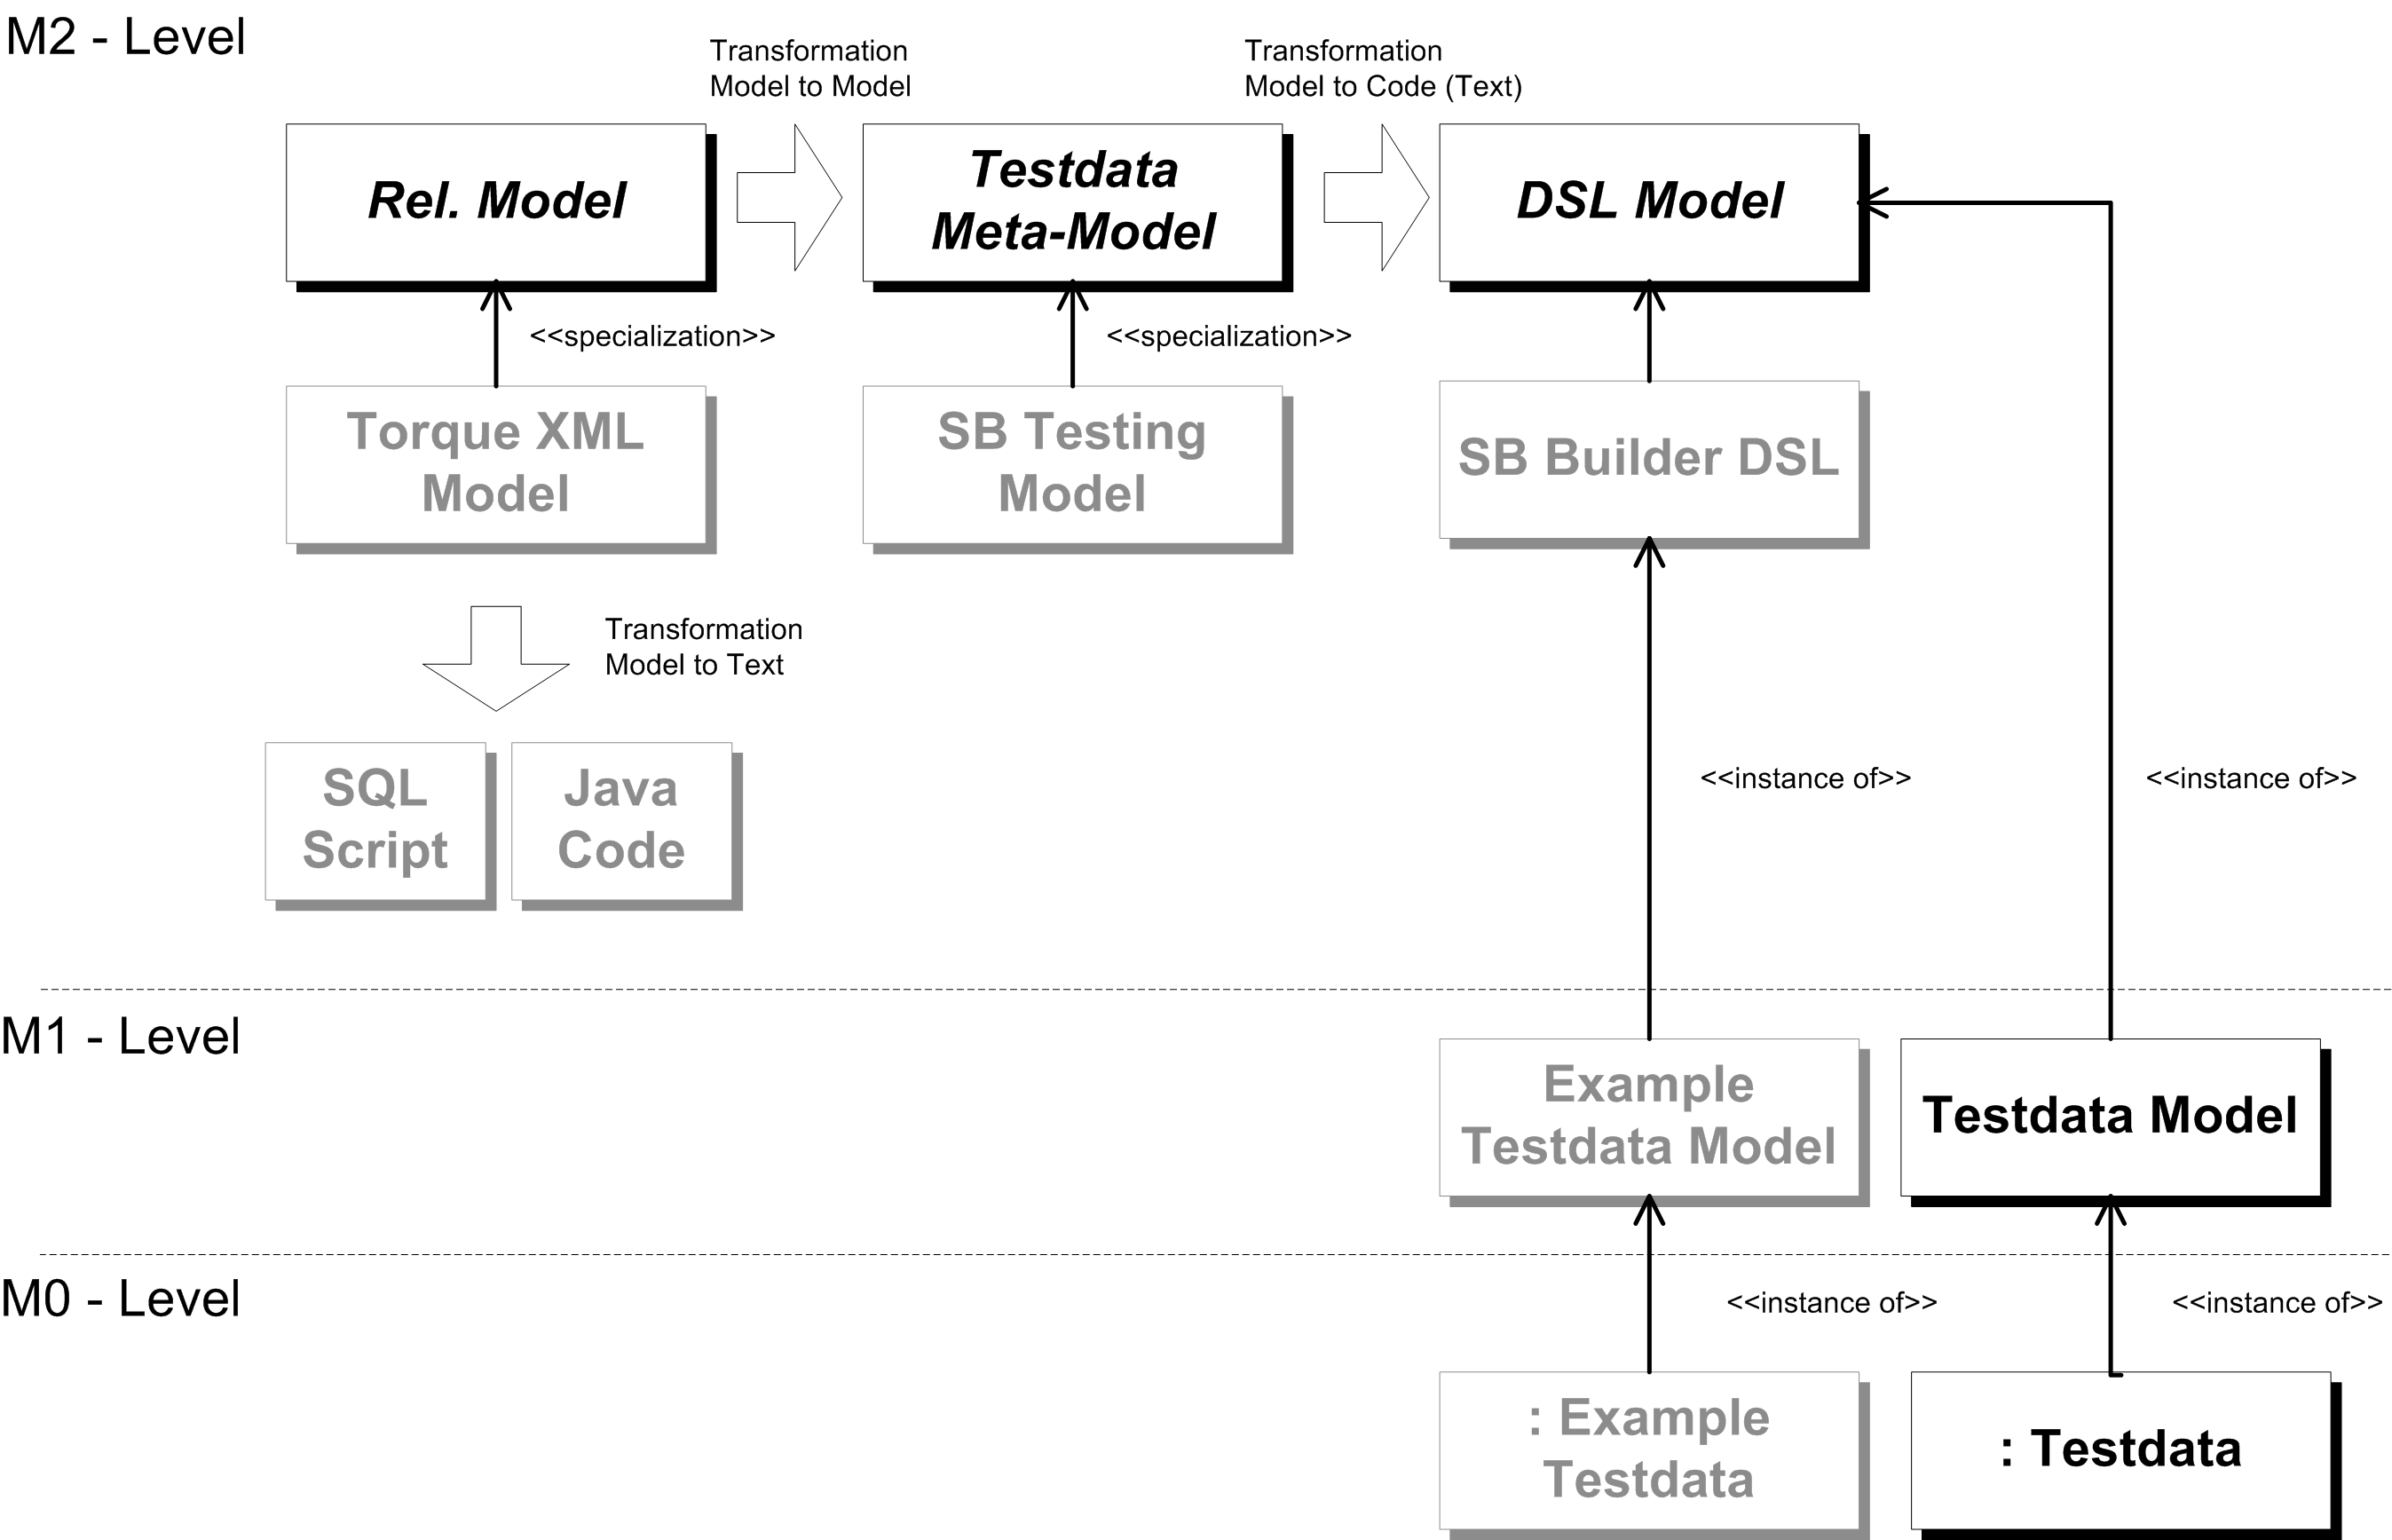
\includegraphics[width=0.95\textwidth]{images/grundlagen/sb_testing_model.png}
	\caption{Modell-Beschreibung}\label{img:sbtestingmodel}
\end{figure}

Das SB-Testing-DB-Modell enth�lt keine Datenbank-Constraints. Eine Abbildung dieser w�rde keine wesentliche Vorteile bringen. Das API
bzw. die erzeugten DataSets sind ausschlie�lich f�r den Einsatz im Test-Umfeld gedacht. Sollte ein DataSet Daten enthalten, die gegen 
die in der Datenbank definierten Constraints versto�en, scheitert das Einspielen des DataSets in die Datenbank und eine Fehlermeldung
wird ausgel�st.
Aus Sicht des Testers ist dieses Verhalten ausreichend, da die Exception zum Scheitern der Unit-Tests f�hren wird. Der Mehrwert,
dass ung�ltige DataSets schon vor dem Einspielen als solches zu erkennen, ist gering im Vergleich zu dem Aufwand, 
Constraint-Mechanismen verschiedener Datenbanksysteme nachzubauen.

Der Generator nutzt f�r die Code-Generierung \textit{Apache Velocity}. Velocity ist eine Template-Engine, die Dokumente mit Hilfe von
Templates erzeugt. Diese Templates bestehen aus Text und besonderen Velocity-Anweisungen. Zu den Anweisungen geh�ren unter anderem
Platzhalter, die w�hrend der Generierung durch konkrete Werte ausgetauscht werden. Velocity bietet mit Verzweigungen und Schleifen
auch Anweisungen zur Steuerung der Generierung.

Templates Dokumente erzeugt. Die Vorlagen k�nnen Platzhalter enthalten, die von Velocity durch konkrete Werte ausgetauscht werden, und
auch von Velocity interpretierte Steueranweisungen, z.B. Verzweigungen und Schleifen.



Die Namen der generierten Klassen h�ngen vom Modell ab. Unter anderem werden Klassen der folgenden Kategorien erzeugt:
\begin{itemize}

	\item \textbf{DataSet}: Es wird eine abstrakte DataSet-Klasse generiert. Der Zugriff auf die Tabellen erfolgt �ber �ffentliche
	  Felder. Die Klasse enth�lt die Methode \texttt{createDBUnitDataSet}, um die f�r die Unit-Tests ben�tigten DbUnit-DataSets zu
		erzeugen. Dabei werden Template-Methoden definiert, die genutzt werden k�nnen, um in den Erzeugungsprozess von DataSets
		einzugreifen. Die Klasse enth�lt dar�ber hinaus Methoden zum Hinzuf�gen von Zeilen in die entsprechende
		Tabellen.

	\item \textbf{Table}: F�r jede Tabelle wird eine entsprechende Klasse generiert. Der Klassenname setzt sich aus dem Namen
	  der Tabelle und dem Suffix "`Table"' zusammen. Die Klasse stellt Methoden zum Modellieren der Daten und f�r den Zugriff
		auf Tabellenzeilen bereit. 
		Einzelne Tabellenzeilen werden von einer passenden RowBuilder-Klasse repr�sentiert.
		Damit die Klasse direkt zur Erstellung von DbUnit-DataSets verwendet werden kann, implementiert sie das DbUnit-Interface
		\texttt{ITable}.
	
	\item \textbf{RowBuilder}: Zu jeder Tabelle wird eine Klasse zur Repr�sentation einer Tabellenzeile generiert. Die Klasse
	  beinhaltet f�r jede Spalte mehrere Methoden zum Setzen und Abfragen des jeweiligen Wertes. Die Methodennamen setzen sich
		zusammen aus der Aufgabe (\texttt{get} bzw. \texttt{set}) und dem Spaltennamen. \todo{Raw-Setter erkl�ren?}
	
	\item \textbf{FindWhere}: F�r einfache Suchanfragen gibt es f�r jede Tabelle die innere Klasse \texttt{FindWhere}. Sie erm�glicht
	  die Suche nach  einem Wert in einer Spalte und liefert eine Liste von Tabellenzeilen. Die Methode ist zur Suche nach Zeilen
		vorgesehen, von denen erwartet wird, dass es sie gibt. Passt keine Zeile zum Suchkriterium gefunden, wird eine
		Exception ausgel�st.
	
\end{itemize}

\todo{Bild mit Text integrieren}

\begin{figure}[H]
  \centering
	 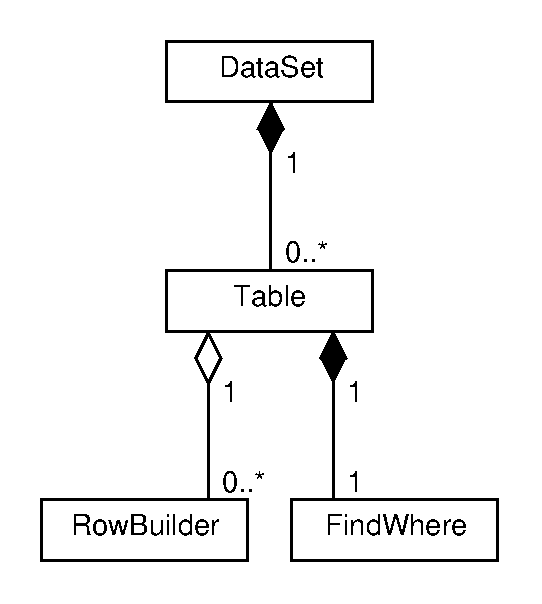
\includegraphics[width=0.4\textwidth]{images/grundlagen/sb_testing_classes.pdf}
	\caption{UML-Klassendiagramm der SB Testing DataSet Klassen}\label{img:sb_testing_classes}
\end{figure}




\section{Konventionen}
\label{sec:grundlagen:konventionen}

	\subsection{Datenbank ER-Diagramme}
	\label{sec:grundlagen:konventionen:datenbankdiagramme}
	F�r die Darstellung von Datenbank-Diagrammen wird ein einheitlicher Stil verwendet. Dieser orientiert sich an
	Ambler aus \cite{REFACTORING_DATABASES}. Auf die Angabe von Stereotypen wird sowohl bei den Tabellen, als auch
	bei den Beziehungen zwischen Tabellen verzichtet.
	
	Erkl�ren:
	- Spalten/PK/FK
	- Kardinalit�ten
	
	- basiert auf UML, Stereotypen bei Tabelle und Beziehungen weggelassen, 
	
	Abbildung \ref{img:ambler_table} zeigt ein Diagramm mit zwei Tabellen. Tabelle 2 enth�lt einen Fremdschl�ssel,
	der einem Prim�rschl�ssel aus Tabelle 1 

	\begin{figure}[H]
		\centering
		 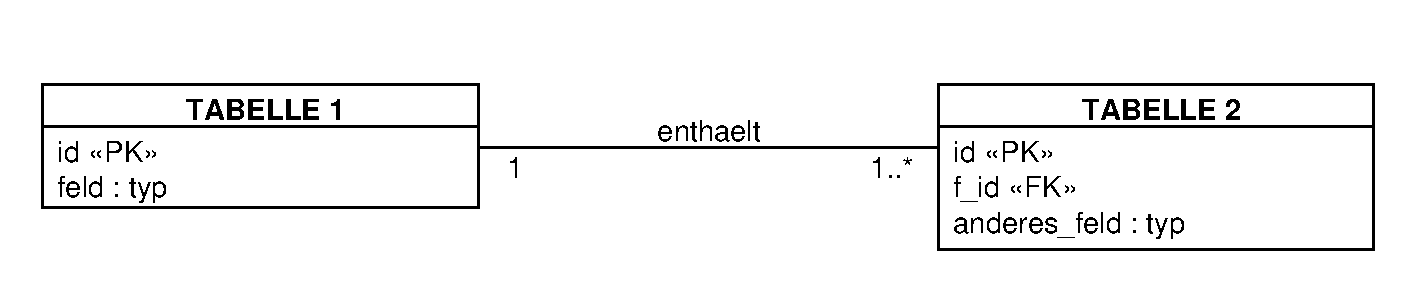
\includegraphics[width=0.75\textwidth]{images/grundlagen/ambler_table.pdf}
		\caption{Datenbank-Diagramm-Stil nach Ambler}\label{img:ambler_table}
	\end{figure}


  \chapter{Anforderungsanalyse / Fragestellung}
\label{chap:anforderungen}

Einleiten: Zwei Fragestellungen, DSL und Generierung

\section{Allgemeine Anforderungen}
\label{sec:anforderungen:allgemeineanforderungen}

Die Hauptziele dieser Arbeit stellen sich wie folgt dar:
\begin{enumerate}
	\item Vereinfachen der Modellierung von Beziehungen
	\item Modellierung von Test-Daten �bersichtlicher machen
	\item Automatisches Generieren von Test-Daten
\end{enumerate}


F�r die Modellierung gelten diese allgemeinen Anforderungen:

\begin{itemize}
	\item \textbf{Integration in bestehende Werkzeugkette}: Die L�sung sollte sich nach M�glichkeit in die bestehende
	  Werkzeugkette von SEITENBAU integrieren lassen.  
		
  \item \textbf{IDE-Integration}: Bedienbarkeit f�r den Tester stellt eine der wichtigsten Anforderungen dar. Daten sollen
	  komfortabel modelliert werden k�nnen. Die Integration in Entwicklungsumgebungen wie Eclipse oder IntelliJ IDEA muss
		gegeben sein. 
	
	\item \textbf{Beziehungen}: Beziehungen sollen einfach modellieren werden k�nnen. 

	\item \textbf{G�ltigkeitsbereiche}:
	  \todo{G�ltigkeitsbereiche erkl�ren}

	\item \textbf{Ver�nderbarkeit von DataSets}: DataSets sollen sich bei der Modellierung beliebig ver�ndern lassen.
	
	\item \textbf{Komposition}: DataSets sollen sich aus anderen DataSets zusammensetzen lassen.
	
	
	\item \textbf{Typ-Sicherheit}: Die Beschreibung der Daten sollte typsicher erfolgen. Idealerweise sollten falsche
	  Typen schon w�hrend des Compilierns erkannt werden.
		
	\item \textbf{Funktionen als Werte}: Es soll m�glich sein, Hilfsfunktionen zur Berechnung von Werten zu verwenden,
	  z.B. zum Einlesen von Binary Large Objects (BLOBs) aus Dateien.
		
	\item \textbf{Zielgruppe}: Die Zielgruppe f�r die DSL sind Software-Entwickler und Tester. Der Code zur Modellierung
	  der Daten sollte auch f�r andere Projekt-Mitglieder lesbar und verst�ndlich sein.

	\item \textbf{Ung�ltige Daten}: Es sollen sich auch aus Sicht der Datenbank oder des SUT ung�ltige Daten modellieren lassen.

\end{itemize}


F�r die Generierung der Testdaten lassen sich die Anforderungen folgenderma�en zusammenfassen:
\begin{itemize}
  
	\item \textbf{Fokus auf Beziehungen}: 
	
	\item \textbf{Datenmenge selbst bestimmen}:

	\item \textbf{Deterministische Generierung}: Auch wenn die Test-Daten aus Zufallsdaten bestehen, sollen sie deterministisch
	  generiert werden k�nnen. Das hei�t, dass die Generierung des Modells mit den selben Einstellungen auch zum selben Ergebnis
		f�hrt.
		
	\item \textbf{Kompatibilit�t}: Die Generierung der Testdaten soll in unterschiedliche Ausgabe-Formen erfolgen k�nnen,
	  z.B. in einer DSL, in XML oder auch in SQL-Statements.
	
\end{itemize}


\section{Modellierungskonzepte f�r Beziehungen}
\label{sec:fragestellung:modellierungskonzepte}
	
Je nach Beziehungsart gibt es unterschiedliche Ans�tze, wie diese in einem ER-Diagramm umgesetzt werden k�nnen.
Dabei k�nnen neben den Entit�ten auch die Beziehungen selbst Attribute haben.
Die folgenden drei grunds�tzlichen Beziehungsarten werden dabei unterschieden:

	\subsection{1:1-Beziehungen}
	\label{sec:fragestellung:onetoone}
	
	Eine bin�re Beziehung zwischen zwei Entit�tstypen, wobei jede Entit�t innerhalb dieser Beziehung maximal einer
	anderen Entit�t zugeordnet sein kann. Eine solche Beziehung kann realisiert werden, indem eine Tabelle um einen
	Fremdschl�ssel auf die andere erweitert wird. Dabei sollte der Fremdschl�ssel und auch die beziehungsbeschreibenden
	Attribute immer der Tabelle hinzugef�gt werden, deren Entit�ten eine Beziehung voraussetzt.
	
	Wenn viele Beziehungsattribute vorhanden sind oder die Beziehung auf beiden Seiten optional ist,
	kann es auch sinnvoll sein, eine 1:1-Beziehung wie eine n:m-Beziehung zu modellieren.

	\subsection{1:n-Beziehungen}
	\label{sec:fragestellung:onetomany}

	Eine bin�re Beziehung zwischen zwei Entit�tstypen, wobei jede Entit�t des einen Typs in Beziehung mit mehreren
	Entit�ten des anderen Typs stehen kann. Diese Entit�ten k�nnen auch nur mit maximal einer Entit�t in Beziehung
	stehen. Es ist m�glich festzulegen, wie viele Beziehungen eine Entit�t mindestens und h�chstens haben darf.
	
	Die Tabelle der Entit�ten, die maximal einer andere Entit�t zugeordnet sind, wird um einen Fremdschl�ssel
	und um f�r jede Beziehung individueller Attribute erweitert. Die Beziehungsattribute, die f�r alle Beziehungen
	der beteiligten Entit�t gelten, werden ihrer Tabelle hinzugef�gt.
	
	\subsection{n:m-Beziehungen}
	\label{sec:fragestellung:manytomany}
	
	Eine bin�re Beziehung zwischen zwei Entit�tstypen, wobei jede Entit�t des einen Typs mit mehreren Entit�ten
	des anderen Typs in Beziehung stehen kann -- und umgekehrt. Es ist m�glich, untere und obere Grenzwerte f�r
	die Anzahl der Beziehungen auf beiden Seiten festzulegen. Solche als assoziativ bezeichneten Beziehungen
	werden �ber eine Hilfstabelle modelliert, die entsprechend assoziative Tabelle genannt wird. Diese besteht
	aus den beiden Fremdschl�sseln auf die beteiligten Tabellen und den beziehungsbeschreibenden Attributen.
	
	Grunds�tzlich k�nnen assoziative Tabellen f�r alle bin�ren Beziehungen verwendet werden. Vor allem wenn 
	die Beziehung viele Attribute enth�lt, kann eine assoziative Tabelle f�r �bersichtlichere Tabellenstrukturen
	sorgen.  

	\subsection{Andere Beziehungen}
	\label{sec:fragestellung:anderebeziehungen}
	
	In der aktuellen \textit{STU}-Implementierung m�ssen andere Beziehungen manuell umgesetzt werden. Dies gilt
	auch f�r zirkul�re und reflexive, sowie alle nicht-bin�ren Beziehungen.



\section{Fortlaufendes Beispiel}
\label{sec:fragestellung:beispiel}

% Beispiel einleiten
Ein einheitliches fortlaufendes Beispiel soll der Arbeit als Grundlage dienen. Die Problemstellung besteht aus
einem Modell und einer Menge von Testdaten. Diese Testdaten dienen als Grundlage f�r die Diskussion der unterschiedlichen
Modellierungsvarianten.

	\subsection{Anforderungen an das Beispiel}
	\label{sec:fragestellung:beispiel:voraussetzungen}

	Der Schwerpunkt der Modellierung liegt bei der Darstellung von Beziehungstypen zwischen Entit�tstypen. Dabei soll die
	Problemstellung einerseits nicht zu komplex sein, damit sie �berschaubar bleibt. Andererseits soll sie komplex genug
	sein, um m�glichst alle Beziehungsarten zwischen Entit�ten abzudecken.
	Die Testdaten sollten gleichzeitig ein \textit{Standard Fixture} und ein \textit{Minimal Fixture} darstellen
	(\refsec{sec:grundlagen:konzepte:tests}).
	

	\subsection{Gew�hlte Problemstellung}
	\label{sec:fragestellung:beispiel:gewaehlte_problemstellung}
	Das gew�hlte Beispiel stellt eine starke Vereinfachung des Pr�fungswesens an Hochschulen dar. Auf eine praxisnahe
	Umsetzung wird zugunsten der Komplexit�t verzichtet. Personenbezogene Begriffe werden in der maskulinen Form verwendet,
	ohne dabei Aussagen �ber das Geschlecht der repr�sentierter Personen zu machen. Es beinhaltet die folgenden vier 
	Entit�tstypen:

	\begin{itemize}
		\item \textbf{Professor}: Ein Professor leitet Lehrveranstaltungen.
		\item \textbf{Lehrveranstaltung}: Eine Lehrveranstaltung wird von einem Professor geleitet. Es kann zu jeder
			Lehrveranstaltung eine Pr�fung geben.
		\item \textbf{Pr�fung}: Eine Pr�fung ist einer Lehrveranstaltung zugeordnet. Au�erdem hat mindestens ein Professor
			Aufsicht.
		\item \textbf{Student}: Studenten k�nnen an Lehrveranstaltungen und an Pr�fungen teilnehmen. Studenten haben au�erdem 
			die M�glichkeit, Tutoren von Lehrveranstaltungen zu sein.
		\item \textbf{Raum}: Ein Professor kann einen Raum als B�ro zugewiesen bekommen.
	\end{itemize}
	
	Die Beziehungen der Entit�tstypen stellen sich wie folgt dar: 
	\begin{itemize}
		\item \textbf{leitet}: Eine Lehrveranstaltung muss von genau einem Professor geleitet werden, ein Professor kann beliebig viele
		  oder keine Lehrveranstaltungen leiten.
		\item \textbf{gepr�ft}: Eine Pr�fung ist genau einer Lehrveranstaltung zugeordnet. Eine Lehrveranstaltung kann mehrere Pr�fungen 
		  haben (z.B. Nachschreibpr�fung).
		\item \textbf{beaufsichtigt}: Eine Pr�fung muss mindestens von einem Professor beaufsichtigt werden, ein Professor kann in 
		  beliebig vielen Pr�fungen Aufsicht haben. 
		\item \textbf{besucht}: Jeder Student kann beliebig vielen Lehrveranstaltungen besuchen. Lehrveranstaltungen ben�tigen jedoch 
		  mindestens drei Besucher um stattzufinden und sind aus Kapazit�tsgr�nden auf 100 Teilnehmer begrenzt.
		\item \textbf{ist Tutor}: Jeder Student kann bei beliebig vielen Lehrveranstaltungen Tutor sein und jede Lehrveranstaltung
			kann beliebig viele Tutoren haben. 
		\item \textbf{schreibt}: Jeder	Student kann an beliebig vielen Pr�fungen teilnehmen und umgekehrt eine Pr�fung von einer
		  beliebigen Anzahl von Studenten geschrieben werden.
		\item \textbf{hat B�ro}: Jeder Professor hat ein B�ro. Ein Raum kann einem oder keinem Professor zugeordnet sein.
	\end{itemize}

	Abbildung \ref{img:example_er} zeigt das Beispiel grafisch in Form eines ER-Diagramms. Den verschiedenen Entit�tstypen
	werden dabei Attribute zugeordnet. 
	
	\begin{figure}[H]
		\centering
		 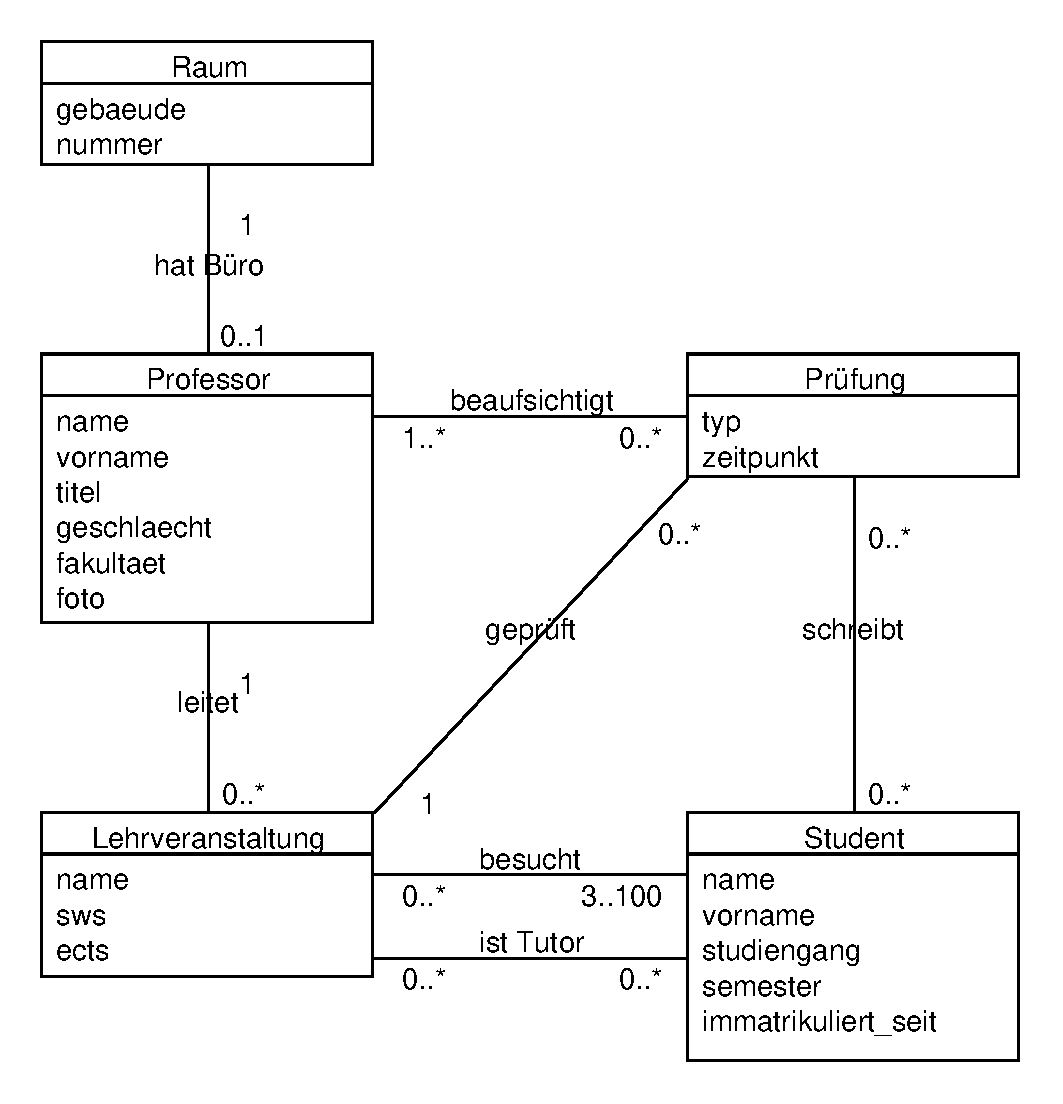
\includegraphics[width=0.65\textwidth]{images/fragestellung/example_hochschule_er.pdf}
		\caption{ER-Diagramm des fortlaufenden Beispiels}\label{img:example_er}
	\end{figure}

	Das entsprechende relationale Datenbank-Diagramm wird in Abbildung \ref{img:example_relational} dargestellt. 
	
	\begin{figure}[H]
		\centering
		 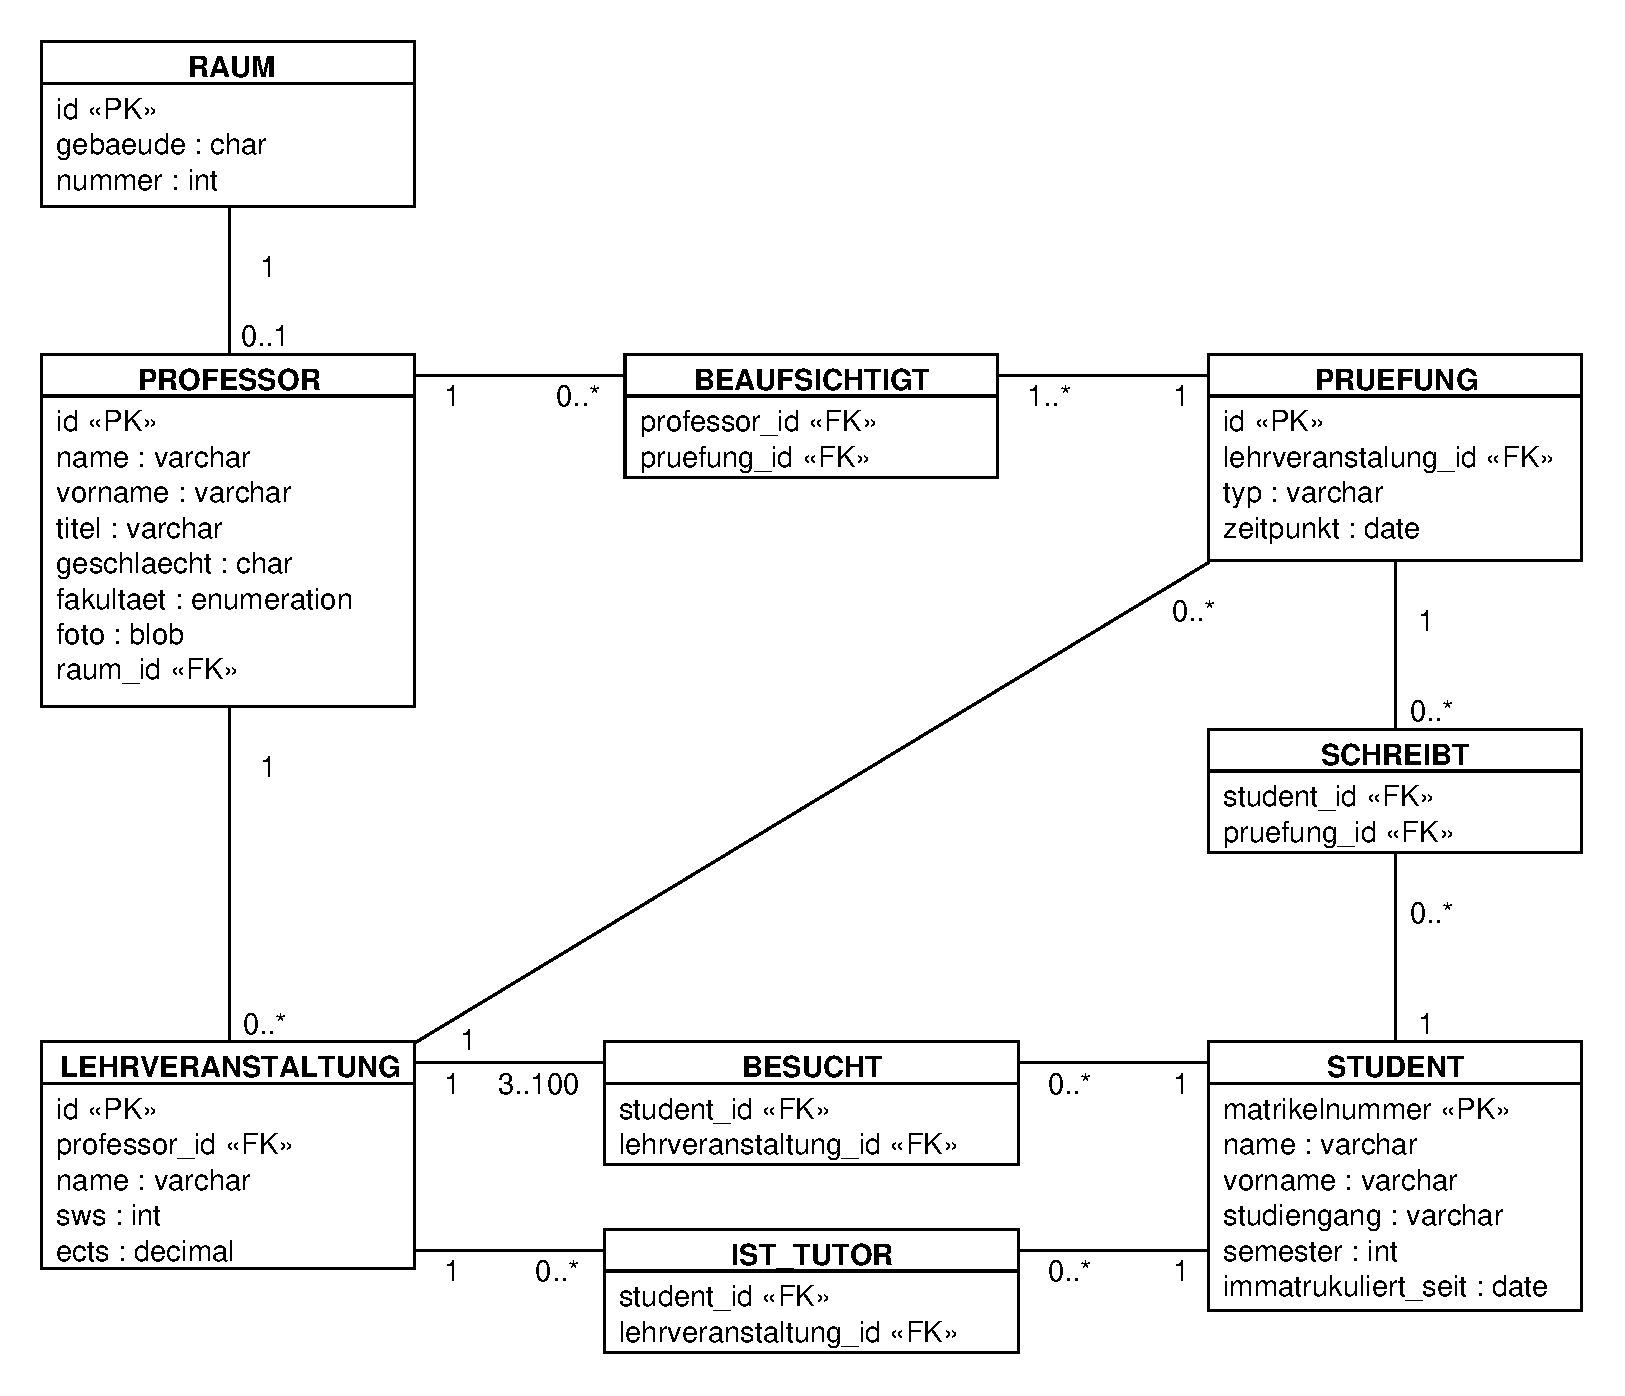
\includegraphics[width=0.95\textwidth]{images/fragestellung/example_hochschule_relational.pdf}
		\caption{Relationales Datenbank-Diagramm des fortlaufenden Beispiels}\label{img:example_relational}
	\end{figure}

	Das Attribut "`fakultaet"' in der Tabelle Professor soll als Aufz�hlungstyp (enumeration) realisiert werden.
	M�gliche Werte sind: Architektur, Bauingenieurwesen, Elektrotechnik, Informatik, Maschinenbau und Wirtschaftswesen.
	Das Foto des Professors wird als BLOB dargestellt.
	\nomenclature{BLOB}{Binary Large Object)}
	

	\subsection{Beispiel-Use-Cases}
	\label{sec:fragestellung:beispiel:usecases}

	Um den einen Kompromiss f�r die Komplexit�t der Testdaten zu finden, werden vier Fragestellungen definiert. Diese
	Fragen sollen dabei helfen, den Umfang der Testdaten bestimmen zu k�nnen. Die Fragen stellen sich wie folgt dar:

	\begin{enumerate}
		\item Welcher Professor unterrichtet die meisten Studenten?
		\item Welcher Student nimmt an den meisten Pr�fungen teil?
		\item Welcher Student ist Tutor und nimmt gleichzeitig an der Pr�fung teil?
		\item Welcher Professor macht die wenigste Aufsicht in Fremdveranstaltungen (Lehrveranstaltungen eines anderen
			Professors)?
	\end{enumerate}


\todo{�berleitung}


\section{Modellierungsvarianten der Testdaten f�r DbUnit}
\label{sec:fragestellung:modellierung}
	
	In \textit{DbUnit} werden die Datenbankzust�nde durch DataSets repr�sentiert. F�r einen Test werden gew�hnlich zwei
	DataSets ben�tigt: das erste f�r den Anfangszustand, das zweite f�r den erwarteten Zustand. Allerdings bieten
	DbUnit-DataSets nur begrenzte M�glichkeiten, das DataSet mit dem erwarteten Zustand aus dem DataSet mit dem
	Anfangszustand zu erzeugen.

	Im Folgenden werden verschiedene Modellierungsarten f�r DbUnit-DataSets diskutiert. Diese soll anhand der im
	n�chsten Abschnitt beschriebenen Kritieren erfolgen. Die Ergebnisse stellen die Grundlage
	f�r die konkretere Zielsetzung dar.

	\subsection{Kriterien f�r Bewertung}
	\label{sec:fragestellung:modellierung:sprachkriterien}

	\begin{itemize}

		\item \textbf{Zeilen}: Die Anzahl der Zeilen, die f�r ein DataSet ben�tigt werden. 
		
		\item \textbf{Zeichen pro Zeile}: Ist die Sprache f�r die Darstellung auf Bildschirmen geeignet?
		
		\item \textbf{Typsicherheit}:
		
		\item \textbf{Redundanz}: 

		\item \textbf{Benutzbarkeit (Verst�ndlichkeit und Erlernbarkeit)}:
		
		\item \textbf{Modifizierbarkeit}:

	% http://de.wikipedia.org/wiki/ISO/IEC_9126	

	\end{itemize}


	\subsection{XML-DataSet}
	\label{sec:fragestellung:modellierung:xml}
	
	Eine M�glichkeit, ein DataSet f�r DbUnit zu modellieren, stellt XML dar. DbUnit selbst bietet zwei Varianten an, DataSets
	�ber XML zu modellieren.
	
	Die erste Variante stellt das \textit{XmlDataSet} dar. Diese Klasse liest eine XML-Datei nach einem von DbUnit
	vorgegebenen Dokumententyp ein. Das Listing \ref{listing:xmldataset} zeigt einen Ausschnitt einer solchen XML-Datei,
	in dem die beiden Tabellen \textit{Professor} und \textit{Lehrveranstaltung} definiert werden.
	
	\lstSetXML
	\begin{lstlisting}[caption=XML-DataSet, label=listing:xmldataset]
<!DOCTYPE dataset SYSTEM "dataset.dtd">
<dataset>
    <table name="PROFESSOR">
        <column>id</column>
        <column>name</column>
        <column>vorname</column>
        <column>titel</column>
        <column>fakultaet</column>
        <row>
            <value>1</value>
            <value>W�sch</value>
            <value>J�rgen</value>
            <value>Prof. Dr.-Ing.</value>
            <value>Informatik</value>
        </row>
        <row>
            <value>2</value>
            <value>Haase</value>
            <value>Oliver</value>
            <value>Prof. Dr.</value>
            <value>Informatik</value>
        </row>
    </table>
    <table name="LEHRVERANSTALTUNG">
        <column>id</column>
        <column>professor_id</column>
        <column>name</column>
        <column>sws</column>
        <column>ects</column>
        <row>
            <value>1</value>
            <value>2</value>
            <value>Verteilte Systeme</value>
            <value>4</value>
            <value>5</value>
        </row>
        <row>
            <value>2</value>
            <value>2</value>
            <value>Design Patterns</value>
            <value>4</value>
            <value>3</value>
        </row>
    </table>
	...
</dataset>
	\end{lstlisting}
	
	Die positiven Eigenschaften bei der Modellierung mit XML sind unter anderem, dass f�r XML ein breites Angebot an
	Werkzeugen zur Verf�gung steht. Diese k�nnen �ber den Dokumententyp pr�fen, ob die Datei den Regeln entspricht.

  Zur Modellierung m�ssen Meta-Informationen zu den Daten hinterlegt werden. Diese beschr�nken sich allerdings auf
	die Bezeichnungen der Spalten (Zeilen 4-8 und 25-29). Da weitere Meta-Informationen fehlen, k�nnen fehlerhafte
	Datentypen oder Verst��e gegen Datenbank-Constraints erst zur Laufzeit beim Einspielen des DataSets erkannt werden.
	
	Beziehungen zwischen Datens�tzen werden �ber numerische Konstanten realisiert. Die referenzierten Schl�ssel 
	m�ssen in der entsprechenden Fremdschl�ssel-Spalte verwendet werden. Die manuelle Pfege der Schl�ssel kann
	un�bersichtlich und damit fehleranf�llig werdem. In umfangreicheren DataSets sind 
	unkommentierte Beziehungen f�r Betrachter nur schwer nach zu vollziehen, da ein Schl�sselwert �blicherweise keinen
	unmittelbaren R�ckschluss auf den referenzierten Datensatz erlaubt.
	
	Ein gro�er Nachteil bei der Nutzung von \texttt{XmlDataSet} ist, dass der erwartete Datenbankzustand selbst wieder den 
	kompletten Datenbankbestand umfassen muss. DbUnit erlaubt zwar mehrere DataSets zu einem zusammenzufassen, das Entfernen 
	von Datens�tzen ist dar�ber aber nicht m�glich. Mehrere XML-Dateien mit �hnlichen, �berwiegend sogar gleichen Daten,
	sorgen f�r ein hohes Ma� an Redundanz. Dar�ber hinaus sieht DbUnit keinen Mechanismus f�r die Komposition von XML-DataSets
	auf Modellierungsebene vor, d.h. es geht aus einer solchen XML-Datei nicht hervor, dass sie auf anderen DataSets
	aufbaut und diese erweitert.
	
  DbUnit-konforme XML-Dateien wachsen schnell in vertikaler Richtung und enthalten unter Umst�nden auch viel
	syntaktischen Overhead. Von den rund 30 gezeigten Zeilen enthalten nur zehn Zeilen wirkliche Daten bzw. dr�cken
	Beziehungen aus (Zeilen 21 und 26).
	
	% Modellieren Assoziativer Tabellen ansprechen?

  Das \texttt{FlatXmlDataSet} stellt die zweite Variante dar. Hierbei gibt es keine
	von DbUnit vorgegebene DTD, da die Tags den Tabellen-Namen entsprechen\footnote{Es ist m�glich, eine eigene DTD zu
	definieren.}. Eine solche XML-Datei kommt ohne explizite Meta-Informationen zu den Tabellen aus. Stattdessen stellen sie
	eine Art Sprachelement dar und werden f�r die Zuweisung der Werte verwendet. In Bezug auf die Meta-Informationen
	ist das \texttt{FlatXmlDataSet} �bersichtlicher als das XmlDataSet (\reflst{listing:flatxmldataset}).
  
	\lstSetXML
	\begin{lstlisting}[caption=Flat-XML-DataSet, label=listing:flatxmldataset]
<?xml version='1.0' encoding='UTF-8'?>
<dataset>
    <PROFESSOR id="1" 
        name="W�sch"
        vorname="J�rgen"
        titel="Prof. Dr.-Ing."
        fakultaet="Informatik" />
    <PROFESSOR id="2" 
        name="Haase"
        vorname="Oliver"
        titel="Prof. Dr."
        fakultaet="Informatik" />
    <LEHRVERANSTALTUNG id="1"
        professor_id="2"
        name="Verteilte Systeme"
        sws="4"
        ects="5" />
    <LEHRVERANSTALTUNG id="2"
        professor_id="2"
        name="Design Patterns"
        sws="4"
        ects="3" />
...
</dataset>
	\end{lstlisting}
	
	Wie auch beim \texttt{XmlDataSet} sollte der �bersicht wegen f�r jeden Wert eine Zeile verwendet werden. Durch die fehlende
	Hierarchie wirkt das \texttt{FlatXmlDataSet} etwas un�bersichtlich.
	
  DbUnit unterst�tzt BLOBs in XML in Form Base64-codierter Daten. Bei gr��eren Datenmengen leidet die �bersicht unter dem
	Einbetten von BLOBs, nicht nur wegen der dem zus�tzlichen Platzbedarf aufgrund der Codierung. Spezielle Mechanismen,
	BLOBs aus anderen Dateien einzulesen, bringt DbUnit nicht mit. Solche Funktionen m�ssen manuell implementiert werden.


	\subsection{Default-DataSet}
	\label{sec:fragestellung:modellierung:java}
	
	DbUnit erlaubt auch die programmatische Modellierung von DataSets. Dazu stellt es die Klasse \texttt{DefaultDataSet}
	bereit. Mit den Mitteln, die eine Programmiersprache wie Java bietet, lassen sich einige der Nachteile in Verbindung
  mit den XML-basierten DataSets direkt umgehen.
	
	So k�nnen Beziehungen mit Hilfe symbolischer Konstanten ausdrucksst�rker modelliert werden. Auch wenn die Beziehungen
	immer noch etwas umst�ndlich modelliert werden m�ssen, k�nnen symbolische Konstanten dabei helfen, Redundanz zu vermeiden
	und damit das Risiko f�r Fehler zu senken.

	\lstSetJava
	\begin{lstlisting}[caption=Default-DataSet, label=listing:javadataset]
DefaultTable professor = new DefaultTable(
		"professor",
		new Column[] { 
			new Column("id", DataType.INTEGER),
			new Column("name", DataType.VARCHAR), 
			new Column("vorname", DataType.VARCHAR), 
			new Column("titel", DataType.VARCHAR), 
			new Column("fakultaet", DataType.VARCHAR), 
		}
	);
professor.addRow(new Object[] { 
			Parameters.Professor.WAESCH_ID,
			"W�sch",
			"J�rgen",
			"Prof. Dr.-Ing.",
			"Informatik",
		});
professor.addRow(new Object[] { 
			Parameters.Professor.HAASE_ID,
			"Haase",
			"Oliver",
			"Prof. Dr.",
			"Informatik",
		});
dataSet.addTable(professor);

DefaultTable lehrveranstaltung = new DefaultTable(
		"lehrveranstaltung", 
		new Column[] {
			new Column("id", DataType.INTEGER),
			new Column("professor_id", DataType.INTEGER),
			new Column("name", DataType.VARCHAR), 
			new Column("sws", DataType.INTEGER),
			new Column("ects", DataType.INTEGER),
		}
	);
lehrveranstaltung.addRow(new Object[] {
			Parameters.Lehrveranstaltung.VSYSTEME_ID,
			Parameters.Professor.HAASE_ID, 
			"Verteilte Systeme",
			4,
			5,
		});
lehrveranstaltung.addRow(new Object[] {
			Parameters.Lehrveranstaltung.DESIGN_PATTERNS_ID,
			Parameters.Professor.HAASE_ID,
			"Design Patterns",
			4,
			3,
		});
dataSet.addTable(lehrveranstaltung);
  \end{lstlisting}
	
	Diese Variante l�st allerdings nicht alle Probleme: So m�ssen immer noch Meta-Informationen zu den Tabellen
	modelliert werden (Zeilen 3-9 und 29-36). Obwohl diese sogar Typinformationen beinhalten, werden Typ-Fehler erst
	zur Laufzeit beim Einspielen in die Datenbank erkannt. Der Einsatz von symbolischen 
	Konstanten erleichtert zwar die Pflege des DataSets, dennoch lassen sich Konstanten doppelt belegen oder auch
	Prim�rschl�ssel einer falschen Datenbank als Fremdschl�ssel angegeben werden.
	
	�hnlich wie f�r die Modellierung �ber XML-Dateien sind f�r eine �bersichtliche Formatierung  viele Zeilen notwendig
	und umfangreiche Datensets werden daher un�bersichtlich. Insgesamt bietet die Nutzung dieser Java-DataSets 
	wenig Vorteile gegen�ber den XML-DataSets.

	\subsection{STU-DataSet}
	\label{sec:fragestellung:modellierung:sbtesting}
	
	Die Bibliothek \textit{STU} erm�glicht die Modellierung von DbUnit-DataSets mit Hilfe eines
	Datenbank-Modell-spezifischen API. Dieses API wird �ber einen Generator erzeugt (siehe auch
	\ref{sec:grundlagen:stu}). 
	
	\textit{STU} f�hrt eine eigene DataSet-Klasse ein,
	�ber die die Daten modelliert werden. Diese DataSet-Klasse kann bei Bedarf von den aktuellen Daten ein
	DbUnit-DataSet erzeugen. Auf diese Weise k�nnen DataSets aus \textit{STU} einfacher und umfangreicher
	als DbUnit-DataSets modifiziert werden, wie z.B. das L�schen von Zeilen.
	
	Auf diese Weise k�nnen mit \textit{STU} verh�ltnism��ig einfach Varianten eines DbUnit-DataSets
	erzeugt werden, z.B. ein DataSet mit dem Ausgangszustand und ein DataSet mit dem erwarten Zustand am Ende des Tests.
	
	Die Java-DSL sorgt f�r statische Typsicherheit, so dass Java-IDEs fehlerhafte Typen bereits w�hrend der
	Entwicklung kenntlich machen. Verglichen mit den DbUnit-Xml-DataSets und dem Default-DataSet
	ist die Syntax ist etwas kompakter und ausdrucksst�rker. Spaltennamen und Werte stehen beieinander und nicht 
	�ber die Datei verteilt.

	\lstSetJava
	\begin{lstlisting}[caption=STU DataSet (1), label=listing:sbtestingdataset_old]
table_Professor
	.insertRow()
		.setId(Parameters.Professor.HAASE_ID)
		.setName("Haase")
		.setVorname("Oliver")
		.setTitel("Prof. Dr.")
		.setFakultaet("Informatik")
	.insertRow()
		.setId(Parameters.Professor.WAESCH_ID)
		.setName("W�sch")
		.setVorname("J�rgen")
		.setTitel("Prof. Dr.-Ing.")
		.setFakultaet("Informatik");

table_Lehrveranstaltung
	.insertRow()
		.setId(Parameters.Lehrveranstaltung.VSYSTEME_ID)
		.setProfessorId(Parameters.Professor.HAASE_ID)
		.setName("Verteilte Systeme")
		.setSws(4)
		.setEcts(5)
	.insertRow()
		.setId(Parameters.Lehrveranstaltung.DESIGN_PATTERNS_ID)
		.setProfessorId(Parameters.Professor.HAASE_ID)
		.setName("Design Patterns")
		.setSws(4)
		.setEcts(3);
	\end{lstlisting}

	Die Modellierung von Beziehungen stellt sich als �hnlich problematisch wie bei den bisherigen Java-DataSets dar
	(\refsec{sec:fragestellung:modellierung:java}). Nach wie vor w�chst das DataSet vertikal in der Datei. 
	
	Eine Erweiterung des Datenbank-Modells und des Generators kann die Modellierung von Beziehungen bereits etwas
	verbessern. Diese Erweiterung erlaubt es, anstelle eines Fremdschl�ssels eine vorher eingef�gte Zeile 
	anzugeben (\reflst{listing:sbtestingdataset}, Zeilen 20 und 27). Hier k�nnen referenzierte Prim�rschl�ssel auch
	automatisch vergeben werden.
	
	\lstSetJava
	\begin{lstlisting}[caption=STU DataSet (2), label=listing:sbtestingdataset]
RowBuilder_Professor haase = 
	table_Professor
		.insertRow()
			.setName("Haase")
			.setVorname("Oliver")
			.setTitel("Prof. Dr.")
			.setFakultaet("Informatik");
RowBuilder_Professor waesch = 
	table_Professor
		.insertRow()
			.setName("W�sch")
			.setVorname("J�rgen")
			.setTitel("Prof. Dr.-Ing.")
			.setFakultaet("Informatik");

RowBuilder_Lehrveranstaltung vsys = 
	table_Lehrveranstaltung
		.insertRow()
			.setName("Verteilte Systeme")
			.refProfessorId(haase)
			.setSws(4)
			.setEcts(5);
RowBuilder_Lehrveranstaltung design_patterns = 
	table_Lehrveranstaltung
		.insertRow()
			.setName("Design Patterns")
			.refProfessorId(haase)
			.setSws(4)
			.setEcts(3);
	\end{lstlisting}

  \chapter{Modellierung der Test-Daten}
\label{chap:modellierung}

Die Erweiterungen und andere Verbesserungen flie�en nicht in die bisher genutzte Bibliothek \textit{SB Testing DB} ein.
Stattdessen wird der Quellcode dieser Bibliothek als Ausgangspunkt f�r das neue Projekt \textit{STU} (Simple Test Utils,
\url{https://github.com/Seitenbau/stu}) verwendet. \textit{STU} steht unter der Open-Source-Lizenz XYZ\todo{Welche Lizenz?}

Die bisherigen Schnittstellen sollen so weit m�glich nur erg�nzt und nicht ver�ndert werden, so dass auf
\textit{SB Testing DB} basierende Tests m�glichst leicht auf \textit{STU} portiert werden k�nnen. Neue bzw. angepasste
Tests k�nnen jedoch von den neuen M�glichkeiten profitieren.

Bei den Schnittstellen zur Beschreibung des Datenbankmodells f�r den Generator wird jedoch auf Kompatibilit�t verzichtet.

\section{Architektur der generierten Klassen}
\label{sec:modellierung:architektur}

Der Code-Generator aus \textit{STU} erzeugt zwei APIs f�r die Modellierung von DataSets:
\begin{itemize}
	\item Das \textbf{Fluent Builder API} ist ein \textbf{Java}-basiertes API. Es nutzt das Builder-Pattern in Verbindung mit
	  einem Fluent Interface (ref builder pattern).
			
	\item Das \textbf{Table Builder API} ist das \textbf{Groovy}-basierte API, das es erlaubt, die Testdaten tabellarisch
	  zu modellieren.
			
\end{itemize}

Abbildung \ref{img:architektur} stellt die Architektur grafisch dar. 

\begin{figure}[H]
	\centering
	 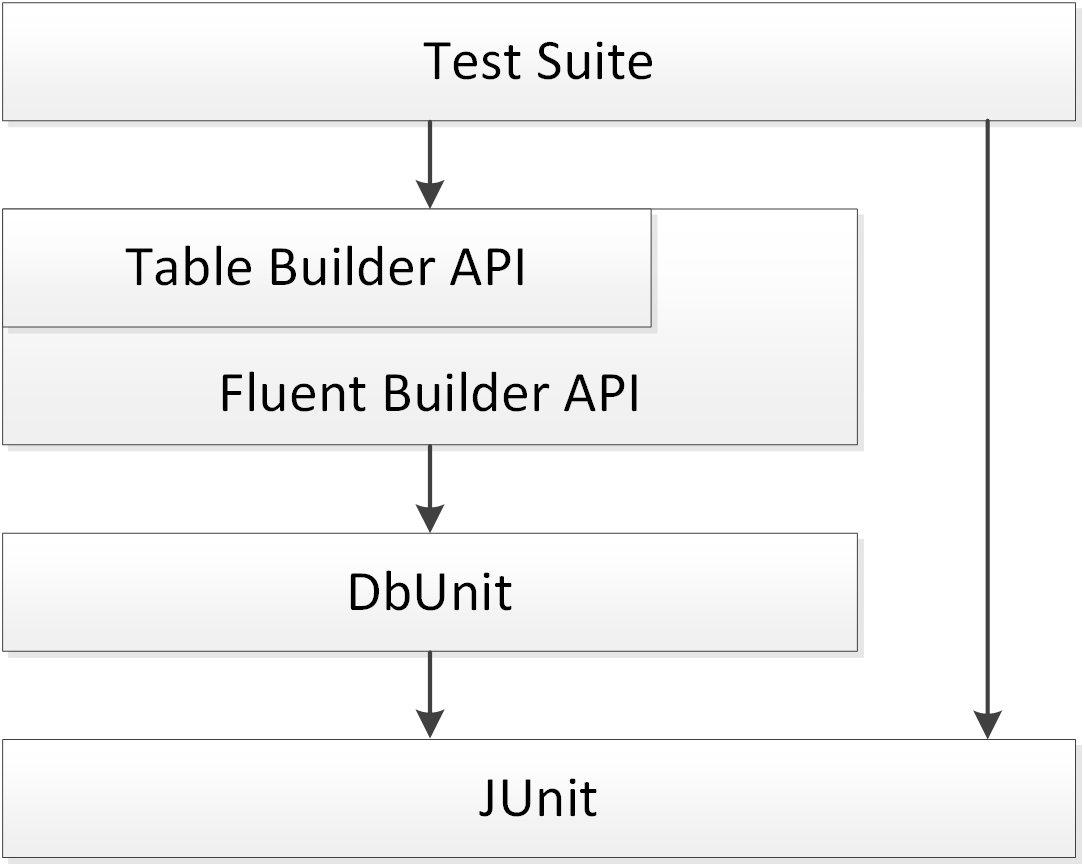
\includegraphics[scale=0.75]{images/realisierung/architektur.png}
	\caption{Architektur}\label{img:architektur}
\end{figure}
\todo{Neues Bild f�r Schichten}
	
Die neue Table Builder API stellt eine Schicht �ber der bisherigen Fluent Builder API dar. Neue Funktionen m�ssen 
jedoch nicht zwangsl�ufig in der Table Builder API hinzugef�gt werden, unter Umst�nden kann es vorteilhaft sein, sie
direkt in das Fluent Builder API zu integrieren. Gr�nde daf�r sind unter anderem:
\begin{itemize}
	\item \textbf{Code-Qualit�t}: Es gibt verschiedene Ans�tze, Klassen um neue Funktionen zu erweitern oder
	  ihr Verhalten zu �ndern. Unabh�ngig davon, ob auf Vererbung oder Delegation gesetzt wird, werden neue
		Datentypen ben�tigt.
			
	  Soll die Schicht der Fluent Builder API nicht ver�ndert werden, stellt Vererbung keine Option zur Erweiterungen
		von den Klassen dar, die von der Fluent-Builder-API-Schicht selbst instantiiert werden. Eine L�sung k�nnten
		Adapter-Klassen sein, die s�mtliche Methoden der zu adaptierenden Klasse beinhalten, aber auch die Erweiterungen.
		Eine solche Adapter-Klasse kann aus einer Vielzahl an Methoden bestehen, die nichts anderes machen, als die Aufgabe
		weiter zu delegieren.
			
		Insgesamt stellen Adapterklassen in Kombination mit Delegation keine elegante L�sungen dar. Die un�bersichtlicheren 
		und aufgebl�hten Klassenhierarchie ist dabei noch das kleinere Problem. Gravierender ist, dass innerhalb der
		Table Builder API konsequenterweise nur noch die Adapter-Klasse statt der urspr�nglichen Klasse als R�ckgabetyp
		von Methoden in Frage kommen darf. Das w�rde bedeuten, dass weitere Klassen adaptiert werden m�ssten, nur um den
		R�ckgabetyp anzupassen.
			
		Vererbung hat �hnliche Nachteile was die Klassenhierarchie betrifft und w�rde au�erdem noch �nderungen in der
		Fluent-Builder-API-Schicht nach sich ziehen. Wenn allerdings �nderungen innerhalb dieser Schicht gemacht werden,
		dann k�nnen die Erweiterungen auch direkt in dieser Schicht, also den bisherigen Klassen gemacht werden.
		So lange nur neue Funktionen hinzukommen und das Verhalten bestehender Methoden nicht ver�ndert wird, m�ssen bestehende
		Tests nicht an die neuen Schnittstellen angepasst werden.
			
	\item \textbf{Mehrwert gegen�ber SB Testing DB}: Auch wenn auf das neue Table Builder API verzichtet wird,
	  bietet das Fluent Builder API einen Mehrwert gegen�ber der bisherigen SB-Testing-DB-Implementierung.
	
  \item \textbf{Einheitliches Verhalten}: Beide APIs zeigen auf diese Weise ein einheitlicheres Verhalten.

\end{itemize}



\section{Entwurf der DSL}

... Vor- und Nachteile einzelner Entw�rfe ...

	\subsection{DSL-Entw�rfe}

		\subsubsection{Entwurf 1}
		
		Eine DSL, die sich stark an \textit{SB Testing DB} orientiert, k�nnte wie folgt aussehen:
		
		\begin{lstlisting}[caption=M�gliche DSL (1), label=listing:dslentwurf1]
HAASE = professor {
	name			"Haase"
	vorname   "Oliver"
	titel     "Prof. Dr."
  fakultaet "Informatik"
}

WAESCH = professor {
	name			"W�sch"
	vorname   "J�rgen"
	titel     "Prof. Dr.-Ing."
  fakultaet "Informatik"
}
	
VSYS = lehrveranstaltung {
	name			"Verteilte Systeme"
  sws       4
	ects      5
}
	
DPATTERNS = lehrveranstaltung {
	name 			"Design Patterns"
	sws       4
	ects      3
}

...

HAASE leitet VSYS
HAASE leitet DPATTERNS
HAASE beaufsichtigt	P_DPATTERNS
WAESCH beaufsichtigt P_VSYS
...

		\end{lstlisting}
		
		Diese DSL kommt ohne manuell vergebene ID-Nummern aus und verwendet Variablennamen f�r die Modellierung von Beziehungen. 
		Da f�r jeden Wert eine eigene Zeile verwendet wird, werden umfangreiche Daten schnell un�bersichtlich. Die Beschreibung
		der Beziehungen abseits der Definition der Daten erschwert den Umgang mit den Daten und die �bersicht ebenfalls.


		\subsubsection{Entwurf 2}
		
		Ein leicht abgewandelter Entwurf zeigt, wie sich die Beziehungen n�her an den eigentlichen Daten beschreiben lassen k�nnten.
		An dem Problem, dass die Daten relativ schnell in vertikaler Richtung wachsen, �ndert das jedoch nichts.
		

		\begin{lstlisting}[caption=M�gliche DSL (2), label=listing:dslentwurf2]
HAASE = professor {
	name      "Haase"
	vorname   "Oliver"
	titel     "Prof. Dr."
  fakultaet "Informatik"
	leitet    VSYS, DPATTERNS
	beaufsichtigt	P_DPATTERNS
}

WAESCH = professor {
	name      "W�sch"
	vorname   "J�rgen"
	titel     "Prof. Dr.-Ing."
  fakultaet "Informatik"
	beaufsichtigt	P_VSYS
}
	
VSYS = lehrveranstaltung {
	name			"Verteilte Systeme"
  sws       4
	ects      5
}
	
DPATTERNS = lehrveranstaltung {
	name 			"Design Patterns"
  sws       4
	ects      3
}

...
	\end{lstlisting}
	

		\subsubsection{Entwurf 3}
		
		Der dritte Entwurf versucht die Daten durch eine tabellarische Struktur �bersichtlich zu gestalten. Sie kommt mit
		wenig syntaktischem Ballast aus. Ein Label vor einer Tabelle dr�ckt aus, welche Daten folgen (Zeilen 1 und 6). Die
		Tabelle selbst beginnt mit einer Kopfzeile, die die Spaltenreihenfolge beschreibt (Zeilen 2 und 7). Einzelne Spalten
		werden vom Oder-Operator (|) getrennt. Die erste Spalte nimmt Zeilen-Identifikatoren auf und ist von den Daten
		mit Hilfe des Double-Pipe-Operators (||) abgrenzt.

		\lstSetTiny
		\begin{lstlisting}[caption=M�gliche DSL (3), label=listing:dslentwurf3]
professor:
REF    || name    | vorname  | titel            | fakultaet    | leitet          | beaufsichtigt
HAASE  || "Haase" | "Oliver" | "Prof. Dr."      | "Informatik" | VSYS, DPATTERNS | P_DPATTERNS   
WAESCH || "W�sch" | "J�rgen" | "Prof. Dr.-Ing." | "Informatik" |                 | P_VSYS
	
lehrveranstaltung:
REF       || name                | sws | ects
VSYS      || "Verteilte Systeme" | 4   | 5
DPATTERNS || "Design Patterns"   | 4   | 3

...
	\end{lstlisting}
	\lstSetNotmal
	
	Der Entwurf sieht vor, dass Beziehungen innerhalb beider Entit�tstypen ausgedr�ckt werden k�nnen. So kann
	eine Tabelle um Spalten f�r Beziehungen erg�nzt werden, die in dieser Form nicht Teil des relationalen
	Modells (\refimg{img:example_relational}) sind. Dazu geh�ren die Spalten "`leitet"' und "`beaufsichtigt"'
	der Professor-Tabelle. Erstere dr�ckt die 1:n-Beziehung zu einer Lehrveranstaltung aus, letztere die
	m:n-Beziehung zu Pr�fungen.
	
	Probleme bzw. Nachteile in der Darstellung k�nnen auftreten, wenn die L�nge der Werte in einer Spalte stark
	variiert. Die Spaltenbreite wird vom l�ngsten Element bestimmt. Der Entwickler ist selbst daf�r verantwortlich,
	die �bersichtliche Darstellung einzuhalten. Auf Tabulatoren sollte unter  Umst�nden verzichtet werden, da sie von
	verschiedenen Editoren unterschiedlich dargestellt werden k�nnen. Bei vielen Spalten w�chst diese Darstellung
	horizontal. Bei optionalen Spalten bzw. kaum genutzte Spalten kann die tabellarische Darstellung un�bersichtlich
	werden.
	
	Einige Entwicklungsumgebungen wie Eclipse bieten spezielle Block-Bearbeitungsfunktionen an, die beim Arbeiten an
	einer Tabellen-DSL hilfreich sein kann. So k�nnen beispielsweise in einer Spalte �ber mehrere Zeilen hinweg 
	Leerzeichen eingef�gt oder entfernt werden.
	
	Zur besseren �bersicht kann es bei gr��eren Tabellen sinnvoll sein, den Tabellenkopf zu wiederholen.
	
  \subsection{Entscheidung}

	Der dritte Entwurf zeigt, dass eine tabellarische Schreibweise viele Schw�chen der anderen Varianten ausmerzt.
	Die Darstellung wirkt �bersichtlich, da Tabellen ... \todo{Hier w�re eine Quelle super, dass Menschen vertraut
	mit Tabellen sind}

\todo{Einfache Sprachdefinition, Grammatik}
	

\section{Implementierungsvorbereitung}
\label{sec:modellierung:wahlimplementierung}

Da sich die DSL in die bisherige Werkzeug-Kette von Seitenbau integrieren lassen soll
(\refsec{sec:anforderungen:allgemeineanforderungen}), sollte die DSL in Java nutzbar sein. Zwar kann eine DSL
grunds�tzlich auch in Java realisiert werden, doch die M�glichkeiten diesbez�glich sind relativ eingeschr�nkt 
und die DSL sieht immer noch nach Java aus. Es lassen sich allerdings auch andere Sprachen im Java-Umfeld nutzen.

Eine davon ist \textit{Groovy}. Groovy ist eine dynamisch typisierte Sprache\footnote{Im Gegensatz zu statisch 
typisierten Sprachen finden bei dynamisch typisierten Typ-�berpr�fungen �berwiegend zur Laufzeit statt.}, die
direkt in Java-Bytecode �bersetzt wird und damit auch in einer Java Virtual Machine ausgef�hrt wird. Sie teilt
sich das Objekt-Modell mit Java, so dass aus Groovy heraus instantiierte Objekte auch in der Host-Anwendung 
nutzbar sind (und umgekehrt). Auch wenn Java-Code bis auf wenige Ausnahmen g�ltiger Groovy-Code und sich dort
gleich verh�lt, enth�lt Groovy Techniken, die den Code mehr wie eine nat�rliche Sprache aussehen lassen.
So kann oftmals auf die Semikolons am Ende einer Anweisung verzichtet werden, und auch auf das Einklammern
von Parametern kann bei Methoden aufrufen verzichtet werden (wenn die Methode genau einen Parameter erwartet).
Au�erdem kann statt dem Punkt zwischen Objekt und Methode beim Aufruf verzichtet werden.

Listing \ref{listing:groovyexamples} zeigt einen Befehl einmal in typischer Java-Syntax und einmal mit den
Syntax-Vereinfachungen von Groovy:

	\begin{lstlisting}[caption=Vereinfachung von Ausdr�cken in Groovy, label=listing:groovyexamples]
myList.append("value 1").append("value 2");
myList append "value 1"  append "value 2"  
	\end{lstlisting}

Groovy hebt sich ferner durch die M�glichkeit Operatoren zu �berladen und durch Closures (Funktionsabschl�sse) von
Java ab. Ein Closure ist ein Codeblock, der wie eine Funktion aufgerufen und genutzt werden kann. In Java lassen
sich Closures mit syntaktisch umfangreicheren Methoden-Objekten nachbilden. Ein Methoden-Objekt stellt eine
Instanz einer (m�glicherweise anonymen) Klasse dar, die nur eine Methode implementiert. \cite[40]{GROOVY_IM_EINSATZ} 
\todo{Quelle Kent Beck Smalltalk Best Practice Patterns} 
Die Unterst�tzung zur Meta-Programmierung stellt sich beim Implementieren einer DSL ebenfalls als n�tzlich
heraus. Dadurch ist es z.B. m�glich, abgeschlossene Klassen innerhalb von Groovy um Methoden zu erweitern oder auf
den Zugriff von nicht definierten Klassenelementen zu reagieren.

Aus diesen Gr�nden empfiehlt Ghosh in \cite[148]{DSLS_IN_ACTION} Groovy als Host f�r DSLs in Verbindung
mit Java-Anwendungen. 

	\subsection{Implementierungsvarianten}
	\label{sec:modellierung:implementierung:varianten}
	
	Eine DSL kann auf unterschiedliche Arten implementiert werden. Groovy bietet daf�r zwei M�glichkeiten der
	Meta-Programmierung an: Laufzeit-Meta-Programmierung und Compiler-Zeit-Meta-Programmierung, letzteres in Form von
	AST-Transformationen. Beide Ans�tze bieten individuelle Vorteile, die im folgenden diskutiert werden.  
	\nomenclature{AST}{Abstract Syntax Tree}


		\subsubsection{Laufzeit-Meta-Programmierung}
	  \label{sec:modellierung:implementierung:varianten:laufzeit}
		
		Eine M�glichkeit, die DSL mit Hilfe von Laufzeit-Meta-Programmierung zu implementieren sieht eine 
		Klasse zum Parsen von Closures vor, die eine Tabelle beinhalten. Diese Klasse, \textit{TableParser},
		enth�lt daf�r die Methode \texttt{parseTableClosure}. Die Methode soll als Ergebnis eine Liste
		von Tabellenzeilen zur�ckliefern. Da an dieser Stelle noch keinerlei Interpretation der Tabellenwerte
		durchgef�hrt wird, stellt eine Tabellenzeile selbst ebenfalls eine Liste dar - aus den Objekten
		der Spalten.
		
		Der Ansatz ist, Operator-�berladen f�r das Parsen zu verwenden. Soll ein bin�rer Operator\footnote{Bin�r
		bezogen auf die Verkn�pfung zweier Werte und nicht auf das Zahlensystem} implementiert werden, ist die
		�bliche Vorgehensweise in Groovy, die Klasse des linken Operanden um eine entsprechende Methode f�r den
		Operator zu erweitern. Diese Methode tr�gt einen vorgegebenen Namen und erwartet als bin�rer Operator 
		den rechten Operanden als Parameter (eine  �bersicht findet sich beispielsweise in 
		\cite[58]{GROOVY_IM_EINSATZ}).
		
		Auch wenn sich dank der M�glichkeiten der Meta-Programmierung Klassen in Groovy zur Laufzeit um Methoden
		erg�nzen lassen, ist dieses Vorgehen nicht empfehlenswert um eine Tabelle zu parsen. Dieser wenig
		generische Ansatz m�sste jeden in den Tabellen m�gliche Datentyp ber�cksichtigen - kommen neue Datentypen
		hinzu, m�sste der Code erweitert werden.
		\todo{M�gliche ungewollte Seiteneffekte}
		
		Groovy bietet allerdings auch eine zweite M�glichkeit f�r das Operator-�berladen an. Anstatt den Operator
		als Methode dem linken Operand (bzw. der Klasse) hinzuzuf�gen, wird er als statische Methode (in einer
		beliebigen Klasse) realisiert. Da eine statische Methode ohne Kontext ausgef�hrt wird, ben�tigt sie alle
		beteiligten Operanden als Parameter. Eine solche Methode wird als Kategoriemethode bezeichnet. 
		�ber das Schl�sselwort \textit{use}\footnote{\textit{use} wird in der Literatur meistens als Schl�sselwort
		bezeichnet, tats�chlich handelt es sich jedoch um eine Groovy-Methode in \texttt{java.lang.Object}}
		k�nnen die Kategoriemethoden in einem Closure verwendet werden. \cite[192]{GROOVY_IM_EINSATZ} 
		
		Listing \ref{listing:opoverloading.tableparser.base} zeigt das Grundger�st des Tabellenparsers:
		
		\begin{lstlisting}[caption=Tabellen-Parser Grundger�st mit Operator-�berladen, label=listing:opoverloading.tableparser.base]
class TableParser {
  
  static or(self, arg) {
		// ...
  }

  def parseTableClosure(Closure tableData){
    use(TableParser) {
      tableData()
    }
  }

}
		\end{lstlisting}
		
		Die Methode \texttt{or} erwartet zwei Parameter vom Typ \textit{Object}. Obwohl in Groovy alle Typen von
		\textit{Object} abgeleitet sind, gibt es Oder-Ausdr�cke, bei denen diese Methode nicht aufgerufen wird.
		Ein in der Klasse definierter Operator mit passenden Datentypen wird dieser allgemeinen Methode bevorzugt,
		z.B. bei zwei \textit{Integer}-Werten. Doch auch solche Operationen lassen sich �berschreiben, wenn f�r
		die Datentypen passende Kategoriemethoden definiert werden.

		Der Parser in der Form kann noch nicht mit selbst definierten Variablennamen f�r die Abbildung von Referenzen
		umgehen. Aus diesem Grund wird eine Methode \texttt{getProperty} definiert, die f�r jeden Variablennamen
		in der Tabelle aufgerufen werden soll. Dazu muss der Ausf�hrungskontext des Closures auf die Instanz
		des Tabellenparsers ge�ndert werden. Die �nderungen sind in Listing \ref{listing:opoverloading.tableparser.extended}
		dargestellt.

		\begin{lstlisting}[caption=Tabellen-Parser Grundger�st mit Operator-�berladen, label=listing:opoverloading.tableparser.extended]
class TableParser {
  
  static or(self, arg) {
		// ...
  }
	
  static or(Integer self, Integer arg) {
		// ...
  }

  static or(Boolean self, Boolean arg) {
		// ...
	}
	
	def getProperty(String property) {
		// ...
  }
	

  def parseTableClosure(Closure tableData){
    use(TableParser) {
      tableData.delegate = this		// Change closure's context
      tableData.resolveStrategy = Closure.DELEGATE_FIRST
      tableData()
    }
  }

}
		\end{lstlisting}
		
		Die statischen Methoden haben keinen Zugriff auf Instanz-Variablen der Klasse \textit{TableParser}. Ihre Ergebnisse
		k�nnen sie demnach auch nur in statische Elementen aufbewahren. Um die Klasse Thread-sicher zu machen, d.h. das
		gleichzeitige Parsen von Tabellen aus verschiedenen Threads heraus, wird f�r die Ergebnisse eine threadlokale
		Liste verwendet. \todo{thread local erkl�ren mit quelle} \cite{JAVA_CONCURRENCY_IN_PRACTICE}

				
		Die Laufzeit-Meta-Programmierung kann die Syntax der Sprache nicht beliebig erweitern. Groovy kennt keinen
		Double-Pipe-Operator. Deshalb kann dieser weder �berladen noch �ber Laufzeit-Meta-Programmierung eingef�hrt
		werden. Folglich ist es nicht m�glich, den dritten Entwurf �ber reine Laufzeit-Meta-Programmierung zu
		realisieren. Allerdings kann eine Syntax erreicht werden, die dem Entwurf sehr nahe kommt
		(\reflst{listing:dslentwurf3laufzeit}). Ein Platzhalter (Unterstrich) verhindert Syntax-Fehler, wenn in
		einer Spalte kein Wert vorkommt (siehe Zeile 4, Spalte "`leitet"'). Der Platzhalter k�nnte auch verwendet
		werden, um einem Datensatz keinen Bezeichner f�r Referenzen zu zu weisen. Aus Sicht des Parsers stellt
		der Unterstrich eine Variable dar.
		
		\lstSetTiny
		\begin{lstlisting}[caption=DSL-Entwurf 3 f�r Laufzeit-Meta-Programmierung angepasst, label=listing:dslentwurf3laufzeit]
def fixture = [
  professor: {
	  REF    | name    | vorname  | titel            | fakultaet    | leitet           | beaufsichtigt
		WAESCH | "W�sch" | "J�rgen" | "Prof. Dr.-Ing." | "Informatik" | _                | P_VSYS
		HAASE  | "Haase" | "Oliver" | "Prof. Dr."      | "Informatik" | VSYS & DPATTERNS | P_DPATTERNS
  },

  lehrveranstaltung: {
    REF       | name                | sws | ects
    VSYS      | "Verteilte Systeme" | 4   | 5    
    DPATTERNS | "Design Patterns"   | 4   | 3    
  },
		
  ...
]		
		\end{lstlisting}
		\lstSetNotmal
		
		

		\subsubsection{AST-Transformation}
		
		Die AST-Transformationen stellen ein m�chtiges Werkzeug zur Erweiterung der Syntax der Sprache dar. Mit Hilfe
		der Transformationen ist es m�glich, �nderungen am AST durchzuf�hren, bevor er in Java-Bytecode �bersetzt wird.
		
		Dass AST-Transformationen mehr syntaktische M�glichkeiten bieten, zeigt sich auch daran, dass hier der 
		Double-Pipe-Operator verwendet werden kann. Au�erdem k�nnen Labels erkannt werden und Daten einer Tabelle
		m�ssen nicht zwangsl�ufig in einem eigenen Block definiert werden.
		
		Allerdings muss zum Auswerten einer Tabelle bei AST-Transformationen ein relativ gro�er Aufwand betrieben werden.
		Der Zugriff auf den AST erfolgt dabei �ber das Visitor-Pattern
		(\cite[331ff]{DESIGN_PATTERNS}).
		
	\subsection{Implementierungsentscheidung}
	\label{sec:implementierung:entscheidung}
	
	Der Vergleich zwischen Laufzeit-Meta-Programmierung und AST-Transformation zeigt, dass sich Groovy als Host-Sprache
	f�r die DSL eignet. Die Laufzeit-Meta-Programmierung erlaubt zwar weniger Anpassungen an die Sprache, ist aber f�r
	die gew�nschte DSL ausreichend und die Umsetzung einfacher. 
		

\section{�nderungen am Generator-Modell}
\label{sec:modellierung:generatormodell}


  \subsection{Builder-Klassen f�r das Datenbankmodell}
	\label{sec:modellierung:generatormodell:builder}
	
	Bei den Builder-Klassen f�r die Modellierung des zu Grunde liegenden Datenbankmodells wird auf Abw�rtskompatiblit�t verzichtet.
	W�hrend das alte API auf �berladene Methoden mit vielen Parametern setzt, ist das neue API entsprechend dem Builder-Pattern
	umgesetzt (Quelle). So enth�lt das alte API neun Methoden zum Hinzuf�gen einer Spalte in einer Tabelle enth�lt, wovon eine
	als \textit{deprecated} eingestuft ist. Dieses Design ist un�bersichtlich und nur schwer erweiterbar. Jeder weitere optionale
	Parameter k�nnte die Anzahl der Methoden verdoppeln. Demgegen�ber gibt es beim Builder-Pattern f�r jeden optionalen Parameter
	eine einzelne Set-Methode.
	
	Die neuen Builder-Klassen decken den Funktionsumfang der alten API ab. So werden Flags f�r Spalten nicht mehr �ber 
	ein \texttt{EnumSet} festgelegt, sondern �ber Methoden f�r die vordefinierten Flags. In Abschnitt 
	\ref{sec:modellierung:generatormodell:flags}  wird weiter auf das Thema Flag eingegangen. Dar�ber hinaus bieten die
	neuen Klassen die M�glichkeit, Beschreibungen zu Tabellen und Spalten hinzu zu f�gen. Diese werden bei der Code-Generierung
	f�r die Erstellung von JavaDoc-Kommentaren verwendet (\refsec{sec:modellierung:realisierung:javadoc}).
	
	\todo{Abh�ngigkeitsdiagramm der neuen Builder-Klassen?}
	
	\subsection{Spalten-Flags}
	\label{sec:modellierung:generatormodell:flags}
	
	SB Testing DB sieht verschiedene Flags f�r Spalten vor, die in einem \textit{Enum} zusammengefasst sind. Alle f�r eine Spalte 
	gesetzten Flags m�ssen beim Hinzuf�gen einer Spalte �ber ein \textit{EnumSet} �bergeben werden. Bei dem neuen Builder-API werden
	die Flags �ber spezielle Methoden gesetzt.
	
	Zu den in STU enthaltenen Standard-Spalten-Flags geh�ren:
	\begin{itemize}
		\item \textbf{Identifkator-Spalte}: Als Identifikator-Spalte wird die Spalte bezeichnet, die einen f�r die Zeile einmaligen
		  Wert enth�lt, �ber die eine Zeile zweifelsfrei identifiziert werden kann. In dieser Eigenschaft �hnelt sie dem Prim�rschl�ssel
			in Datenbanken. Es bietet sich an, Prim�rschl�ssel als Identifikator-Spalte zu modellieren. Dennoch gibt es keine Kausalit�t
			zwischen Identifikator-Spalte und Prim�rschl�ssel: Ein Prim�rschl�ssel muss nicht als Identifikator-Spalte modelliert werden,
			und eine Identifikator-Spalte muss kein Prim�rschl�ssel sein.
			
			Die Identifikator-Spalte ist die Spalte, die bei Beziehungen verwendet wird, wenn das Ziel eine Tabelle und nicht eine Spalte
			der Tabelle ist. Das Flag wird �ber die Methode \texttt{identifierColumn} aktiviert. Dabei werden die Flags Unver�nderbar und
			Einmalig ebenfalls aktiviert.

		\item \textbf{Next-Value-Methode}: SB Testing DB (und damit auch STU) bietet die M�glichkeit, Werte-Generatoren zu verwenden
		  um einen Spaltenwert manuell oder auch automatisch mit einem generierten Wert zu belegen. Aufgerufen wird der Generator �ber
			eine sogenannte Next-Value-Methode auf dem RowBuilder. Ihr Name setzt sich aus dem Pr�fix \texttt{next} und dem Spaltennamen
			zusammen. Der Generator erzeugt f�r die jeweilige Spalte allerdings nur dann eine Next-Value-Methode, wenn das entsprechende
			Flag �ber \texttt{addNextMethod()} aus dem Builder-API gesetzt wurde. Standardm��ig muss die Next-Value-Methode manuell
			aufgerufen werden, �ber ein Flag kann dies auch automatisch erfolgen.
			
		\item \textbf{Automatischer Aufruf der Next-Value-Methode}: Ist dieses Flag aktiviert, wird die Next-Value-Methode beim 
		  Anlegen einer neuen Tabellenzeile automatisch aufgerufen. Beim Setzen des Flags �ber die Builder-Methode
			\texttt{autoInvokeNext()} wird automatisch auch das Flag zum Generieren der Next-Value-Methode gesetzt. 
			
		\item \textbf{Auto Increment}: ... DBUNIT-Flag ... implizit addNextMethod
		
		\item \textbf{Unver�nderbar}: Ist dieses Flag gesetzt, kann ein Wert in einer Spalte nur ein Mal gesetzt werden, und danach
		  nicht mehr ver�ndert werden. Wenn das Flag zum automatischen Aufruf der Next-Value-Methode aktiviert ist, kann der
			automatisch erzeugte Wert allerdings �berschrieben werden. Die Methode zum
			Aktivieren des Flags hei�t \texttt{immutable()}.
		
		\item \textbf{Einmalig}: Dieses Flag gibt an, dass die Werte einer Spalte nur jeweils ein Mal vorkommen, und sie deshalb
		  zur Identifikation einer Zeile verwendet werden k�nnen. Das Flag sollte auch nur dann verwendet werden, wenn eine solche
			Identifikation erw�nscht ist.
			
			Aufgrund des Anwendungszwecks wird das Flag Unver�nderbar implizit aktiviert. Das Einmalig-Flag wird �ber die Methode
			\texttt{unique()} aktiviert und setzt keine Unique-Eigenschaft in der Datenbank voraus.
		  
	\end{itemize}
	
	
	\subsection{Modellierung von Relationen �ber Builder-Klassen}
	
	
	\subsection{Alte und neue Builder-Klassen im Vergleich}
	\label{sec:modellierung:generatormodell:buildervergleich}
	
	\begin{lstlisting}[caption=Beispiel SB-Testing-DB-Builder, label=listing:model:builder:old]
database("Hochschule");
packageName("com.seitenbau.sbtesting.dbunit.hochschule");

Table professoren = addTable("professor")
		.addColumn("id", DataType.BIGINT, Flags.AutoInvokeNextIdMethod) 
		.addColumn("name", DataType.VARCHAR)
		.addColumn("vorname", DataType.VARCHAR)
		.addColumn("titel", DataType.VARCHAR)
		.addColumn("fakultaet", DataType.VARCHAR);

Table lehrveranstaltungen = addTable("lehrveranstaltung")
		.addColumn("id", DataType.BIGINT, Flags.AutoInvokeNextIdMethod)
		.addColumn("professor_id", DataType.BIGINT, professoren.ref("id"))
		.addColumn("name", DataType.VARCHAR)
		.addColumn("sws", DataType.INTEGER)
		.addColumn("ects", DataType.DOUBLE);
  \end{lstlisting}
	
	\begin{lstlisting}[caption=Beispiel STU-Builder, label=listing:model:builder:new]
database("Hochschule");
packageName("com.seitenbau.stu.dbunit.hochschule");
enableTableModelClassesGeneration();

Table professoren = table("professor")
		.description("Die Tabelle mit den Professoren der Hochschule")
		.column("id", DataType.BIGINT) 
			.identifierColumn() 
			.autoInvokeNext()
		.column("name", DataType.VARCHAR)
		.column("vorname", DataType.VARCHAR)
		.column("titel", DataType.VARCHAR)
		.column("fakultaet", DataType.VARCHAR)
	.build();

Table lehrveranstaltungen = table("lehrveranstaltung")
		.description("Die Tabelle mit den Lehrveranstaltungen der Hochschule")
		.column("id", DataType.BIGINT)
			.identifierColumn() 
			.autoInvokeNext()
		.column("professor_id", DataType.BIGINT)
			.references(professoren)
				.local("geleitetVon")
					.description("Gibt an, von welchem Professor eine Lehrveranstaltung geleitet wird.")
				.remote("leitet")
					.description("Gibt an, welche Lehrveranstaltungen ein Professor leitet.")
		.column("name", DataType.VARCHAR)
		.column("sws", DataType.INTEGER)
		.column("ects", DataType.DOUBLE)
	.build();	
	\end{lstlisting}



\section{Realisisierung}
\label{sec:modellierung:realisierung}

% Fluent Builder API Java basiert
% Table DSL Groovy basiert





- http://martinfowler.com/eaaCatalog/gateway.html\\
- http://martinfowler.com/eaaCatalog/repository.html\\
- http://martinfowler.com/eaaCatalog/registry.html
	
	
	
	

	
	\subsection{Allgemeiner Tabellenparser}
	\label{sec:modellierung:realisierung:parser}
	
	Der Tabellenparser basiert auf dem in Abschnitt \ref{sec:modellierung:implementierung:varianten:laufzeit} gezeigten
	Quellcode. 
	- TableParser (Groovy)
	- TableParserContext
	- TableParserCallback
	- zeilenweise wegen Exceptions
	- Groovy-Anteil minimiert
	- Diagramm :-)
	
	
	\subsection{Builder f�r DataSet}
	\label{sec:modellierung:realisierung:builderdataset}
	
	\subsection{Builder f�r Tabellen}
	\label{sec:modellierung:realisierung:buildertabellen}
	
	\subsection{ColumnBinding}
	\label{sec:modellierung:realisierung:columnbinding}
	
	ColumnBindings sind Variablen in den jeweiligen Tabellen-Adaptern, ihre Namen entsprechenden den Tabellenspalten.
	Sie l�sen zwei Probleme:
	
	\begin{enumerate}
		\item \textbf{Tool-Support}: Elemente der Tabellen-Header-Zeile, Auto-Vervollst�ndigung, Liste von nutzbaren Elementen
		
		\item \textbf{Operationen f�r den Parser}: Operationen auf den ColumnBindings vereinfachen den Tabellen-Parser. Der
		  Tabellen-Parser setzt die Werte auf den RowBuildern. Die Setter-Namen h�ngen aber vom Namen der Spalte ab. Anstelle
			eines generischen Ansatzes �ber Reflection, wird ein allgemeiner Setter auf der ColumnnBinding-Klasse verwendet,
			und in den jeweiligen zu den Spalten zugeh�rigen ColumnBindings wird auf den eigentlichen Setter auf dem RowBuilder
			delegiert.
			
			Au�erdem kann der Parser auch Informationen zu der Spalte abfragen, z.B. ob es sich um ein Feld mit einmaligen Werten
			handelt, die zur Identifizierung genutzt werden k�nnen. F�r solche Spalten gibt es auch eine Such-Methode auf dem
			ColumnBinding, die den zugeh�rigen RowBuilder zur�ckliefern, falls es einen gibt.
	\end{enumerate}
	
	\subsection{Referenzen und Scopes}
	\label{sec:modellierung:realisierung:refs_and_scopes}
	
	Neben der M�glichkeit, Daten tabellarisch zu modellieren, geh�ren die neuen Referenz-Datentypen zu der wichtigsten Erweiterung.
	In STU ist eine Referenz eine Art Stellvertreter f�r eine Entit�t (Tabellenzeile). Die Referenz kann bei der Modellierung 
	anstelle konkreter Werte (wie Prim�rschl�ssel) verwendet werden, oder bei Such-Anfragen anstelle von konkreten Werten
	(mehr dazu in Abschnitt \ref{sec:modellierung:realisierung:apierweiterungen}). 
	
	Referenzen m�ssen an ihre Datens�tze gebunden werden. Im Table Builder API ist daf�r die Spalte \textit{REF} vorgesehen,
	die in jeder Tabelle genutzt werden kann, das Fluent Builder API bietet auf den RowBuilder-Klassen die Methode \texttt{bind()}.
	Listings \ref{listing:ref:bindingtable} und \ref{listing:ref:bindingfluent} zeigen die Modellierung der selben Zeile einmal 
	mit dem neuen Table Builder API und einmal mit dem erweiterteren Fluent Builder API.
	
	\begin{lstlisting}[caption=Binden von Referenzen (Table Builder API), label=listing:ref:bindingtable]
professorTable.rows {
  REF    | name    | vorname  | titel            | fakultaet
  WAESCH | "W�sch" | "J�rgen" | "Prof. Dr.-Ing." | "Informatik"
	...
}
	\end{lstlisting}
  
	\begin{lstlisting}[caption=Binden von Referenzen (Fluent Builder API), label=listing:ref:bindingfluent]
table_Professor.insertRow()
  .bind(WAESCH)
	.setName("W�sch")
	.setVorname("J�rgen")
	.setTitle("Prof. Dr.-Ing.")
	.setFakultaet("Informatik")
...
	\end{lstlisting}
	
	Da Referenzen die zugeh�rigen RowBuilder kennen, k�nnen ihre Werte auch direkt auf der Referenz abgefragt werden 
	(\reflst{listing:ref:valueaccess}).
	
	\begin{lstlisting}[caption=Zugriff auf Werte �ber Referenzen, label=listing:ref:valueaccess]
WAESCH.getName()    // Java style
WAESCH.name         // Groovy style
	\end{lstlisting}
	
	Dar�ber hinaus k�nnen �ber Referenzen Beziehungen modelliert werden. Sie enthalten Methoden zum Ausdr�cken von Beziehungen.
	Die Methodennamen entsprechen den im Generator-Modell angegebenen Relationsnamen. Listing \ref{listing:ref:relations} zeigt
	ein Beispiel,wie die Relation zwischen einem Professor und einer Pr�fung modellieren l�sst.
	\begin{lstlisting}[caption=Zugriff auf Werte �ber Referenzen, label=listing:ref:relations]
WAESCH.beaufsichtigt(P_VSYS)
	\end{lstlisting}
	
	Die Referenzen m�ssen vor ihrer Nutzung definiert (also deklariert und instantiiert) werden. Zwar k�nnten in Groovy auch nicht
	explizit definierte Referenzen verwendet werden (z.B. �ber die Methode \texttt{getPropery()}, allerdings w�rde Tool-Unterst�tzung
	verloren gehen (z.B. beim Umbenennen von Referenzen, Erkennen von Tippfehlern bei Bezeichnern). Au�erdem k�nnten sie auch nicht
	im normalen Java-Code verwendet werden. Es bietet sich an, sie als globale Variablen zu definieren. Verschiedene DataSets (mit
	dem selben Datenbank-Modell) k�nnen die selben Referenzen nutzen, auch wenn  sie unterschiedliche Werte repr�sentieren.
	
	Damit die selben Referenzen in unterschiedlichen DataSets genutzt werden k�nnen, werden die RowBuilder immer im Kontext des
	gerade aktiven DataSets gebunden. Das aktive DataSet wird �ber die \textit{DataSetRegistry} festgelegt (und abgefragt). Pro
	Datenbank-Modell ist immer ein (oder kein) DataSet aktiv. Das hei�t, dass wenn verschiedene Datenbank-Modelle genutzt werden,
	gleichzeitig ein DataSet aus dem ersten Modell, aber auch ein anderes DataSet aus einem anderen Modell aktiv sein kann.
	
	
	\subsection{Komposition von DataSets}
	\label{sec:modellierung:realisierung:kompositiondatasets}
	
	

  \subsection{Erweiterungen in generierter API}
	\label{sec:modellierung:realisierung:apierweiterungen}
	
	Die meisten Erweiterungen an der Fluant-Builder-API-Schicht betreffen die M�glichkeit, Ref-Typen statt konkreter Werte
	zu verwenden. Dazu geh�ren unter anderem:
	
	\begin{itemize}
		\item \textbf{RowBuilder}: Die Erweiterungen der RowBuilder betreffen vor allem die verbesserten M�glichkeiten
		  Relationen auszudr�cken. So gibt es f�r Spalten, die eine Relation zu einer anderen Spalte enthalten, nun neben
			einem Setter f�r den konkreten Wert (z.B. des Fremdschl�ssels) einen Setter zum Setzen des entsprechenden
			Ref-Typs. 
			
		  Anstelle des von der Ref repr�sentierten Wertes wird die Ref selbst im RowBuilder abgespeichert. Das hat zwei
			Vorteile:
     	\begin{enumerate}
		    \item \textbf{Reihenfolge}: Die Modellierung der Daten ist in diesem Fall keiner strengen Reihenfolge unterworfen.
				  Es ist egal, ob die Zeile, auf die Bezug genommen wird, �berhaupt schon initialisiert wurde.

		    \item \textbf{Konsistenz}: Die Werte werden nicht redundant gespeichert. Wird der Wert an einer Stelle ge�ndert,
				  ist dieser Wert unmittelbar im gesamten DataSet so sichtbar.
		  \end{enumerate}
			
		\item \textbf{Future Values}: Eine der wenigen Erweiterungen, die nicht auf die Einf�hrung der Ref-Typen zur�ckzuf�hren
		  sind, sind Future Values. Dabei handelt es sich um Werte, die erst beim Abfragen ausgewertet werden. Dies kann n�tzlich
			sein, wenn sich Werte abh�ngig von anderen Daten �ndern. Listing \ref{listing:futurevalues} zeigt ein Beispiel, in der
			die Lehrveranstaltungstabelle um eine Spalte erweitert wurde. Diese Spalte soll die Anzahl der Tutoren aufnehmen, die
			die Lehrveranstaltung betreuen.
		
	    \begin{lstlisting}[caption=Beispiel Lazy Valunes, label=listing:futurevalues]
class HochschuleDataSet extends HochschuleBuilder
{

  def tables() {
        
    lehrveranstaltungTable.rows {
      REF       | name                | sws | ects | tutoren
      VSYS      | "Verteilte Systeme" | 4   | 5    | tutors(VSYS)
      DPATTERNS | "Design Patterns"   | 4   | 3    | tutors(DPATTERNS)
    }
    
    ...
  }
    
  ...

  // returns a Closure which is threated as future value
  def tutors(LehrveranstaltungRef ref) {
    return {
      // findWhere throws an exception if no rows are found
      if (isttutorTable.getWhere.lehrveranstaltungId(ref).present) { 
        def rows = isttutorTable.findWhere.lehrveranstaltungId(ref);
        return rows.getRowCount()
      }
      return 0;
    }
  }
}
  	  \end{lstlisting}
			
			Durch die Nutzung von Future Values enth�lt die Tabelle immer die korrekte Anzahl, ohne dass beim Modellieren
	    der Tutoren-Beziehungen Anpassungen notwendig wurden. In Groovy k�nnen Closures verwendet werden, ...


    \item \textbf{findWhere}: Das bisherige API sah Suchen von Zeilen in einer Tabelle ausschlie�lich �ber konkrete Werte
		  vor. Die Erweiterung erm�glicht es, dass Ref-Typen statt konkreter Werte verwendet werden k�nnen. Werden beispielsweise 
			in der Professor-Tabelle alle Professoren mit einem bestimmten Vornamen gesucht und als Such-Wert eine 
			Professor-Referenz �bergeben, werden alle Professoren mit diesem Vornamen gesucht. Listing
			\ref{listing:apierweiterung:findexample} zeigt zwei Such-Anfragen, die beide auf den Beispieldaten das selbe Ergebnis
			liefern.
	
	    \begin{lstlisting}[caption=Such-Beispiele, label=listing:apierweiterung:findexample]
dataSet.table_Professor.findWhere.vorname("Oliver");
dataSet.table_Professor.findWhere.vorname(HAASE);
	    \end{lstlisting}

		  
	  \item \textbf{getWhere}:
		  - Zus�tzlich zu findWhere
	  
		\item \textbf{find}: Sind die einfachen Such-Anfragen �ber \texttt{findWhere} bzw. \texttt{getWhere} nicht m�chtig genug,
		  k�nnen mit Hilfe von \texttt{find} Filter-basierte Suchen durchgef�hrt werden. In Listing \ref{listing:find} wird
			ein Filter gezeigt, der alle Professoren findet, deren Vorname die L�nge sechs hat.
			
	    \begin{lstlisting}[caption=Beispiel f�r find, label=listing:find]
Filter<RowBuilder_Professor> FILTER = 
  new Filter<RowBuilder_Professor>() 
	  {
		  @Override
		  public boolean accept(RowBuilder_Professor value)
		  {
			  return value.getVorname().length() == 6;
		  }
	  };
		
RowCollection_Professor profs = dataSet.professorTable.find(FILTER);
  	  \end{lstlisting}
			
			In Groovy k�nnen auch direkt Closures �bergeben werden, die als Argument einen entsprechenden RowBuilder �bergeben
			bekommen.
	  
    \item \textbf{foreach}:
	    \begin{lstlisting}[caption=Beispiel f�r foreach, label=listing:foreach]
Action<RowBuilder_Professor> ACTION = 
  new Action<RowBuilder_Professor>() 
	  {
		  @Override
		  public void call(RowBuilder_Professor value)
		  {
			  System.out.println("Professor: " + value.getName());
		  }
	  };
	
dataSet.professorTable.foreach(ACTION);
  	  \end{lstlisting}
				
	\end{itemize}
	
	\subsection{JavaDoc}
	\label{sec:modellierung:realisierung:javadoc}

\begin{figure}[H]
	\centering
	 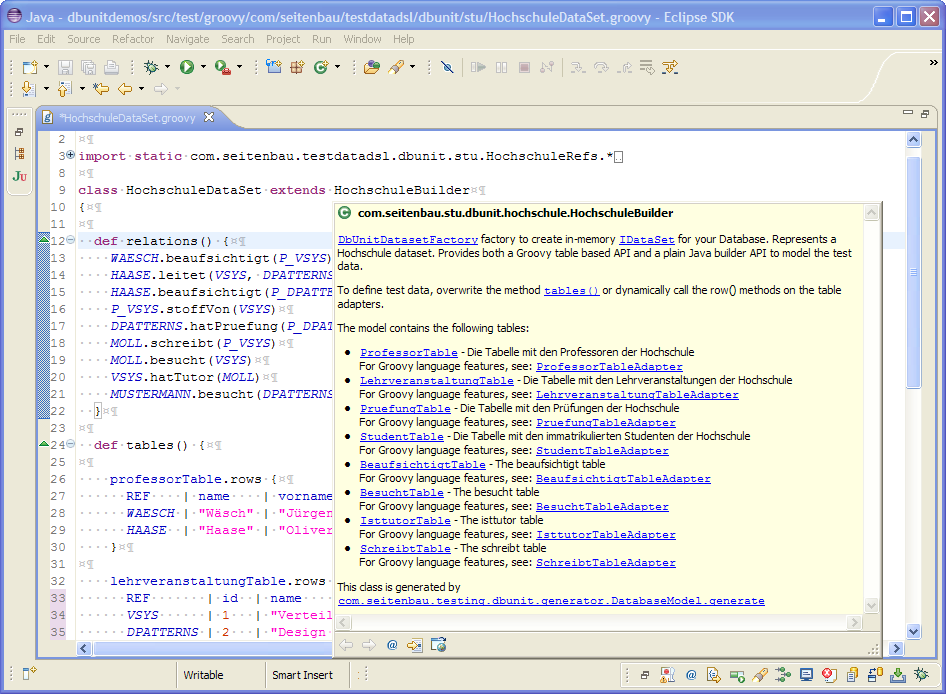
\includegraphics[scale=0.4]{images/realisierung/javadoc_tooltip_builder.png}
	\caption{Tooltip Builder}\label{img:javadoc_tooltip_builder}
\end{figure}

\begin{figure}[H]
	\centering
	 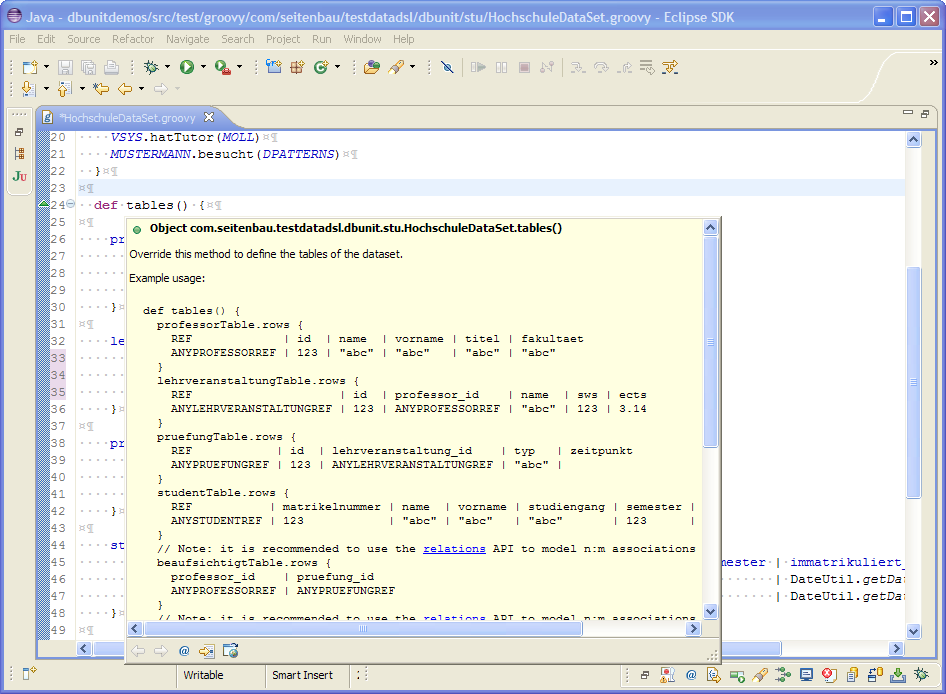
\includegraphics[scale=0.4]{images/realisierung/javadoc_tooltip_tables.png}
	\caption{Tooltip tables()}\label{img:javadoc_tooltip_tables}
\end{figure}

\begin{figure}[H]
	\centering
	 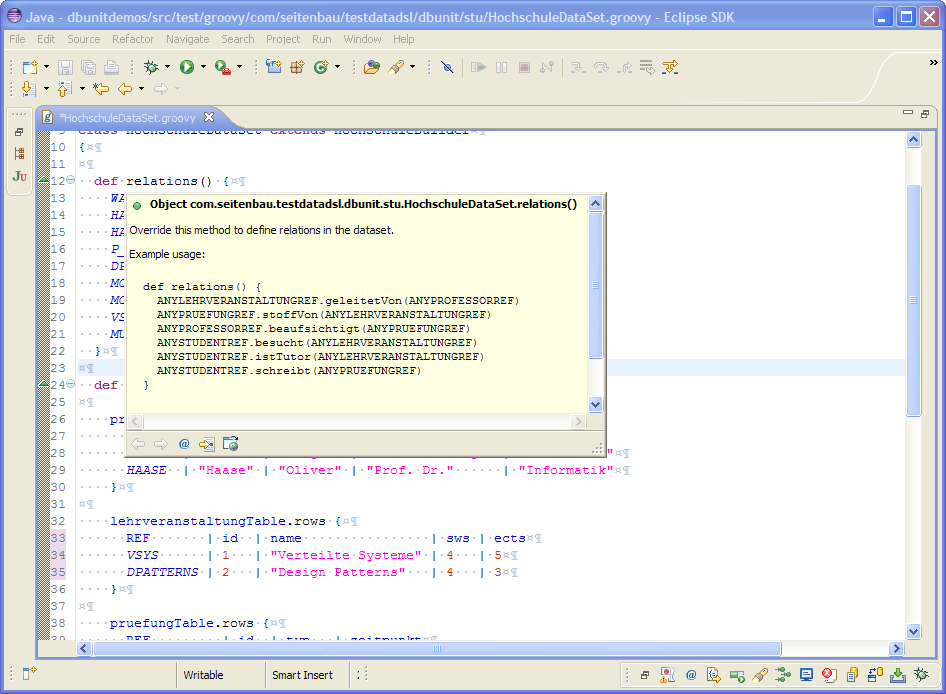
\includegraphics[scale=0.4]{images/realisierung/javadoc_tooltip_relations.png}
	\caption{Tooltip relations()}\label{img:javadoc_tooltip_relations}
\end{figure}

\begin{figure}[H]
	\centering
	 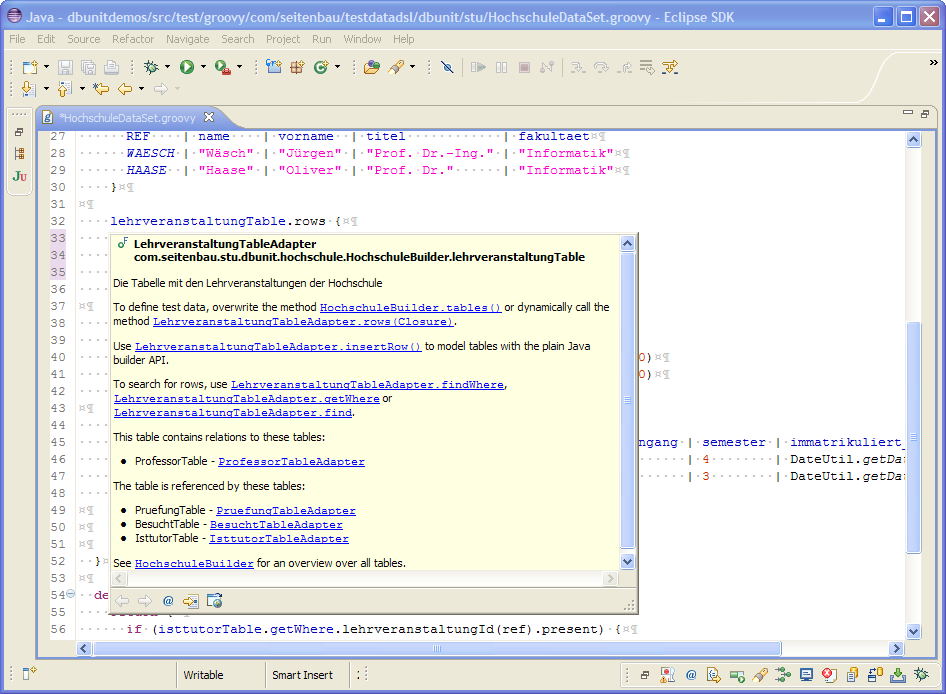
\includegraphics[scale=0.4]{images/realisierung/javadoc_tooltip_table.png}
	\caption{Tooltip Tabelle}\label{img:javadoc_tooltip_table}
\end{figure}

\begin{figure}[H]
	\centering
	 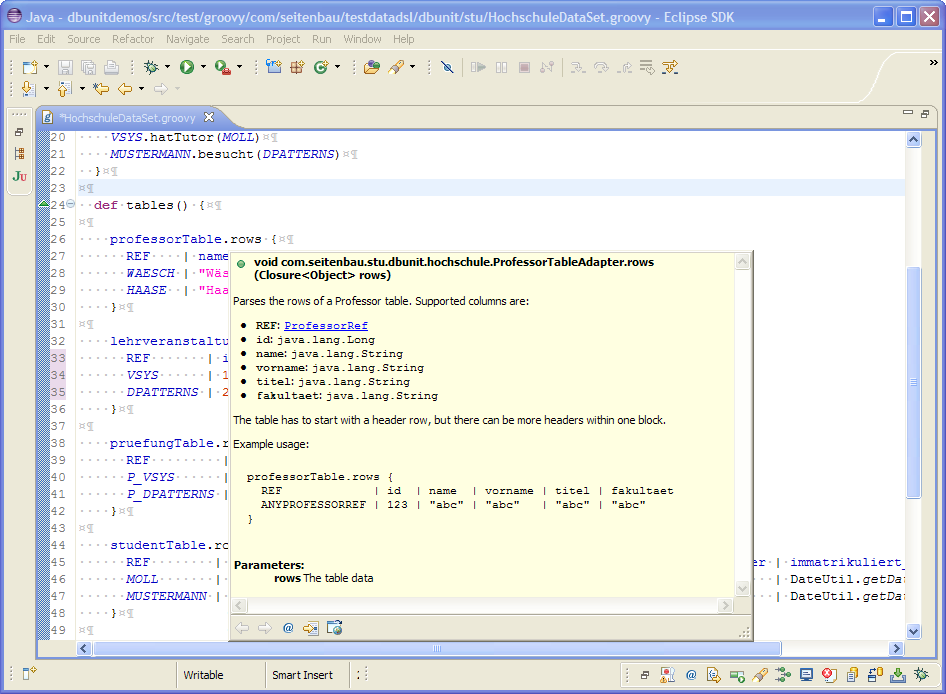
\includegraphics[scale=0.4]{images/realisierung/javadoc_tooltip_rows.png}
	\caption{Tooltip Zeilen}\label{img:javadoc_tooltip_rows}
\end{figure}


  \subsection{Nicht umgesetzt}
	\label{sec:modellierung:realisierung:nichtumgesetzt}
	
	Die Realisierung k�nnte an manchen Stellen dem Test-Ingenieur mehr manuelle Arbeit abnehmen. So wird darauf verzichtet,
	beim L�schen einer Zeile aus einer Tabelle auch alle beteiligten Beziehungen zu entfernen. Listing \ref{listing:deleteexample}
	zeigt, wie ein Professor aus der Professoren-Tabelle entfernt wird. Die erste Zeile entfernt keine Eintr�ge in 
	anderen Tabellen wie z.B. der Beaufsichtigt-Tabelle. Folglich m�ssen die Relationen (mehr oder weniger) manuell
	aus anderen Tabellen entfernt werden.

  \begin{lstlisting}[caption=L�schen von Zeilen, label=listing:deleteexample]
dataSet.professorTable.deleteRow(HAASE);
dataSet.beaufsichtigtTable.deleteAllAssociations(HAASE);
  \end{lstlisting}
	
	Diese Entscheidung hat unterschiedliche Gr�nde:
	\begin{itemize}
		\item \textbf{Einsatzgebiet}: Die Bibliothek soll Unit-Tests in Verbindung mit Datenbanken vereinfachen. Es handelt sich
		  hier nicht um ein API, das in einer Anwendung ausgeliefert wird. W�hrend es in einem API f�r produktive Anwendungen
			durchaus w�nschenswert sein kann, dass das System beim L�schen von Entit�ten gewisse Aufgaben automatisch erledigt,
			ist so ein Verhalten innerhalb einer Test-Bibliothek zweifelhaft. Explizites L�schen von Zeilen auf allen beteiligten
			Tabellen verbessert die Ausdrucksst�rke des Tests.
			
		\item \textbf{Code-Qualit�t}: Nach Robert C. Martin soll eine Funktion (bzw. Methode) genau eine Aufgabe erledigen. Wenn
		  \texttt{deleteRow} zus�tzlich beteiligte Relationen aufl�st, erledigt diese Funktion mehr als nur eine Aufgabe 
			\cite[65f]{CLEAN_CODE}. Au�erdem w�rde es sich um einen unerwarteten Nebeneffekt handeln \cite[75f]{CLEAN_CODE}.
		
		\item \textbf{Klarheit}: Es ist nicht eindeutig, wie beim Entfernen von Zeilen vorgegangen werden soll, wenn sie
		  Teil einer Relation sind. Bei einer n:m-Relation k�nnte sich die Regel ableiten lassen, dass beim L�schen einer
			Zeile auch alle assoziierten n:m-Relationen entfernt werden k�nnen. Aber was ist bei einer 1:n-Relation? Wenn
			ein Professor entfernt wird, was soll mit Lehrveranstaltungen passieren, die ihm zugeordnet sind?
	\end{itemize}

  
		
\todo{"`Muster"' f�r 1:1, 1:n und m:n}

	\chapter{Realisierung der Sprache}
\label{chap:realiserungdsl}

Das folgende Kapitel beschreibt die Implementierung der in Kapitel \ref{chap:modellierung} entwickelten Sprache.
\textit{STU} stellt die Basis f�r Erweiterungen und Verbesserung dar. Es verfolgt bereits das Ziel, Tests von
Datenbank-basierten Anwendungen zu erleichtern und vereinfacht die Modellierung von DbUnit-DataSets. Auf Abw�rtskompatibilit�t
wird wenn notwendig zu Gunsten der Benutzbarkeit und Wartbarkeit verzichtet.

Aus einem dom�nenspezifischen Datenbank-Modell erzeugt \textit{STU} ein individuelles API zur Modellierung von DataSets.
Um die Modellierung zu vereinfachen, vor allem in Bezug auf die Beziehungen, sollen die generierten Klassen um eine Fassade
erg�nzt werden. 

Eine M�glichkeit, eine solche Fassade zu realisieren, stellen dom�nenspezifische Sprachen dar. Eine dom�nenspezifische
Sprache zeichnet sich dadurch aus, dass sie f�r ein spezielles Problemfeld entworfen wurde. Martin Fowler erkl�rt in
\cite[xix]{DOMAIN_SPECIFIC_LANGUAGES}, dass die meisten dom�nenspezifischen Sprachen lediglich eine d�nne Fassade �ber
einer Bibliothek oder einem Framework sind.

Der Code-Generator aus \textit{STU} erzeugt zwei APIs f�r die Modellierung von DataSets:
\begin{itemize}
  \item Das \textbf{Fluent Builder API} ist ein \textbf{Java}-basiertes API. Der Name spiegelt wider, dass es ein Java
    Fluent API bereit stellt (siehe auch Abschnitt \ref{sec:grundlagen:stu}). Ein solches API wird auch als
    interne DSL bezeichnet.
      
  \item Das \textbf{Table Builder API} ist das \textbf{Groovy}-basierte API bzw. die neue DSL. �ber diese DSL k�nnen
    die Testdaten tabellarisch modelliert werden.
      
\end{itemize}

Abbildung \ref{img:architektur} stellt die Architektur eines Tests grafisch dar. Der Test basiert auf 
einem Test-Framework wie \textit{JUnit}, der Testbibliothek \textit{STU} und der Bibliothek \textit{DbUnit}.
\textit{STU} setzt sich aus den beiden oben genannten Schichten zusammen.

\begin{figure}[htbp]
  \centering
   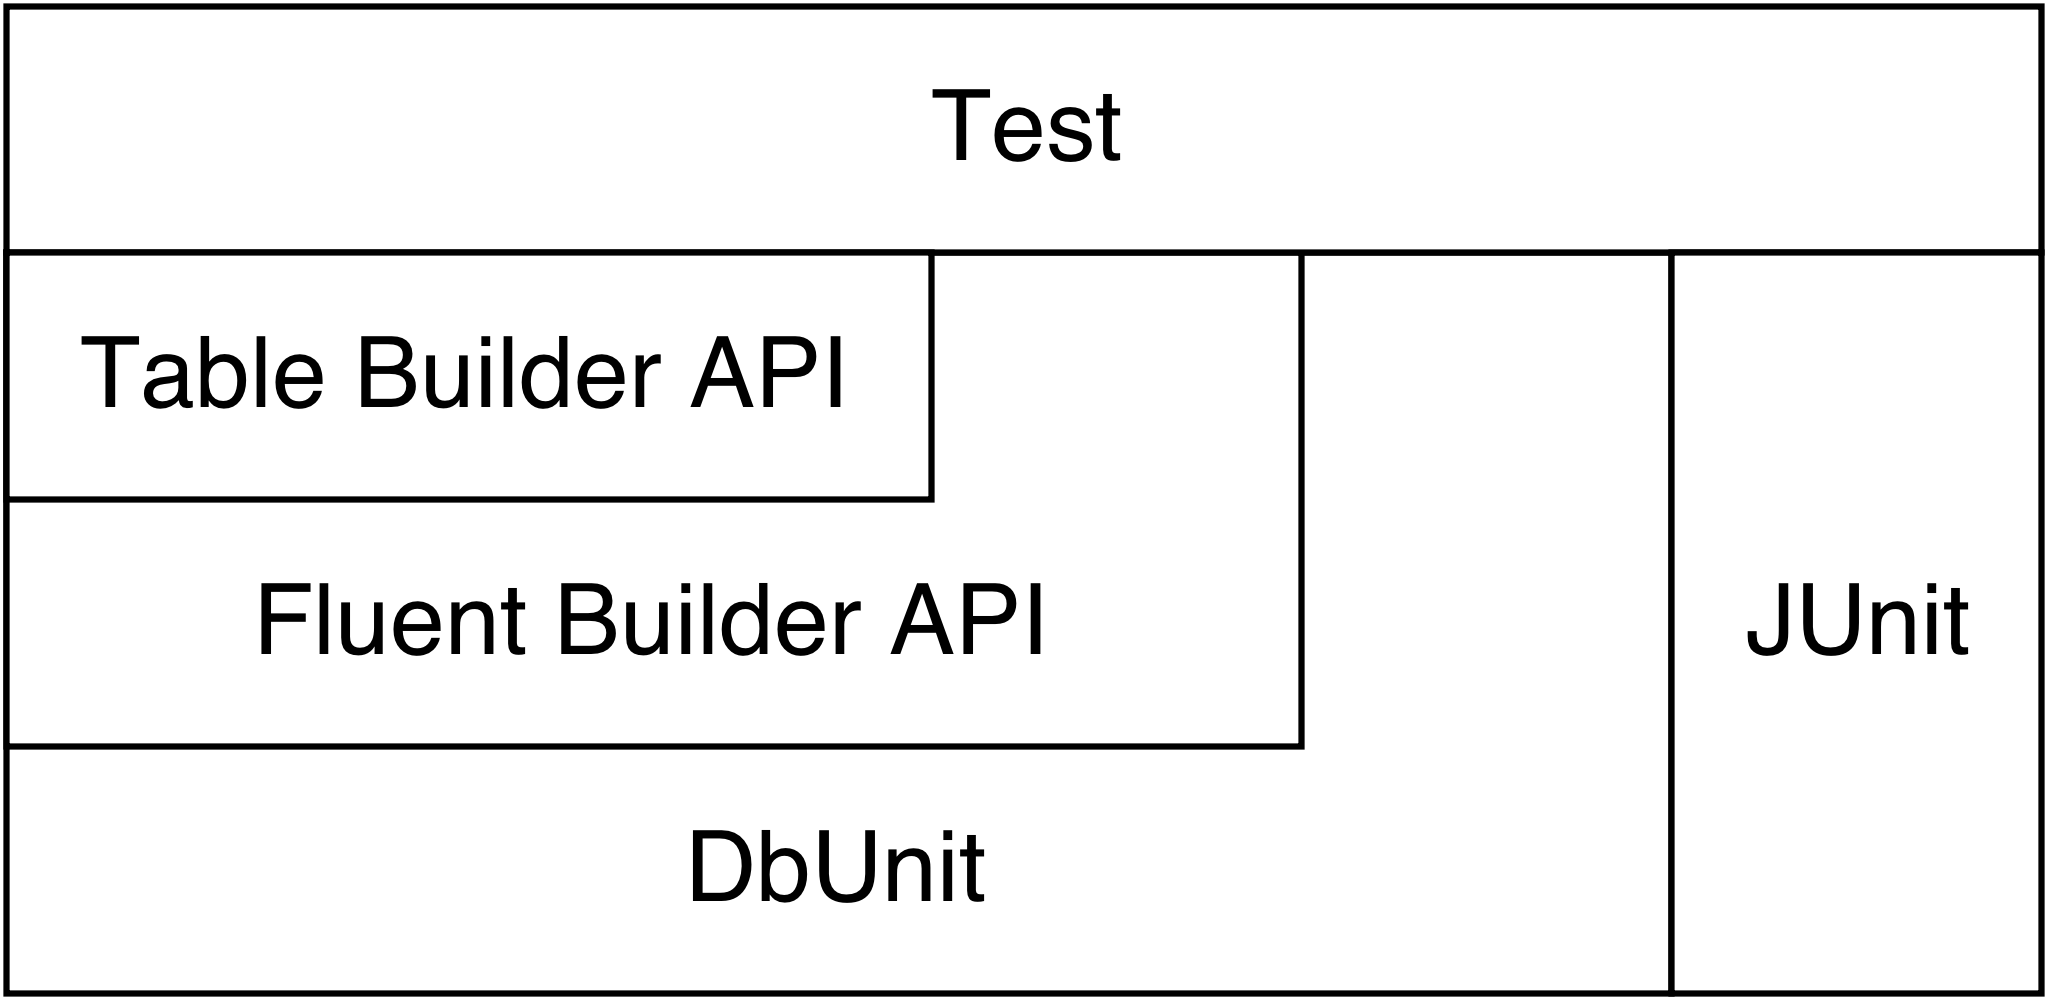
\includegraphics[width=0.43\textwidth]{images/realisierung/stu_architektur.png}
  \caption{Architektur}\label{img:architektur}
\end{figure}

Das neue Table Builder API stellt eine Schicht �ber dem bisherigen Fluent Builder API dar. Neue Funktionen m�ssen 
jedoch nicht zwangsl�ufig im Table Builder API hinzugef�gt werden, unter Umst�nden kann es vorteilhaft sein, sie
direkt in das Fluent Builder API zu integrieren. Gr�nde daf�r sind unter anderem:
\begin{itemize}
  \item \textbf{Code-Qualit�t}: Die neuen Funktionen k�nnen direkt in bestehende Klassen integriert werden, anstatt
    neue Typen einzuf�hren. Auf Adapter-Klassen und Delegation kann auf diese Weise verzichtet werden. Das erleichtert
		die Pflege der Implementierung und vermeidet redundanten Code.
      
  \item \textbf{Mehrwert auch f�r bisheriges API}: Auch wenn auf das neue Table Builder API verzichtet wird,
    kann das Builder API so einen Mehrwert gegen�ber der bisherigen \textit{STU}-Implementierung bieten.
		Verbesserungen im Fluent Builder API sind auch in reinen Java-basierten Tests nutzbar.
      
  \item \textbf{Einheitlicher Funktionsumfang}: Das Table Builder API und das Fluent Builder API sollen -- so weit
	  m�glich und sinnvoll -- denselben Funktionsumfang bieten. Erweiterungen f�r das Fluent Builder API stehen
		automatisch auch im Table Builder API zur Verf�gung.

\end{itemize}




\section{�nderungen am Generator-Modell}
\label{sec:modellierung:generatormodell}

  Die hinzugekommenen Funktionen erfordern Erweiterungen in den Klassen zur Modellierung der zugrunde liegenden Datenbank.
  Das bisherige API in \textit{STU} nutzt �berladene Methoden mit vielen optionalen Parametern zur Beschreibung von Spalten.
	Dies ist weder wartungs- noch anwenderfreundlich. Jeder neue optionale Parameter w�rde die Anzahl der Methoden unter
	Umst�nden verdoppeln. F�r Anwender ist es nicht immer einfach, sich die Reihenfolge langer Parameterlisten zu merken,
	v.a. wenn es mehrere Varianten derselben Methode gibt.
	
	Die Klassen zur Beschreibung des Generator-Modells werden deshalb auf das Builder-Pattern umgestellt. Dieses l�st beide
	Probleme. Jeder zus�tzliche optionale Parameter f�hrt zu einer neuen Methode. Die Reihenfolge der Methodenaufrufe ist im
	Gegensatz zu Parameterlisten beliebig. Der Code liest und schreibt sich einfacher, da Parameter durch die Methodenaufrufe
	benannt sind.
  
  Die neuen Builder-Klassen decken den Funktionsumfang des alten API ab. Dabei werden Eigenschaften f�r Spalten nicht mehr �ber 
  ein \texttt{EnumSet} festgelegt, sondern �ber Methoden f�r die vordefinierten Flags. In Abschnitt 
  \ref{sec:modellierung:generatormodell:flags}  wird weiter auf das Thema Flags eingegangen. Dar�ber hinaus bieten die
  neuen Klassen die M�glichkeit, Beschreibungen zu Tabellen und Spalten hinzuzuf�gen. Diese werden bei der Code-Generierung
  f�r die Erstellung von JavaDoc-Kommentaren verwendet (\refsec{sec:ralisierungdsl:javadoc}).
  
	Erweiterungen am Generator-Modell betreffen vor allem die Modellierung von Beziehungen zwischen Tabellen. Der folgende Abschnitt
	beschreibt die Modellierungskonzepte f�r Beziehungen in Datenbanken.


  
  \subsection{Spalten-Eigenschaften}
  \label{sec:modellierung:generatormodell:flags}
  
	Meta-Informationen von Spalten beinhalten neben dem Namen der Spalte und dem Typ weitere Eigenschaften. Diese Eigenschaften
	werden in \textit{STU} mit Hilfe sogenannter Flags beschrieben. Die Flags sind bislang in einem \textit{Enum}
	zusammengefasst. Alle f�r eine Spalte gesetzten Flags m�ssen beim Hinzuf�gen einer Spalte �ber ein \textit{EnumSet}
  �bergeben werden. Bei dem neuen Builder-API werden die Flags �ber spezielle Methoden gesetzt.
  
  Zu den in \textit{STU} enthaltenen Standard-Spalten-Flags geh�ren:
  \begin{itemize}
    \item \textbf{Identifier}: Dieses Flag gibt an, dass die Werte einer Spalte die Zeile eindeutig identifizieren. 
      Sollen Werte in einer Zeile abgefragt oder ver�ndert werden, kann die Zeile mit Hilfe einer solchen Spalte 
      identifiziert werden.
       
      Da die Werte zur Identifikation verwendet werden, ist ein nachtr�gliches �ndern nicht erlaubt. Dies soll anhand eines
      kurzen Beispiels begr�ndet werden (siehe Listing \ref{listing:beispielimmutable}). Es zeigt einen Ausschnitt einer
      Studenten-Tabelle. Die Spalten \texttt{id} und \texttt{matrikelnummer} sind mit dem Flag \texttt{Identifier}
      versehen. In Zeile 2 werden Daten mit der ID 1 und der Matrikelnummer 123456 definiert. Zeile 3 steht f�r beliebige
      Anweisungen, in Zeile 4 und 5 wird die Studententabelle erweitert, z.B. innerhalb eines Unit-Tests. Zeile 5
      definiert Daten mit der ID 2 und der vorherigen Matrikelnummer. Beziehen sich beide Zeilen auf 
      denselben Studenten und die ID soll ver�ndert werden? Oder wurde die Matrikelnummer irrt�mlich falsch angegeben?
      Die ID des Studenten Mustermann auf 2 zu �ndern, k�nnte zu Problemen f�hren, da nicht bekannt ist, an welchen Stellen
      bereits auf ID 1 Bezug genommen wird.
      
      \begin{lstlisting}[caption=Beispiel f�r unver�nderliche Identifikatoren, label=listing:beispielimmutable]
id | matrikelnummer | Name      
1  | 123456         | "Mustermann" 
...
id | matrikelnummer | vorname 
2  | 123456         | "Nikolaus"       
      \end{lstlisting}
      
      
      Das Flag wird �ber die Methode \texttt{identifier()} gesetzt, dabei wird das Flag \texttt{Immutable} implizit aktiviert.

    \item \textbf{Default Identifier}: Dieses Flag stellt eine Art Erweiterung f�r das Flag \texttt{Identifier} dar. Die mit
      diesem Flag markierte Spalte wird f�r Foreign-Key-Beziehungen auf die Tabelle verwendet, sofern nicht explizit eine
      andere Spalte angegeben wird. Die Methode zum Setzen des Flags ist \texttt{defaultIdentifier()}, die Flags \texttt{Identifier}
      und \texttt{Immutable} werden automatisch aktiviert.
      
    \item \textbf{Add Next Method}: \textit{STU} bietet die M�glichkeit, Werte-Generatoren 
      zu verwenden, um einen Spaltenwert manuell oder auch automatisch mit einem generierten Wert zu belegen. Aufgerufen wird der 
      Generator �ber eine sogenannte Next-Value-Methode auf dem RowBuilder. Ihr Name setzt sich aus dem Pr�fix \texttt{next} und dem
      Spaltennamen zusammen. Der Generator erzeugt f�r die jeweilige Spalte allerdings nur dann eine Next-Value-Methode, wenn das
      entsprechende Flag �ber \texttt{addNextMethod()} aus dem Builder-API gesetzt wurde. Standardm��ig muss die Next-Value-Methode
      manuell aufgerufen werden, �ber ein Flag kann dies auch automatisch erfolgen.
      
    \item \textbf{Auto Invoke Next}: Ist dieses Flag aktiviert, wird die Next-Value-Methode beim 
      Anlegen einer neuen Tabellenzeile automatisch aufgerufen. Beim Setzen des Flags �ber die Builder-Methode
      \texttt{autoInvokeNext()} wird automatisch auch das Flag zum Generieren der Next-Value-Methode gesetzt. 
    
    \item \textbf{Immutable}: Ist dieses Flag gesetzt, kann ein Wert in einer Spalte nur ein Mal gesetzt und danach
      nicht mehr ver�ndert werden. Wenn das Flag zum automatischen Aufruf der Next-Value-Methode aktiviert ist, kann der
      automatisch erzeugte Wert allerdings �berschrieben werden. Die Methode zum
      Aktivieren des Flags hei�t \texttt{immutable()}.
      
    %\item \textbf{Auto Increment}: ... DBUNIT-Flag ... implizit addNextMethod
      
  \end{itemize}


  
  \subsection{Modellierung von Relationen �ber Builder-Klassen}
  \label{sec:modellierung:generatormodell:relationen}
  
  Das API zur Modellierung des Datenbankschemas als Grundlage f�r den Generator stellt eine der gr��ten Ver�nderungen
	in der Implementierung dar. Die gr��ten �nderungen betreffen  die Definition von Beziehungen zwischen Tabellen.
	�ber \texttt{reference} kann der Builder zur Beschreibung der Relation aufgerufen werden. Die Beschreibung findet
	in zwei Bereichen statt:
  
  \begin{itemize}
    \item \textbf{local}: Der als \texttt{local} bezeichnete Teil beschreibt die Beziehung aus Sicht der Tabelle,
      in der sich die Spalte befindet. 
      
    \item \textbf{foreign}: Der \texttt{foreign}-Teil dient der Beschreibung der Beziehung aus Sicht der Tabelle,
      mit der die Beziehung hergestellt wird.
    
  \end{itemize}
  
  In beiden Bereichen kann ein Bezeichner angegeben werden. Dieser Bezeichner dr�ckt die Beziehung in die
	jeweilige Richtung aus, in \textit{local} wird die Beziehung in Richtung \textit{foreign} bezeichnet. 
	Diese Bezeichner werden f�r die Methoden zur Modellierung der Beziehungen verwendet. Daneben k�nnen
	auch noch Beschreibungstexte angegeben werden, die f�r die JavaDoc genutzt werden.
  
  In Abschnitt \ref{sec:modellierung:generatormodell:buildervergleich} befindet sich ein Beispiel f�r die 
  Modellierung von Relationen.
  
  Durch die Nutzung des Builder-Patterns lassen sich weitere Attribute verh�ltnism��ig einfach hinzuf�gen, z.B.
  f�r die Generierung der Testdaten (siehe Kapitel \ref{chap:generieren}).
  
  
  \subsection{Alte und neue Builder-Klassen im Vergleich}
  \label{sec:modellierung:generatormodell:buildervergleich}
  
  Die Vorteile der Umstellung auf das Builder-Pattern sollen die beiden folgenden Listings veranschaulichen. Sie zeigen
  die Modellierung der Datenbank f�r den Generator. Der �bersicht halber wurde der Code auf die Anweisungen
  im Konstruktor der Modell-Klasse und die Definition von zwei Tabellen reduziert. Listing 
  \ref{listing:model:builder:old} zeigt die Modellierung im urspr�nglichen \textit{STU}, w�hrend Listing
  \ref{listing:model:builder:new} die neuen Builder darstellt.
  
  \begin{lstlisting}[caption=Beispiel alte \textit{STU}-Builder, label=listing:model:builder:old]
database("Hochschule");
packageName("com.seitenbau.testing.dbunit.hochschule");

Table professoren = addTable("professor")
    .addColumn("id", DataType.BIGINT, Flags.AutoInvokeNextIdMethod) 
    .addColumn("name", DataType.VARCHAR)
    .addColumn("vorname", DataType.VARCHAR)
    .addColumn("titel", DataType.VARCHAR)
    .addColumn("fakultaet", DataType.VARCHAR);

Table lehrveranstaltungen = addTable("lehrveranstaltung")
    .addColumn("id", DataType.BIGINT, Flags.AutoInvokeNextIdMethod)
    .addColumn("professor_id", DataType.BIGINT, professoren.ref("id"))
    .addColumn("name", DataType.VARCHAR)
    .addColumn("sws", DataType.INTEGER)
    .addColumn("ects", DataType.DOUBLE);
  \end{lstlisting}
  
  In diesem Beispiel -- inkl. der nicht dargestellten Tabellen-Definitionen -- werden lediglich drei der
  insgesamt neun \texttt{addColumn}-Methoden verwendet.
  
  Die Codes zur Modellierung mit der alten und der neuen API �hneln sich, die Unterschiede liegen abgesehen
  von den Flags und Relationen eher im Detail. Listing \ref{listing:model:builder:new} zeigt die Modellierung
  derselben Tabellen mit dem neuen API. Die k�rzeren Parameterlisten und die zus�tzlichen Funktionen f�hren
  dazu, dass dieselben Modelle in \textit{STU} einige Zeilen l�nger werden. Dieser Nachteil wird durch
	die gewonnene Ausdrucksst�ke mehr als ausgeglichen.
  
  \begin{lstlisting}[caption=Beispiel neue \textit{STU}-Builder, label=listing:model:builder:new]
database("Hochschule");
packageName("com.seitenbau.testing.dbunit.hochschule");

Table professoren = table("professor")
    .description("Die Tabelle mit den Professoren der Hochschule")
    .column("id", DataType.BIGINT) 
      .identifierColumn() 
      .autoInvokeNext()
    .column("name", DataType.VARCHAR)
    .column("vorname", DataType.VARCHAR)
    .column("titel", DataType.VARCHAR)
    .column("fakultaet", DataType.VARCHAR)
  .build();

Table lehrveranstaltungen = table("lehrveranstaltung")
    .description("Die Tabelle mit den Lehrveranstaltungen der Hochschule")
    .column("id", DataType.BIGINT)
      .identifierColumn() 
      .autoInvokeNext()
    .column("professor_id", DataType.BIGINT)
      .reference
        .local
          .name("geleitetVon")
          .description("Gibt an, von welchem Professor eine Lehrveranstaltung geleitet wird.")
        .foreign(professoren)
          .name("leitet")
          .description("Gibt an, welche Lehrveranstaltungen ein Professor leitet.")
    .column("name", DataType.VARCHAR)
    .column("sws", DataType.INTEGER)
    .column("ects", DataType.DOUBLE)
  .build();  
  \end{lstlisting}

    
	Bei der Modellierung von n:m-Beziehungen kann auf den \texttt{local}-Teil der Beziehung verzichtet werden.
	\textit{STU} verwendet automatisch den \texttt{foreign}-Teil der assoziierten Spalte. Anstelle der Methode
	\texttt{table} wird eine assoziative Tabelle mit der Methode \texttt{associativeTable} beschrieben. Listing
	\ref{listing:model:builder:assoc} zeigt ein Beispiel f�r die Modellierung einer assoziativen Tabelle:

  \begin{lstlisting}[caption=Beispiel f�r assoziative Tabelle, label=listing:model:builder:assoc]
associativeTable("besucht")
  .column("student_id", DataType.BIGINT)
    .reference
      .foreign(studenten)
        .name("besucht")
        .description("Die Lehrveranstaltungen, die ein Student besucht.")
  .column("lehrveranstaltung_id", DataType.BIGINT)
    .reference
      .foreign(lehrveranstaltungen)
        .name("besuchtVon")
        .description("Die Studenten, die eine Lehrveranstaltung besuchen.")
 .build();
  \end{lstlisting}



  \section{Neue DataSet-Builder-Klassen}
  \label{sec:realisierung:neuebuilder}
  
  F�r die tabellarisch definierten DataSets wird eine neue Builder-Klasse generiert, die �ber Komposition und Delegation die
  bisherige, auf dem Fluent-Builder-API-basierende DataSet-Klasse nutzt.

  Der Gro�teil des IDE-Supports wird �ber Adapter-Klassen f�r die bisherigen Tabellen realisiert \cite[139]{DESIGN_PATTERNS}.
	Zu jeder Tabellen-Klasse wird
  eine zus�tzliche Adapter-Klasse generiert. Dort sind die Tabellen-spezifischen Spaltenbezeichner f�r die tabellarische DSL
  definiert. Die Methode \texttt{rows} startet das Parsen der Tabellenzeilen, die wie im Entwurf als Closure �bergeben werden.
  Innerhalb dieses Closures sind die in der Tabelle definierten Bezeichner nutzbar. Neben den Spaltenbezeichnern werden ein
  Spaltenbezeichner \texttt{REF} und auch der Platzhalter (Unterstrich) generiert. Die Adapter nutzen intern eine aggregierte
  Tabellen-Klasse. Dabei bildet der Adapter die Schnittstelle der Tabellen-Klasse nach und delegiert die Aufrufe.
  
  Jeder Spaltenbezeichner stellt eine anonyme Klasse dar, die die abstrakte Klasse \texttt{ColumnBinding} erweitert. Diese 
  enth�lt Meta-Informationen zu der zugeh�rigen Spalte und Methoden, die das Parsen der Tabellen erleichtern
  (siehe Abschnitt \ref{sec:ralisierungdsl:parser}). 

  F�r jede Tabelle gibt es in der Builder-Klasse eine �ffentliche Instanz der Adapter-Klasse. Auf diese Weise wird der
  IDE-Support bzgl. der Tabellennamen sichergestellt. Das Klassendiagramm ist in Abbildung \ref{img:builderarchitecture} dargestellt.

  \begin{figure}[htbp]
    \centering
     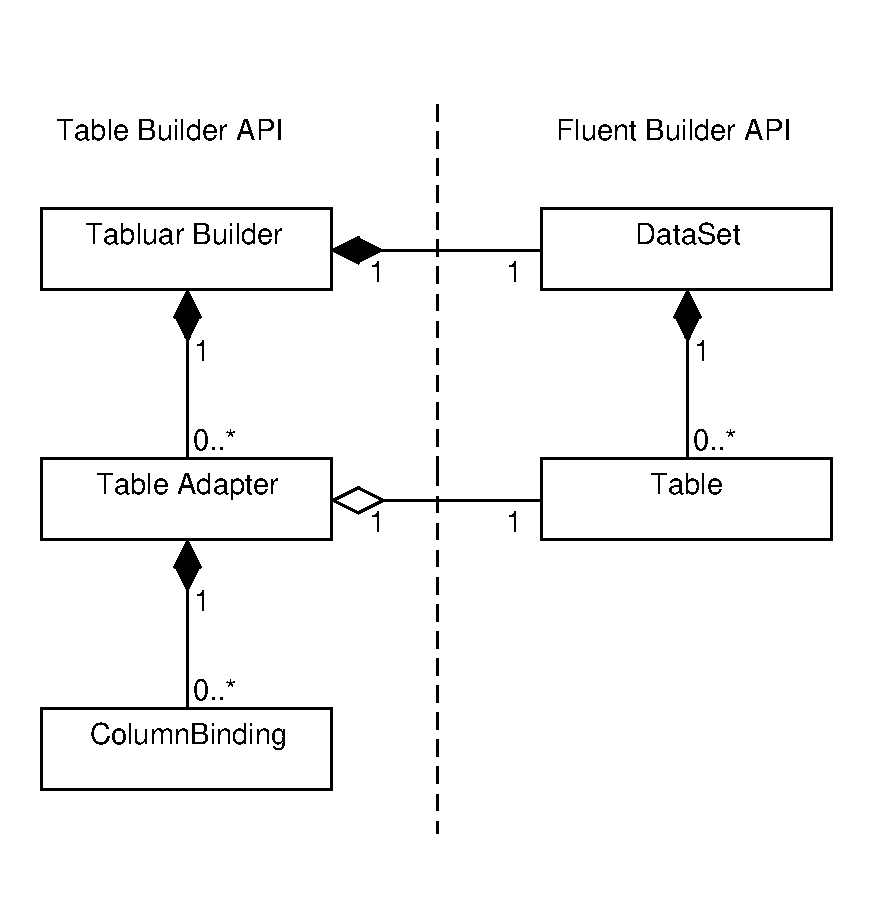
\includegraphics[width=0.6\textwidth]{images/realisierung/builderarchitecture.pdf}
    \caption{Klassendiagramm der DataSet-Builder}\label{img:builderarchitecture}
  \end{figure}
  
  
  



% http://martinfowler.com/eaaCatalog/gateway.html
% http://martinfowler.com/eaaCatalog/repository.html
% http://martinfowler.com/eaaCatalog/registry.html

    
  \section{Tabellenparser}
  \label{sec:ralisierungdsl:parser}
  
  F�r den Parser wird der Code aus dem Prototyp genutzt (siehe Abschnitt \ref{sec:modellierung:implementierung:varianten:laufzeit}).
  Die Logik an sich ist relativ generisch, je nach konkreter Tabelle muss allerdings mit unterschiedlichen Datentypen
  gearbeitet werden. 
  
  Folgende zwei M�glichkeiten bieten sich an, den Parser zu realisieren:
  \begin{enumerate}
    \item F�r jede Tabellen-Adapter-Klasse wird individueller Parser-Code generiert.
    \item Die Tabellen-Adapter nutzen eine generische Parser-Klasse.
  \end{enumerate}

  Die Generierung von redundantem Code scheint kein gro�er Nachteil zu sein. Gerade bei generiertem Code wird Redundanz weniger
  kritisch gesehen. Allerdings erreicht der Code zum Parsen einer Tabelle eine gewisse Komplexit�t, die die Pflege des Codes
  auf Template-Ebene erschwert. Die generische Klasse ist etwas aufw�ndiger zu implementieren, hat aber einige Vorteile: Die Wartung
  erfolgt IDE-unterst�tzt und �nderungen erfordern in der Regel keine Neu-Generierung der Tabellen-Klassen. F�r die Tester
  ist der gr��te Vorteil jedoch, dass keine der zu generierenden Klassen spezielle Groovy-Features nutzen muss und es damit 
  ausreicht, Java-Klassen zu verwenden.
  
  Die Schwierigkeiten, die mit der Entscheidung zugunsten des generischen Parsers gel�st werden m�ssen, betreffen Operationen,
  die der Parser auf der Tabelle durchf�hren muss: Anlegen neuer Zeilen, Suchen nach Zeilen und Setzen von Werten auf den Zeilen.
  Dies wird unter anderem mit einem weiteren Adapter zwischen den bereits bekannten Table-Adapter-Klassen und dem generischen
  Table-Parser erreicht. Dieser Adapter implementiert das Interface \texttt{TableParserAdapter}. Die 
  Typ-Parameter enthalten Informationen zu den konkret verwendeten Klassen wie dem RowBuilder. Dar�ber hinaus bietet die Schnittstelle
  die ben�tigten Methoden zum Erstellen und Suchen von Tabellen-Zeilen.

  Das Setzen der Werte auf den RowBuildern ist deshalb ein Problem, weil die Bezeichner der Set-Methoden die Spaltennamen enthalten.
  Eine L�sung ist die bereits im letzten Abschnitt angesprochene \texttt{ColumnBinding}-Klasse. Sie definiert die abstrakte
  generische Methode \texttt{set(R row, Object value)}, wobei \texttt{R} der Typ-Parameter f�r den RowBuilder ist.
  In die Implementierungen der \texttt{set}-Methoden kann der korrekte Bezeichner f�r den jeweiligen Setter auf dem RowBuilder
  generiert werden.
  
	Mit automatischen Typumwandlungen bietet \texttt{STU} eine Komfortfunktion, die die Lesbarkeit weiter verbessert.
	Vom Parser eingelesene Werte werden nach M�glichkeit automatisch in den vom Modell erwarteten Datentyp konvertiert.
	Diese Konvertierung ist notwendig, da alle eingelesenen Werte als Objekte und nie als primitive Datentypen vorliegen.
	Beispielsweise konvertiert der Parser ein \texttt{Integer}-Wert in einer Spalte f�r \texttt{Double}-Werte in den
	passenden Typ. 
  
  \section{Referenzen und Scopes}
  \label{sec:ralisierungdsl:refs_and_scopes}
  
  Neben der M�glichkeit, Daten tabellarisch zu modellieren, geh�ren die neuen Referenz-Datentypen zu der wichtigsten Erweiterung.
  In \textit{STU} ist eine Referenz eine Art Stellvertreter f�r eine Entit�t (Tabellenzeile). Die Referenz kann bei der Modellierung 
  oder auch bei Such-Anfragen anstelle konkreter Werte (wie Prim�rschl�ssel) verwendet werden. Die Such-Anfrage-M�glichkeiten
  werden in Abschnitt \ref{sec:ralisierungdsl:apierweiterungen} erl�utert. Eine Referenzen werden im Folgenden auch als Ref bezeichnet.
  
  Referenzen m�ssen an ihre Datens�tze gebunden werden. Im Table Builder API ist daf�r die Spalte \texttt{REF} vorgesehen,
  die in jeder Tabelle genutzt werden kann, das Fluent Builder API bietet auf den RowBuilder-Klassen die Methode \texttt{bind()}.
  Die Listings \ref{listing:ref:bindingtable} und \ref{listing:ref:bindingfluent} zeigen die Modellierung derselben Zeile 
  einmal mit dem neuen Table Builder API und einmal mit dem erweiterten Fluent Builder API.
  
  \begin{lstlisting}[caption=Binden von Referenzen (Table Builder API), label=listing:ref:bindingtable]
professorTable.rows {
  REF    | name    | vorname  | titel            | fakultaet
  WAESCH | "W�sch" | "J�rgen" | "Prof. Dr.-Ing." | "Informatik"
  ...
}
  \end{lstlisting}
  
  \begin{lstlisting}[caption=Binden von Referenzen (Fluent Builder API), label=listing:ref:bindingfluent]
table_Professor.insertRow()
  .bind(WAESCH)
  .setName("W�sch")
  .setVorname("J�rgen")
  .setTitle("Prof. Dr.-Ing.")
  .setFakultaet("Informatik")
...
  \end{lstlisting}
  
  Da Referenzen die zugeh�rigen RowBuilder kennen, k�nnen ihre Werte auch direkt auf der Referenz abgefragt werden 
  (\reflst{listing:ref:valueaccess}).
  
  \begin{lstlisting}[caption=Zugriff auf Werte �ber Referenzen, label=listing:ref:valueaccess]
WAESCH.getName()    // Java style
WAESCH.name         // Groovy style
  \end{lstlisting}
  
  Dar�ber hinaus k�nnen �ber Referenzen Beziehungen modelliert werden. Sie enthalten Methoden zum Ausdr�cken von Beziehungen.
  Die Methodennamen entsprechen den im Generator-Modell angegebenen Relationsnamen. Listing \ref{listing:ref:relations} zeigt
	anhand eines Beispiels, wie Beziehungen �ber Referenzen definiert werden.
	
  \begin{lstlisting}[caption=Definition von Beziehungen �ber Referenzen, label=listing:ref:relations]
WAESCH.beaufsichtigt(P_VSYS)
  \end{lstlisting}
  
  Die Referenzen m�ssen vor ihrer Nutzung definiert (deklariert und instantiiert) werden. Eine explizite Definition ist
	in Groovy nicht notwendig (siehe Abschnitt~\ref{sec:modellierung:implementierung:varianten:laufzeit}), ist aber 
	f�r die IDE-Unterst�tzung notwendig (z.B. f�r das Umbenennen von Referenzen, Erkennen von Tippfehlern bei Bezeichnern).
	Au�erdem k�nnten sie auch nicht im normalen Java-Code verwendet werden. Es bietet sich an, Referenzen als globale Variablen zu
	definieren. Verschiedene DataSets (mit demselben Datenbank-Modell) k�nnen dieselben Referenzen nutzen, auch wenn sie
	unterschiedliche Werte repr�sentieren.
  
  Damit dieselben Referenzen in unterschiedlichen DataSets genutzt werden k�nnen, werden die RowBuilder immer im Kontext des
  gerade aktiven DataSets gebunden. Das aktive DataSet wird �ber die \texttt{DataSetRegistry} festgelegt (und abgefragt). Pro
  Datenbank-Modell ist immer ein (oder kein) DataSet aktiv. Das hei�t, wenn verschiedene Datenbank-Modelle genutzt werden,
  aus jedem Modell jeweils ein DataSet gleichzeitig aktiv sein kann.
  
  \section{Integration von DataSets in Unit-Tests}
  \label{sec:ralisierungdsl:junittest}
  
  Wie das Beispiel-DataSet aus Listing \ref{listing:hochschuledataset:table} in einem JUnit-Test verwendet werden kann,
  zeigt Listing \ref{listing:junittest}. Das System Under Test (siehe Abschnitt \ref{sec:grundlagen:konzepte:tests})
  ist ein Spring-Service, der von der Variable \texttt{sut} (Zeile 20) repr�sentiert wird.
  
  Das in einem Test verwendete DataSet kann als Klasse �ber die Annotation \texttt{DatabaseSetup} konfiguriert werden
  (Zeile 26). Sie sorgt daf�r, dass die angegebene DataSet-Klasse instantiiert und der Variable zugewiesen wird, die 
  mit der Annotation \texttt{InjectDataSet} markiert wurde (Zeilen 22 und 23). Au�erdem wird dieses DataSet auch bei
  der \texttt{DataSetRegistry} als aktives DataSet registriert und die Daten in die Datenbank eingespielt. Dadurch
  kommen die Test-Methoden ohne Verwaltungsaufgaben aus. Der Test \texttt{removeStudent} testet, ob das System die
  richtigen �nderungen in der Datenbank vornimmt, wenn der Student \texttt{MUSTERMANN} entfernt wird. Da dem Service
  die zu l�schende Entit�t �bergeben werden muss (Zeile 38), wird in den Zeilen 29 bis 35 eine entsprechende Instanz
  erstellt und konfiguriert. 
  
  Der Test verwendet eine \texttt{DatabaseTesterRule} (Zeile 9), die unter anderem f�r die Vergleiche der Datenbank
  mit den DataSets verantwortlich ist. Dazu muss ihr die Datenbank bekannt sein, die in Form einer \texttt{DataSource}
  vorliegt (Zeile 6). Da dieses Feld durch \textit{Dependency Injection} (\cite[4]{PRO_SPRING}) erst
  nach der Instantiierung der Klasse belegt wird, kann bei der Erzeugung von \texttt{dbTester} der Wert noch nicht
  verwendet werden. Dies wird durch die Verwendung eines Future-Objekts gel�st, das die \texttt{DataSource} erst dann
  zur�ckliefert, wenn sie gebraucht wird (Zeilen 10 bis 15). 
  
  \begin{lstlisting}[caption=JUnit-Tests (reiner Java-Code), label=listing:junittest]
@RunWith(SpringJUnit4ClassRunner.class)
@ContextConfiguration(classes=HochschuleContext.class)
public class HochschuleDataSetDatabaseTest {

  @Autowired
  DataSource dataSource;

  @Rule
  public DatabaseTesterRule dbTester =
     new DatabaseTesterRule(new Future<DataSource>(){
       @Override
       public DataSource getFuture()
       {
         return dataSource;
       }
     }).addCleanAction(new ApacheDerbySequenceReset()
       .autoDerivateFromTablename("_SEQ"));

  @Autowired
  HochschuleService sut;

  @InjectDataSet
  HochschuleBuilder dataSet;

  @Test
  @DatabaseSetup(prepare = HochschuleDataSet.class)
  public void removeStudent() throws Exception {
    // prepare
    Student student = new Student();
    student.setMatrikelnummer(MUSTERMANN.getMatrikelnummer());
    student.setVorname(MUSTERMANN.getVorname());
    student.setName(MUSTERMANN.getName());
    student.setStudiengang(MUSTERMANN.getStudiengang());
    student.setSemester(MUSTERMANN.getSemester());
    student.setImmatrikuliertSeit(MUSTERMANN.getImmatrikuliertSeit());

    // execute
    sut.removeStudent(student);

    // verify
    dataSet.studentTable.deleteRow(MUSTERMANN);
    dataSet.besuchtTable.deleteAllAssociations(MUSTERMANN);

    dbTester.assertDataBase(dataSet);
  }
  
  ...

}  
  \end{lstlisting}
  
  In den Zeilen 41 und 42 werden die erwarteten �nderungen im DataSet ebenfalls durchgef�hrt, um in Zeile 44 die
  Datenbank gegen das DataSet zu vergleichen.
  
  Die neue DSL kann in Groovy-basierten Tests verwendet werden. Listing \ref{listing:junittest:groovy} zeigt
  beispielhaft eine entsprechende Test-Methode. In diesem Test wird eine neue Lehrveranstaltung erstellt und
  einem Professor zugeordnet. Die �nderungen am DataSet lassen sich innerhalb der Testmethode mit derselben
	Syntax modellieren.
  
  \begin{lstlisting}[caption=Test-Methode in Groovy, label=listing:junittest:groovy]
  @Test
  @DatabaseSetup(prepare = HochschuleDataSet)
  def addLehrveranstaltung() {
    // prepare
    Lehrveranstaltung lv = new Lehrveranstaltung()
    lv.setName("Programmieren")
    lv.setProfessor(HAASE.id)
    lv.setSws(4)
    lv.setEcts(6.0)

    // execute
    def addedLv = sut.addLehrveranstaltung(lv)

    // verify
    dataSet.lehrveranstaltungTable.rows {
      id         | professor | name            | sws | ects
      addedLv.id | HAASE     | "Programmieren" | 4   | 6.0
    }

    dbTester.assertDataBase(dataSet)
  }
  \end{lstlisting}
  
  Sicherheitshalber wird die vom Service erzeugte ID verwendet, um die �nderungen am Test-DataSet
  durchzuf�hren. Auf diese Weise bleibt der Test stabil, auch wenn sich das Verhalten des Services
  bzw. der Datenbank bei der Vergabe von IDs �ndern sollte.
    
  \section{Komposition von DataSets}
  \label{sec:ralisierungdsl:kompositiondatasets}
  
  DataSets lassen sich aus anderen zusammensetzen. Dieses Feature setzt nicht auf Konzepte
  der Objektorientierung wie Vererbung. Einerseits erlaubt Java keine Mehrfach-Vererbung, andererseits
	m�ssten die in der abgeleiteten Klasse �berschriebenen Methoden 
  \texttt{tables} und \texttt{relations} explizit die Methoden aus der Super-Klasse aufrufen. 
  
  Der realisierte Mechanismus sieht vor, dass DataSets andere DataSet-Klassen als Basis verwenden k�nnen.
  Wenn ein DataSet genau ein anderes DataSet als Basis verwendet, kann die Methode \texttt{extendsDataSet}
	�berschrieben werden, so dass sie die Klasse des Basis-DataSets zur�ckliefert. Analog dazu kann 
	f�r Mehrfach-Vererbung die Methode \texttt{extendsDataSets} �berschrieben werden. Diese muss eine Liste von
	DataSet-Klassen zur�ckliefern. 
	
	Listing
  \ref{listing:extendeddataset} zeigt, wie ein DataSet ein anderes als Basis verwendet. 
  
  \begin{lstlisting}[caption=Erweitertes DataSet, label=listing:extendeddataset]
class ExtendedHochschuleDataSet extends HochschuleBuilder {

  def extendsDataSet() { HochschuleDataSet }

  def tables() {
	
   lehrveranstaltungTable.rows {
      REF       | id  | name                | sws | ects
      PROGR     | 3   | "Programmieren"     | 4   | 6.0
    }
  
	}

  def relations() {
    HAASE.leitet(PROGR)
  }

}  
  \end{lstlisting}
  
  Die Syntax f�r die Komposition aus den drei DataSet-Klassen \texttt{DataSet1}, \texttt{DataSet2} und
  \texttt{DataSet3} ist in Listing \ref{listing:multiextendeddataset} dargestellt:
  \begin{lstlisting}[caption=Erweitertes DataSet, label=listing:multiextendeddataset]
  def extendsDataSets() { [ DataSet1, DataSet2, DataSet3 ] }
  \end{lstlisting}
  
  Das erweiterte DataSet kann in denselben Unit-Tests verwendet werden. Dabei reicht es aus,
  die Annotation \texttt{DatabaseSetup} entsprechend anzupassen (siehe Listing 
  \ref{listing:junittest:extendeddataset}).
  
  \begin{lstlisting}[caption=Test auf erweitertem DataSet, label=listing:junittest:extendeddataset]
  @Test
  @DatabaseSetup(prepare = ExtendedHochschuleDataSet)
  public void assignedLehrveranstaltungen() throws Exception {
    // prepare
    Professor haase = new Professor();
    haase.setId(HAASE.id);

    // execute
    List<Lehrveranstaltung> items = sut.findLehrveranstaltungen(haase);

    // verify
    def findWhere = dataSet.lehrveranstaltungTable.findWhere
    int count = findWhere.professorId(HAASE).rowCount
    assertThat(items).hasSize(count);
  }
  \end{lstlisting}

  \section{Erweiterungen in generierter API}
  \label{sec:ralisierungdsl:apierweiterungen}
  
  Die meisten Erweiterungen an der Fluent-Builder-API-Schicht betreffen die M�glichkeit, Referenzen statt konkreter Werte
  zu verwenden. Dazu geh�ren unter anderem:
  
  \begin{itemize}
    \item \textbf{RowBuilder}: Die Erweiterungen der RowBuilder betreffen vor allem die verbesserten M�glichkeiten
      Relationen auszudr�cken. So gibt es f�r Spalten, die eine Relation zu einer anderen Spalte enthalten, nun neben
      einem Setter f�r den konkreten Wert (z.B. des Fremdschl�ssels) einen Setter zum Setzen des entsprechenden
      Referenz. 
      
      Anstelle des von der Ref repr�sentierten Wertes wird die Ref selbst im RowBuilder abgespeichert. Das hat zwei
      Vorteile:
       \begin{enumerate}
        \item \textbf{Reihenfolge}: Die Modellierung der Daten ist in diesem Fall keiner strengen Reihenfolge unterworfen.
          Es ist egal, ob die Zeile, auf die Bezug genommen wird, �berhaupt schon initialisiert wurde.

        \item \textbf{Konsistenz}: Die Werte werden nicht redundant gespeichert. Wird der Wert an einer Stelle ge�ndert,
          ist dieser Wert unmittelbar im gesamten DataSet so sichtbar.
      \end{enumerate}
      
    \item \textbf{Future Values}: Eine der wenigen Erweiterungen, die nicht auf die Einf�hrung der Referenzen zur�ckzuf�hren
      sind, sind Future Values. Dabei handelt es sich um Werte, die erst beim Abfragen ausgewertet werden. Dies kann n�tzlich
      sein, wenn sich Werte abh�ngig von anderen Daten �ndern. Listing \ref{listing:futurevalues} zeigt ein Beispiel, in der
      die Lehrveranstaltungstabelle um eine Spalte erweitert wurde. Diese Spalte soll die Anzahl der Tutoren aufnehmen, die
      die Lehrveranstaltung betreuen.
    
      \begin{lstlisting}[caption=Beispiel f�r Future Values, label=listing:futurevalues]
class HochschuleDataSet extends HochschuleBuilder
{

  def tables() {
        
    lehrveranstaltungTable.rows {
      REF       | name                | sws | ects | tutoren
      VSYS      | "Verteilte Systeme" | 4   | 5    | tutors(VSYS)
      DPATTERNS | "Design Patterns"   | 4   | 3    | tutors(DPATTERNS)
    }
    
    ...
  }
    
  ...

  // returns a Closure which is treated as future value
  def tutors(LehrveranstaltungRef ref) {
    return {
      def rows = isttutorTable.quietFindWhere.lehrveranstaltungId(ref)
      return rows.rowCount
    }
  }
}
      \end{lstlisting}
      
      Durch die Nutzung von Future Values enth�lt die Tabelle immer die korrekte Anzahl, ohne dass beim Modellieren
      der Tutoren-Beziehungen Anpassungen notwendig sind. Um die Syntax �bersichtlich zu halten,
			werden Closures automatisch als Future Values interpretiert. Die Methode \texttt{tutors()}
      liefert ein solches Closure zur�ck.


    \item \textbf{findWhere}: Das bisherige API erm�glichte das Suchen von Zeilen in einer Tabelle ausschlie�lich �ber konkrete Werte.
		  Die Erweiterung erlaubt es, dass Referenzen statt konkreter Werte verwendet werden k�nnen. Werden beispielsweise 
      in der Professor-Tabelle alle Professoren mit einem bestimmten Vornamen gesucht und als Such-Wert eine 
      Professor-Referenz �bergeben, werden alle Professoren mit diesem Vornamen gesucht. Listing
      \ref{listing:apierweiterung:findexample} zeigt zwei Such-Anfragen, die in den Beispieldaten dasselbe Ergebnis
      liefern.
  
      \begin{lstlisting}[caption=Such-Beispiele, label=listing:apierweiterung:findexample]
dataSet.table_Professor.findWhere.vorname("Oliver");
dataSet.table_Professor.findWhere.vorname(HAASE);
      \end{lstlisting}

    \item \textbf{quietFindWhere}: In manchen F�llen kann es sinnvoll sein, bei einer Suche ohne Treffer keine Ausnahme
      auszul�sen. Ein Beispiel daf�r ist das Closure in Listing \ref{listing:futurevalues}. Eine Lehrveranstaltung ohne
      Tutoren kann in diesem Beispiel normal sein.
      
    \item \textbf{getWhere}: Wenn davon auszugehen ist, dass eine Such-Anfrage genau eine Zeile als Ergebnis liefert,
      kann \texttt{getWhere} verwendet werden. Im Gegensatz zu \texttt{findWhere} liefert es das Ergebnis nicht in Form
      einer Liste, sondern als \texttt{Optional}-Wert zur�ck \cite{GUAVA_OPTIONAL}. Gibt es auf eine Suchanfrage mehr
      als einen Treffer, wird eine Exception ausgel�st.
  
    \item \textbf{find}: Sind die einfachen Such-Anfragen �ber \texttt{findWhere} bzw. \texttt{getWhere} nicht m�chtig genug,
      k�nnen mit Hilfe von \texttt{find} Filter-basierte Suchen durchgef�hrt werden. In Listing \ref{listing:find} wird
      ein Filter gezeigt, der alle Professoren findet, deren Vorname die L�nge sechs hat.
      
      \begin{lstlisting}[caption=Beispiel f�r find, label=listing:find]
Filter<RowBuilder_Professor> FILTER = 
  new Filter<RowBuilder_Professor>() 
    {
      @Override
      public boolean accept(RowBuilder_Professor value)
      {
        return value.getVorname().length() == 6;
      }
    };
    
RowCollection_Professor profs = dataSet.professorTable.find(FILTER);
      \end{lstlisting}
      
      In Groovy k�nnen auch direkt Closures �bergeben werden, die als Argument einen entsprechenden RowBuilder �bergeben
      bekommen.
    
    \item \textbf{foreach}:
		  Ein Zugriff auf die einzelnen Zeilen in einer Tabelle kann innerhalb eines Tests sinnvoll bzw. notwendig sein.
			Neben dem Zugriff auf eine Liste von RowBuildern ist es auch m�glich, mit Hilfe der Methode \texttt{foreach} 
			�ber die Zeilen zu iterieren. Listing \ref{listing:foreach} zeigt ein kurzes Java-Beispiel. In Groovy kann
			der Methode auch ein Closure �bergeben werden, das den entsprechenden RowBuilder als Parameter �bergeben bekommt.
			
      \begin{lstlisting}[caption=Beispiel f�r foreach, label=listing:foreach]
Action<RowBuilder_Professor> ACTION = 
  new Action<RowBuilder_Professor>() 
    {
      @Override
      public void call(RowBuilder_Professor value)
      {
        System.out.println("Professor: " + value.getName());
      }
    };
  
dataSet.professorTable.foreach(ACTION);
      \end{lstlisting}
        
  \end{itemize}
  
  \section{JavaDoc}
  \label{sec:ralisierungdsl:javadoc}
  
  Ein wichtiges Merkmal des IDE-Supports ist, dass der Tester beim Erstellen der Tests durch aussagekr�ftige
  JavaDoc unterst�tzt wird. Der Generator erzeugt eine JavaDoc f�r das DataSet, f�r die Tabellen und f�r die
	Referenz-Typen. Die JavaDoc beinhaltet neben der Beschreibung der Schnittstellen auch zum Datenbank-Schema
	passende Beispiel-Quellcodes, die als Vorlage dienen k�nnen.
  
  Die in der JavaDoc enthaltenen Beispiel-Daten werden auf sehr einfache Art generiert, f�r jeden Java-Datentyp
  gibt es einen Beispielwert. Sie sollen mit Hilfe der Erkenntnisse bez�glich der Generierung von Testdaten 
  verbessert werden.
  
	Einige der Beispiel-Quellcodes werden �ber Unit-Tests �berpr�ft. Dazu geh�ren die Builder-Klassen zur
	Beschreibung des Datenbank-Modells. Auf diese Weise soll sichergestellt werden, dass �nderungen am API
	auch auf die JavaDoc �bertragen werden.

\begin{figure}[H]
  \centering
   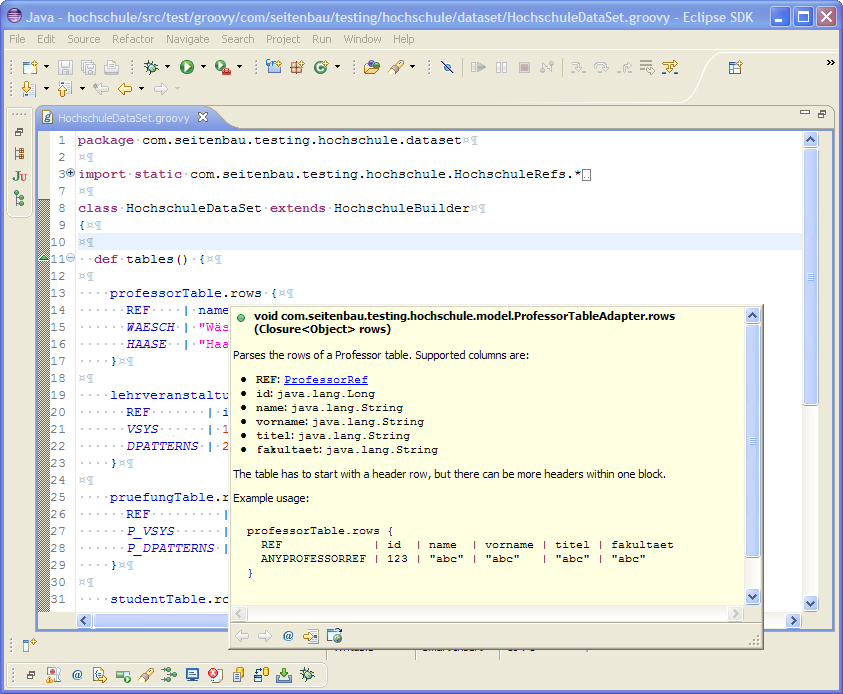
\includegraphics[width=0.9\textwidth]{images/realisierung/javadoc_tooltip.png}
  \caption{Beispiel JavaDoc-Tooltip}\label{img:javadoc_tooltip}
\end{figure}

  \section{Verhalten bei Fehlern in den Tabellendefinitionen}
  \label{sec:ralisierungdsl:verhaltenfehler}
  
  Selbst eine �bersichtliche Darstellung von Tabellendaten sch�tzt nicht vor Fehleingaben. Viele Fehler lassen sich mit
  Hilfe statischer Analysen erkennen. So werden ung�ltige Tabellen- und Spaltennamen vom Compiler entdeckt.

  Fehler in der eigentlichen Tabellenstruktur, z.B. eine abweichende Anzahl von Spalten, kann der Standard-Compiler
  nicht erkennen, genauso wie ung�ltige Werte bzw. ung�ltige Typen. Solche Fehler werden in der gegenw�rtigen
  Implementierung erst zur Laufzeit erkannt und f�hren zum Scheitern der Tests. Dazu wirft der Tabellen-Parser eine
  Exception der Klasse \texttt{TableParserException}. Wenn ein falscher Typ verwendet wird, k�nnte die Meldung
  der Exception so aussehen: \textit{Cannot set value <5> of type java.lang.Integer, expected class java.lang.String
  in [TableRowModel: <JobsRef> | 5 | "Creating software"]}
  
  Um die Lokalisation der fehlerhaften Stelle zu erleichtern, wird der Stack-Trace der geworfenen Exception angepasst.
  Die Arbeitsweise Tabellen-Parsers macht dies notwendig: Der Parser arbeitet zeilenweise,
  d.h. er liest immer eine Zeile vollst�ndig ein und interpretiert die Daten erst im Anschluss - wenn die
  Ausf�hrung der Zeile abgeschlossen ist. Kommt es zu einem Fehler, befindet sich das Programm aber nicht mehr
  in der Zeile, die f�r den Fehler verantwortlich ist. Deshalb wird beim Parsen bei jedem Tabellen-Element der Stack-Trace
  analysiert und das Stack-Trace-Element bestimmt, das zu der Tabellenzeile geh�rt. Sollte es beim Setzen
  der Werte einen Fehler geben, wird dieses Element als erstes Element des Stack-Traces hinzugef�gt.
	Der Vorteil der Stack-Trace-Manipulation ist, dass im Falle eines Fehlers der Tester schnell �ber den Stack-Trace
	die richtige Stelle im Code finden kann.
	

  \section{Nicht umgesetzt}
  \label{sec:ralisierungdsl:nichtumgesetzt}
  
  Der folgende Abschnitt soll einen kurzen �berblick �ber nicht umgesetzte Funktionen geben. Au�erdem wird begr�ndet,
  warum diese Funktionen nicht in \textit{STU} implementiert ist.

    \subsection{Zusammengesetzte Schl�ssel}
    Zusammengesetzte Schl�ssel werden in \textit{STU} nicht direkt unterst�tzt und m�ssen nach wie vor komplett
		manuell realisiert werden. Dazu muss f�r jeden Teilschl�ssel eine
    Spalte im Datenbank-Modell angelegt werden. Sofern zum Zugriff auf Tabellenzeilen die Referenz-Typen
    verwendet werden, stellt das kein gro�es Problem dar. Sollte die Zeile in Abh�ngigkeit ihres
    Schl�ssels dynamisch gesucht werden, kann auf die neue \texttt{find}-Methode zur�ckgegriffen werden.

    \subsection{Unterst�tzung f�r weitere Beziehungstypen}
    Folgende Beziehungstypen m�ssen manuell umgesetzt werden.
    
    \begin{itemize}
      \item \textbf{Reflexive Beziehungen}
        Eine reflexive Beziehung kann in \textit{STU} nur manuell ausgedr�ckt werden. Die Definition einer
        einfachen Tabelle f�r einen Baum, der aus einzelnen Knoten besteht, k�nnte wie folgt aussehen
        (siehe Listing \ref{listing:reflexiv:manuell}). Ein Knoten-Element kennt den zugeh�rigen Eltern-Knoten
        (Zeile 5). Eine Referenz auf die Tabelle ist an dieser Stelle nicht m�glich, die Relation muss
        manuell ohne besondere Tool-Unterst�tzung durch \textit{STU} realisiert werden.
      
        \begin{lstlisting}[caption=Reflexive Beziehungen manuell, label=listing:reflexiv:manuell]
Table knoten = table("knoten")
    .column("id", DataType.BIGINT)
      .defaultIdentifier()
    .column("name", DataType.VARCHAR)
    .column("parent", DataType.BIGINT)
  .build();
        \end{lstlisting} 
        
        Die Konsequenz ist, dass die Beziehungen nicht typsicher �ber die Referenz-Klasse modelliert werden
        k�nnen, sondern die Prim�r- und Fremdschl�ssel manuell im DataSet gepflegt werden m�ssen.
        
        Ein anderer Ansatz stellt das Refaktorisieren der Datenbank und der beteiligten Systeme dar. Dies ist
        leider nicht immer m�glich. Die Refaktorisierung sieht eine assoziative Tabelle f�r die Modellierung
        der Beziehung vor (siehe Listing \ref{listing:reflexiv:assoc}).
        
        \begin{lstlisting}[caption=Reflexive Beziehungen mit Hilfe assoziativer Tabelle, label=listing:reflexiv:assoc]
Table knoten = table("knoten")
    .column("id", DataType.BIGINT)
      .defaultIdentifier()
    .column("name", DataType.VARCHAR)
  .build();

associativeTable("parents")
    .column("parent", DataType.BIGINT)
      .reference
        .foreign(knoten)
    .column("child", DataType.BIGINT)
      .reference
        .foreign(knoten)
  .build();
        \end{lstlisting} 

      \item \textbf{Zirkul�re Beziehungen}
				Reflexive Beziehungen stellen eine besondere Form von zirkul�ren Beziehungen dar. Die Probleme sind
				relativ �hnlich. Als kleines Modell dient eine Veranstaltungsplanung, bei der es Organisatoren
				und Teilnehmer geben kann. Eine Veranstaltung wird von einer Person organisiert, eine Person
				kann an einer Veranstaltung teilnehmen. Listing \ref{listing:zirkulaer:manuell} zeigt eine
				Realisierung dieses Modells.

        \begin{lstlisting}[caption=Zirkul�re Beziehungen manuell, label=listing:zirkulaer:manuell]
Table event = table("event")
    .column("id", DataType.BIGINT)
      .defaultIdentifier()
    .column("name", DataType.VARCHAR)
    .column("organizer", DataType.BIGINT)  // a person
  .build();

Table person = table("person")
    .column("id", DataType.BIGINT)
      .defaultIdentifier()
    .column("name", DataType.VARCHAR)
    .column("participates", DataType.BIGINT)
      .reference
        .foreign(event)
  .build();
        \end{lstlisting} 
      
			  Dasselbe Modell l�sst sich -- aus Sicht von \textit{STU} -- etwas typsicherer umsetzen.
				F�r die Teilnahme wird eine assoziative Tabelle verwendet. Dar�ber hinaus kann hier auch
				eine Person an mehreren Veranstaltungen teilnehmen. Listing \ref{listing:zirkulaer:assoc}
				zeigt die Realisierung einer zirkul�ren Beziehung mit Hilfe einer assoziativen Tabelle.
      
        \begin{lstlisting}[caption=Zirkul�re Beziehungen mit assoziativer Tabelle, label=listing:zirkulaer:assoc]
Table person = table("person")
    .column("id", DataType.BIGINT)
      .defaultIdentifier()
    .column("name", DataType.VARCHAR)
  .build();

Table event = table("event")
    .column("id", DataType.BIGINT)
      .defaultIdentifier()
    .column("name", DataType.VARCHAR)
    .column("organizer", DataType.BIGINT)
  .build();

associativeTable("parcipations")
    .column("event", DataType.BIGINT)
      .reference
        .foreign(event)
    .column("participant", DataType.BIGINT)
      .reference
        .foreign(person)
  .build();
        \end{lstlisting} 
      
      \item \textbf{Tern�re und andere h�hergradige Beziehungen}
			  \textit{STU} sieht keine spezielle Unterst�tzung f�r tern�re oder andere h�hergradige Beziehungen vor.
				Es bietet sich an, solche Beziehungen �ber eine zus�tzliche Tabelle zu realisieren (siehe Listing
				\ref{listing:hoehergradig}, vergleichbar mit assoziativen Beziehungen f�r die Modellierung von
				n:m-Beziehungen.

        \begin{lstlisting}[caption=H�hergradige Beziehungen mit zus�tzlicher Tabelle, label=listing:hoehergradig]
Table student = table("student")
    .column("id", DataType.BIGINT)
      .defaultIdentifier()
    .column("name", DataType.VARCHAR)
  .build();

Table professor = table("professor")
    .column("id", DataType.BIGINT)
      .defaultIdentifier()
    .column("name", DataType.VARCHAR)
  .build();

Table pruefung = table("pruefung")
    .column("id", DataType.BIGINT)
      .defaultIdentifier()
    .column("name", DataType.VARCHAR)
  .build();

table("relation")
    .column("student_id", DataType.BIGINT)
      .reference
        .foreign(student)
    .column("professor_id", DataType.BIGINT)
      .reference
        .foreign(professor)
    .column("pruefung_id", DataType.BIGINT)
      .reference
        .foreign(pruefung)
  .build();
        \end{lstlisting} 
			
    \end{itemize}
  
    \subsection{Komfortfunktionen}
    
    Die Realisierung k�nnte an manchen Stellen dem Test-Ingenieur mehr manuelle Arbeit abnehmen. So wird darauf verzichtet,
    beim L�schen einer Zeile aus einer Tabelle auch alle beteiligten Beziehungen zu entfernen. Listing \ref{listing:deleteexample}
    zeigt, wie ein Professor aus der Professoren-Tabelle entfernt wird. Die erste Zeile entfernt keine Eintr�ge in 
    anderen Tabellen wie z.B. der Beaufsichtigt-Tabelle. Folglich m�ssen die Relationen (mehr oder weniger) manuell
    aus anderen Tabellen entfernt werden.

    \begin{lstlisting}[caption=L�schen von Zeilen, label=listing:deleteexample]
dataSet.professorTable.deleteRow(HAASE);
dataSet.beaufsichtigtTable.deleteAllAssociations(HAASE);
    \end{lstlisting} 
  
    Diese Entscheidung hat unterschiedliche Gr�nde:
    \begin{itemize}
      \item \textbf{Einsatzgebiet}: Die Bibliothek soll Unit-Tests in Verbindung mit Datenbanken vereinfachen. Es handelt sich
        hier nicht um ein API, das in einer Anwendung ausgeliefert wird. W�hrend es in einem API f�r produktive Anwendungen
        durchaus sinnvoll sein kann, dass das System beim L�schen von Entit�ten gewisse Aufgaben automatisch erledigt,
        ist so ein Verhalten innerhalb einer Test-Bibliothek zweifelhaft. Explizites L�schen von Zeilen auf allen beteiligten
        Tabellen verbessert die Ausdrucksst�rke des Tests.
        
      \item \textbf{Code-Qualit�t}: Eine Funktion (bzw. Methode) sollte genau eine Aufgabe erledigen. Wenn
        \texttt{deleteRow} zus�tzlich beteiligte Relationen aufl�st, erledigt diese Funktion mehr als nur eine Aufgabe 
        \cite[65f]{CLEAN_CODE}. Au�erdem w�rde es sich um einen unerwarteten Nebeneffekt handeln \cite[75f]{CLEAN_CODE}.
      
      \item \textbf{Klarheit}: Es ist nicht eindeutig, wie beim Entfernen von Zeilen vorgegangen werden soll, wenn sie
        Teil einer Relation sind. Bei einer n:m-Relation k�nnte sich die Regel ableiten lassen, dass beim L�schen einer
        Zeile auch alle assoziierten n:m-Relationen entfernt werden k�nnen. Aber was ist bei einer 1:n-Relation? Wenn
        ein Professor entfernt wird, was soll mit Lehrveranstaltungen passieren, die ihm zugeordnet sind?
    \end{itemize}

	\chapter{Generieren von Testdaten}
\label{chap:generieren}

Es gibt verschiedene Ans�tze zur Generierung von Testdaten f�r Datenbank-basierte Anwendungen:
\begin{enumerate}
  \item \textbf{Modell-basierte, Abfrage-unabh�ngige Generierung}:
  	Anhand eines Datenbank-Modells werden Entit�ten mit Zufallswerten f�r die Attribute (Spalten) erzeugt. Es gibt
  	einige kommerzielle Werkzeuge aber auch frei nutzbare Internet-Seiten f�r die Generierung. 
  
  \item \textbf{Modell-basierte, Abfrage-basierte Generierung}:
  	Ausgehend von konkreten Abfragen (z.B. in SQL) werden f�r die Abfrage passende Daten erzeugt. Binnig beschreibt in
  	\cite{DBLP:conf:icde:BinnigKL07} einen Ansatz, bei dem SQL-Abfragen als Grundlage f�r die Daten-Generierung verwendet
		werden. Mit AGENDA wird in \cite{Chays04anagenda} ein Toolset vorgestellt, das neben dem Datenbank-Schema den
		Anwendungsquellcode betrachtet.
  
  \item \textbf{Anonymisierung realer Daten}:
  	Bei diesem Ansatz findet keine echte Generierung statt. Stattdessen werden Daten einer realen Anwendung 
  	anonymisiert und f�r Tests verwendet.
  
\end{enumerate}

F�r die Generierung eines Standard Fixtures scheint nur die erste Variante sinnvoll zu sein: Es liegt bereits
ein Modell vor und die generierten Daten sollen idealerweise f�r alle Tests verwendet werden k�nnen.
Konkrete Anfragen als Grundlage f�r die Generierung sind nicht sinnvoll. Einerseits k�nnen sie
vom SUT verborgen werden k�nnen, andererseits eigenen sie eher f�r Fixtures, die f�r einen einzelnen Unit-Test
geeignet sind. Die Anonymisierung realer Daten stellt keine Daten-Generierung im eigentlichen Sinn dar und
setzt bestehende Daten voraus.

Eine Auswahl existierender Modell-basierter, Abfrage-unabh�ngiger Datengeneratoren wird im folgenden Abschnitt
auf die Anwendbarkeit hin untersucht.


\section{Betrachtung existierender Werkzeuge}
\label{sec:generieren:analyse}

Es gibt bereits eine Reihe von Werkzeugen zur Generierung von Zufallsdaten f�r Datenbanken. In wie weit sich diese
f�r die Aufgabenstellung nutzen lassen, soll im folgenden kurz analysiert werden.

  \subsection{Kommerzielle Werkzeuge}
	\label{sec:generieren:analyse:kommerziellewerkzeuge}
	Zu den betrachteten kommerziellen Anwendungen z�hlen:

	\begin{itemize}
		\item \textbf{Datanamic Data Generator MultiDB}: \\
			\url{http://www.datanamic.com/datagenerator/}
		\item \textbf{DTM Data Generator}: \\
			\url{http://www.sqledit.com/dg/}
		\item \textbf{forSQL Data Generator}: \\
			\url{http://www.forsql.com/}
		\item \textbf{Red Gate SQL Data Generator}: \\
			\url{http://www.red-gate.com/products/sql-development/sql-data-generator/}
	\end{itemize}

	Insgesamt sind die M�glichkeiten der Anwendungen relativ �hnlich. Die gr��ten Unterschiede aus Nutzer-Sicht liegen in der
	Bedienung. Die Werkzeuge arbeiten zufallsbasiert aber deterministisch, d.h. sie erzeugen bei gleichem Modell die gleichen
	Daten. Das sogenannte \textit{Seed}, mit dem der Zufallszahlengenerator f�r eine einzelne Spalte initialisiert wird, l�sst
	sich z.B. beim Red Gate SQL Data Generator komfortabel festlegen.

	Die Werkzeuge sind vor allem f�r die Generierung von gro�en Datenmengen (Massen-Daten) vorgesehen. Dies zeigt sich auch darin,
	dass sie Beziehungen auch nur zuf�llig modellieren. �ber eine entsprechend gro�e Menge an Testdaten soll dann auch jeder
	notwendige Fall abgedeckt sein. Die Menge der zu erzeugenden Testdaten l�sst sich f�r jede einzeln Tabelle konfigurieren.
	Eigene Vorschl�ge, wie viele Daten generiert werden sollten, machen die Werkzeuge nicht.

  \subsection{Andere Ans�tze}
	\label{sec:generieren:analyse:andereansaetze}
	
	In \cite{Houkjaer:2006:SRD:1182635.1164254} wird ein Algorithmus zur Generierung von Test-Daten vorgestellt, der
	das Datenbank-Modell als Graphen betrachtet. Tabellen stellen Knoten und ihre Beziehungen stellen gerichtete
	Kanten dar. Die Anzahl der generierten Entit�ten wird �ber Verh�ltnisse vom Tester konfiguriert. Auch dieser Algorithmus
	ist eher f�r die Erzeugung von Massen-Daten geeignet.


	\subsection{Fazit}
	Die von dem zu entwickelnden Generator erzeugten Testdaten sollen allerdings �berschaubar und wartbar sein. Dies steht
	in Widerspruch mit einer Massen-Daten-Generierung, wie sie die kommerziellen Werkzeuge bieten. Zum selben Schluss kommt
	Raza in \cite[126]{CREATINGDATASETS}. Massen-Daten eignen sich eher f�r Stabilit�ts-, Performance- und Regressionstests.
		
  Keines der kommerziellen Werkzeuge ist in der Lage, die Anzahl der zu generierenden Entit�ten selbst zu bestimmen. Auch
	der Algorithmus aus \cite{Houkjaer:2006:SRD:1182635.1164254} ist dazu nicht in der Lage.
	
	Aus diesem Grund soll ein Algorithmus entwickelt werden, der Beziehungen nicht nur zuf�llig generiert, sondern m�glichst
	alle Grenzf�lle erzeugt.  �quivalenzklassenbildung und Grenzwertanalyse sind ein bew�hrtes Vorgehen, um die Menge von
	Test-Daten zu reduzieren. 
	


\section{Generierung von Beziehungen}

Der zu entwickelnde Algorithmus �bernimmt das Konzept der �quivalenzklassenbildung und Grenzwertanalyse, um m�glichst
alle notwendigen Beziehungskombinationen zwischen zwei Entit�tstypen zu modellieren. Die Menge der zu generierenden
Entit�ten soll dabei m�glichst gering gehalten werden.

Unterschiedliche Beziehungstypen stellen unterschiedliche Anforderungen an den Daten-Generator. Bin�re Beziehungstypen
lassen sich in die drei Hauptkategorien 1:1, 1:n und n:m einordnen. Die folgenden Abbildungen stellen die zu generierenden
Entit�ten der beiden Entit�tstypen A und B dar. Eine Entit�t wird von einem kleinen Kreis repr�sentiert, ihr 
Entit�tstyp �ber die Spalte festgelegt. Eine Beziehung zwischen zwei Entit�ten wird �ber eine Verbindungsgerade
beschrieben. Grunds�tzlich k�nnen die beiden Typen A und B auch den selben Typen darstellen.

Ganz allgemein lassen sich alle bin�ren Beziehungen als n..N:m..M-Beziehung ansehen. n und m stellen jeweils
untere Grenzen darf, N und M die oberen. Die grundlegende Generierungsstrategie sieht die Generierung der folgenden
vier Kombinationen vor:
\begin{itemize}
  \item n:m
  \item n:M
  \item N:m
  \item N:M
\end{itemize}
Verschiedene F�lle k�nnen redundant sein, falls untere und obere Grenze identisch sind. Auf die Generierung dieser
redundanten Beziehungen kann verzichtet werden.

Die Abbildungen stellen dar, welche Entit�ten und Beziehungen \textit{mindestens} generiert werden sollten, um
die von den Grenzen der Multiplizit�ten bestimmten �quivalenzklassen abzudecken.

  \subsection{Kategorie der 1:1-Beziehungen}
  
  Unter die Kategorie 1:1-Beziehung fallen alle Beziehungstypen, bei denen eine oder keine Entit�t mit genau einer oder
  keiner Entit�t in Beziehung stehen kann.
  
  	\subsubsection{1..1:1..1}
		\label{sec:generieren:categories:11to11}
  	
  	Eine Entit�t des Typs A steht mit genau einer Entit�t des Typs B in Beziehung. Die Anzahl der generierten Entit�ten
  	muss �bereinstimmen, es muss mindestens eine Entit�t pro Typ erzeugt werden (siehe Abbildung \ref{img:generierung:11to11}).
  	
  	\begin{figure}[htbp]
  	  \centering
  	   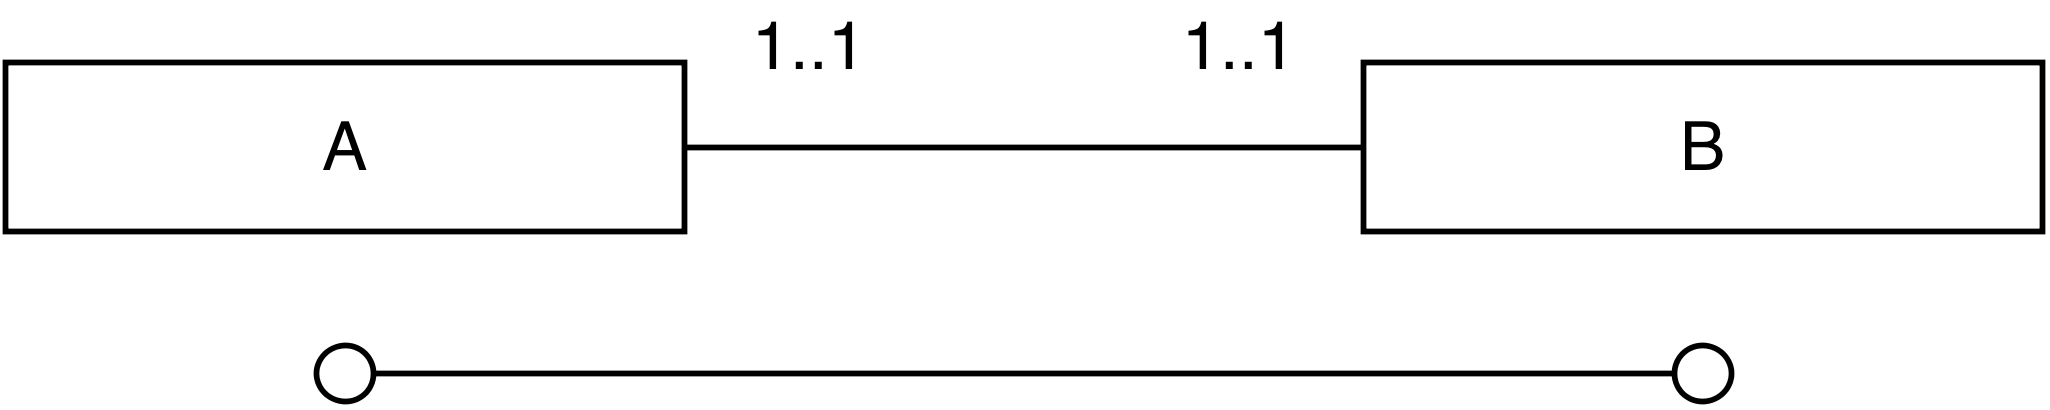
\includegraphics[width=0.55\textwidth]{images/generierung/1-1-to-1-1.png}
  	  \caption{Beziehungen nach dem Schema 1..1:1..1}\label{img:generierung:11to11}
  	\end{figure}

  	
  	\subsubsection{0..1:1..1}
		\label{sec:generieren:categories:01to11}
  	
  	Im Gegensatz zu demr vorherigen Beziehungstyp muss bei dieser eine Entit�t nicht zwingend in Beziehung mit einer anderen stehen.
  	Abbildung \ref{img:generierung:01to11} zeigt die zu generierenden Entit�ten der Typen A und B, wobei jede Entit�t von A
  	mit einer Entit�t von B in Beziehung stehen muss, eine Entit�t von B jedoch nicht zwingend mit einer Entit�t von A.
  	Daraus folgt, dass es von B mindestens eine Entit�t mehr geben muss als von A.

  	\begin{figure}[htbp]
  	  \centering
  	   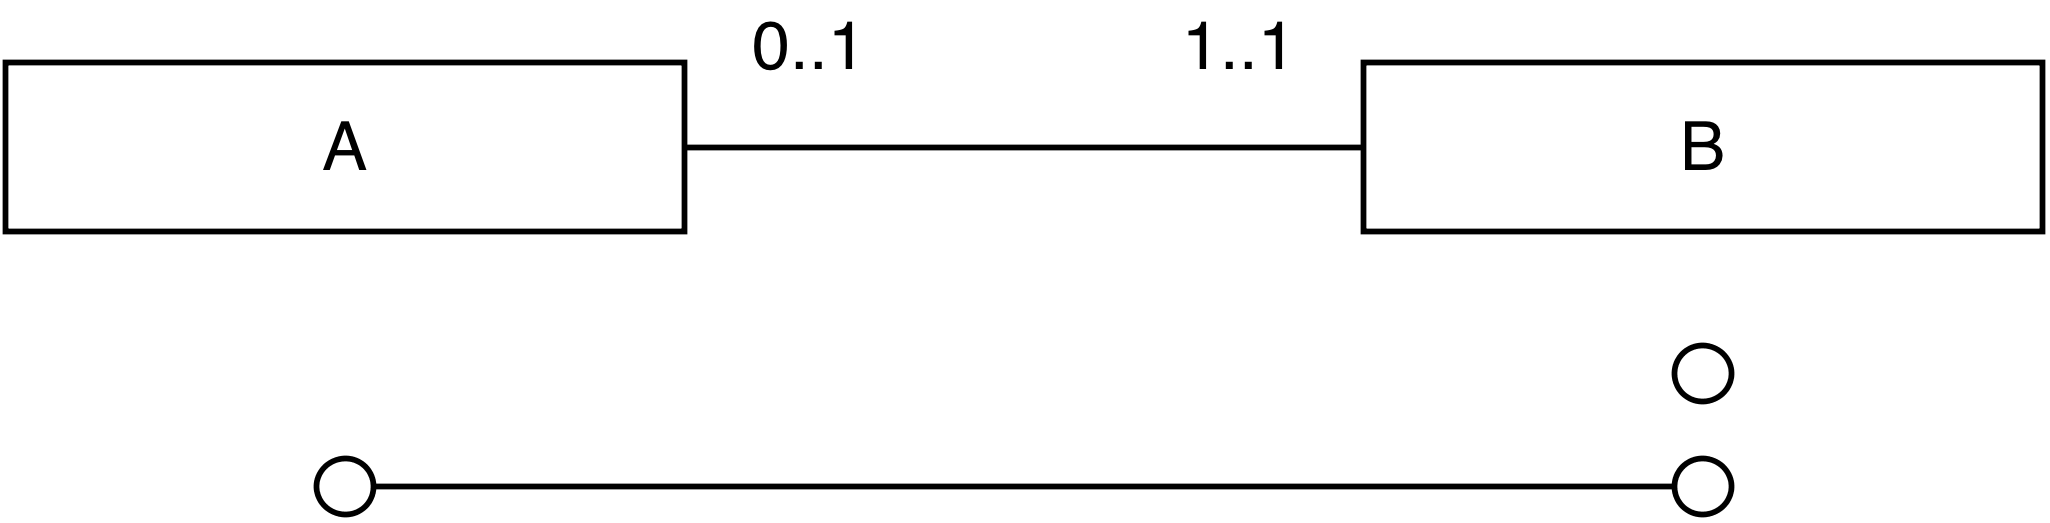
\includegraphics[width=0.55\textwidth]{images/generierung/0-1-to-1-1.png}
  	  \caption{Beziehungen nach dem Schema 0..1:1..1}\label{img:generierung:01to11}
  	\end{figure}

  	Der Generator muss mindestens zwei Entit�ten des Typs B erzeugen, und eine des Typs A, um sicherzustellen, dass alle
  	F�lle f�r diese Beziehung abgedeckt sind. 
		
		Die Beziehung 1..1:0..1 ist symmetrisch zu dieser.
  	

  	\subsubsection{0..1:0..1}
		\label{sec:generieren:categories:01to01}
  	
  	Wenn f�r beide Entit�tstypen die Beziehung optional ist, muss der Generator jeweils mindestens 2 Entit�ten erzeugen. Jeweils
  	eine Entit�t ohne Beziehung und jeweils eine Entit�t mit einer Beziehung (siehe Abbildung \ref{img:generierung:01to01}).

  	\begin{figure}[htbp]
  	  \centering
  	   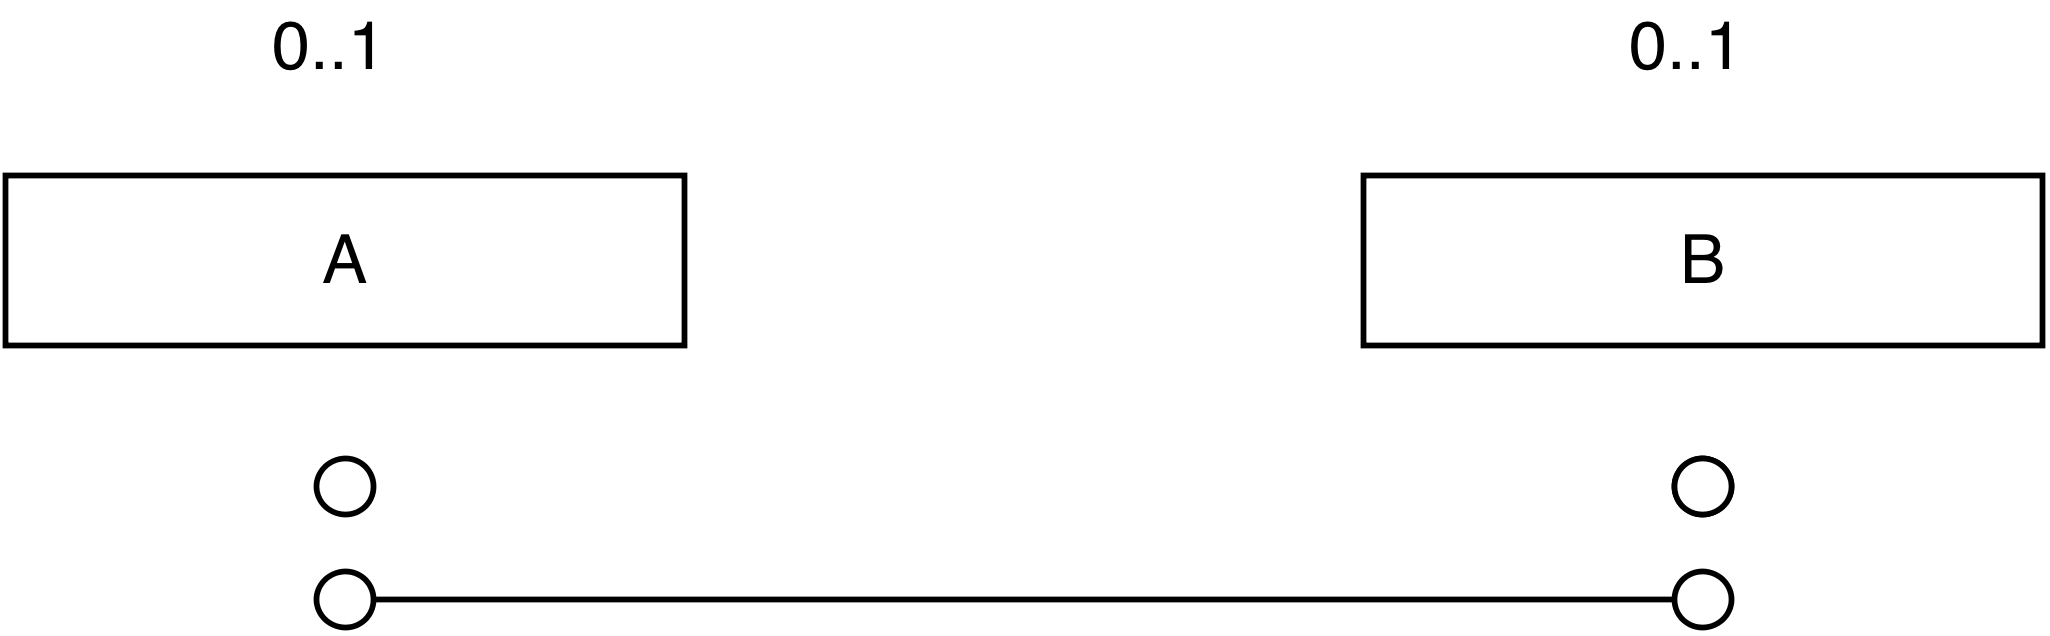
\includegraphics[width=0.55\textwidth]{images/generierung/0-1-to-0-1.png}
  	  \caption{Beziehungen nach dem Schema 0..1:0..1}\label{img:generierung:01to01}
  	\end{figure}

  \subsection{Kategorie der 1:n-Beziehungen}
  
  Eine Entit�t steht in Beziehung mit keiner oder mehreren anderen Entit�ten. Dabei kann die Anzahl begrenzt sein (konkreter
  Wert f�r n) oder unbegrenzt. Der Generator kann nur eine begrenzte Anzahl von Entit�ten erzeugen, die Grenze sollte
  konfigurierbar sein.
  
  	\subsubsection{1..1:1..n}
		\label{sec:generieren:categories:11to1n}
  	
  	Die einfachste Form der 1:n-Beziehungen. Eine Entit�t des Typs A ist in einer Beziehung mit einer oder mehreren Entit�ten
  	des Typs B. Eine Entit�t des Typs B ist mit genau einer Entit�t des Typs A in Beziehung. Die zu generierenden Entit�ten 
		sind in Abbildung \ref{img:generierung:11to1n} dargestellt.

  	\begin{figure}[htbp]
  	  \centering
  	   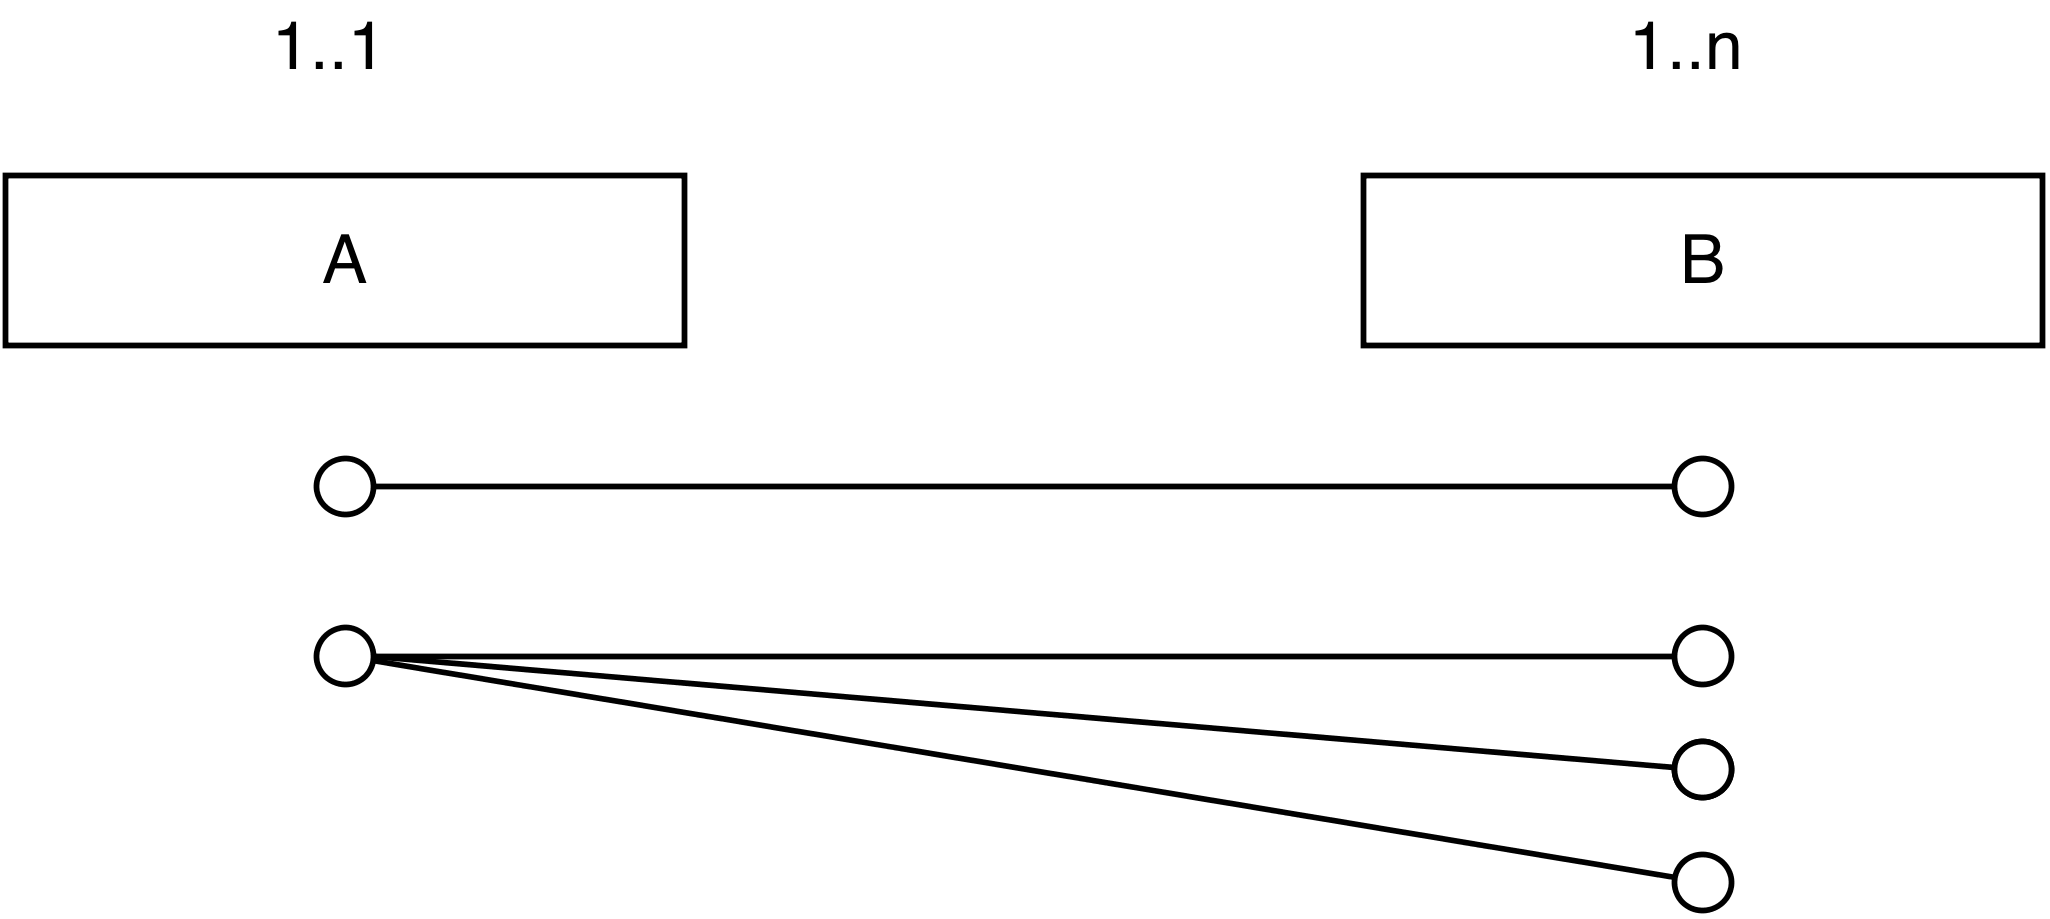
\includegraphics[width=0.55\textwidth]{images/generierung/1-1-to-1-n.png}
  	  \caption{Beziehungen nach dem Schema 1..1:1..n}\label{img:generierung:11to1n}
  	\end{figure}

  	\subsubsection{0..1:1..n}
		\label{sec:generieren:categories:01to1n}
  	
  	Eine Entit�t des Typs A steht in Beziehung mit einer oder mehreren Entit�ten des Typs B. Eine Entit�t des Typs B steht
  	entweder mit genau einer oder mit keiner Entit�t des Typs A in Beziehung. Abbildung \ref{img:generierung:01to1n} stellt
		die zu generierenden Entit�ten dar. 

  	\begin{figure}[htbp]
  	  \centering
  	   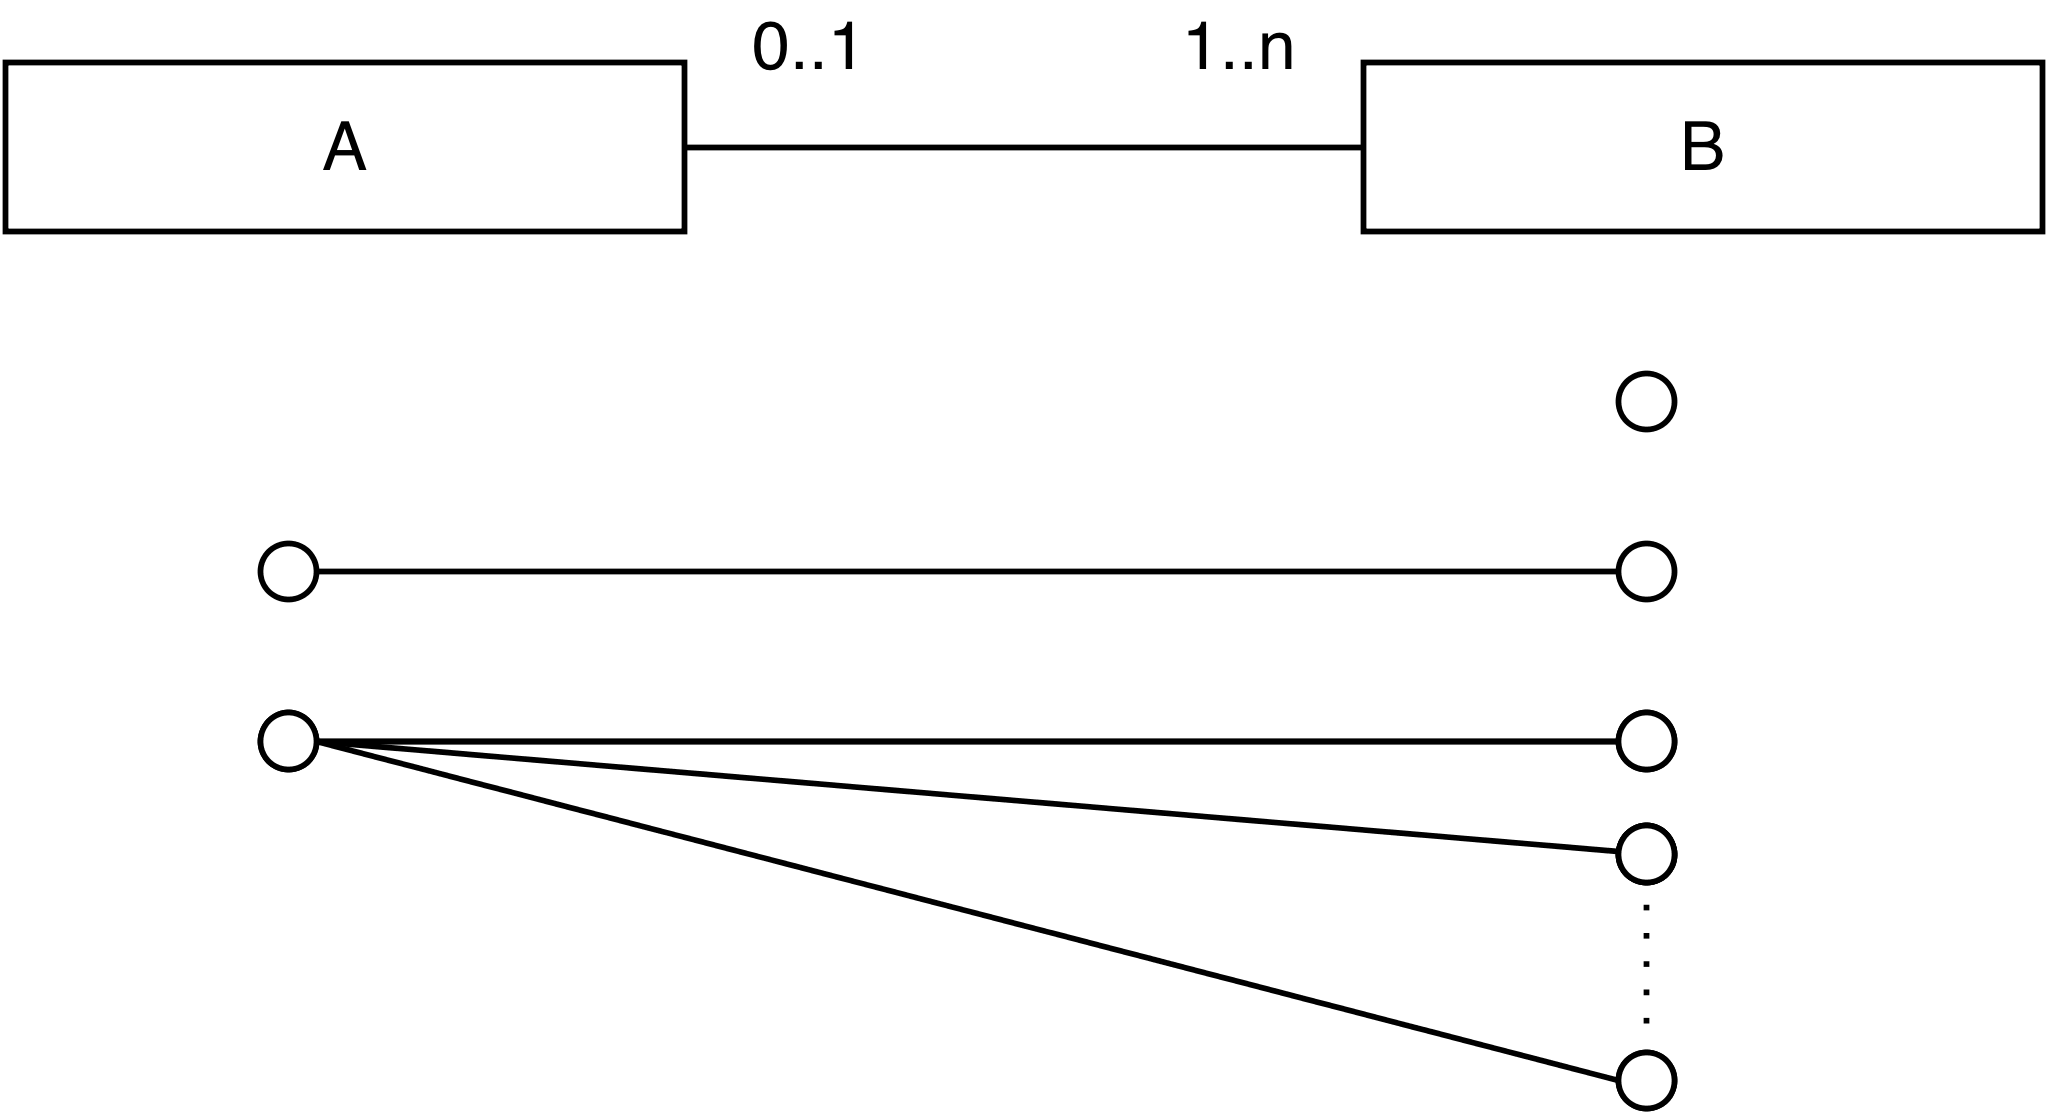
\includegraphics[width=0.55\textwidth]{images/generierung/0-1-to-1-n.png}
  	  \caption{Beziehungen nach dem Schema 0..1:1..n}\label{img:generierung:01to1n}
  	\end{figure}
  	
  	\subsubsection{1..1:0..n}
		\label{sec:generieren:categories:11to0n}
  	
  	Eine Entit�t des Typs A steht in Beziehung mit keiner, einer oder mehreren Entit�ten des Typs B. Eine Entit�t des Typs B
  	muss mit genau einer Entit�t des Typs A in Beziehung stehen. 

  	\begin{figure}[htbp]
  	  \centering
  	   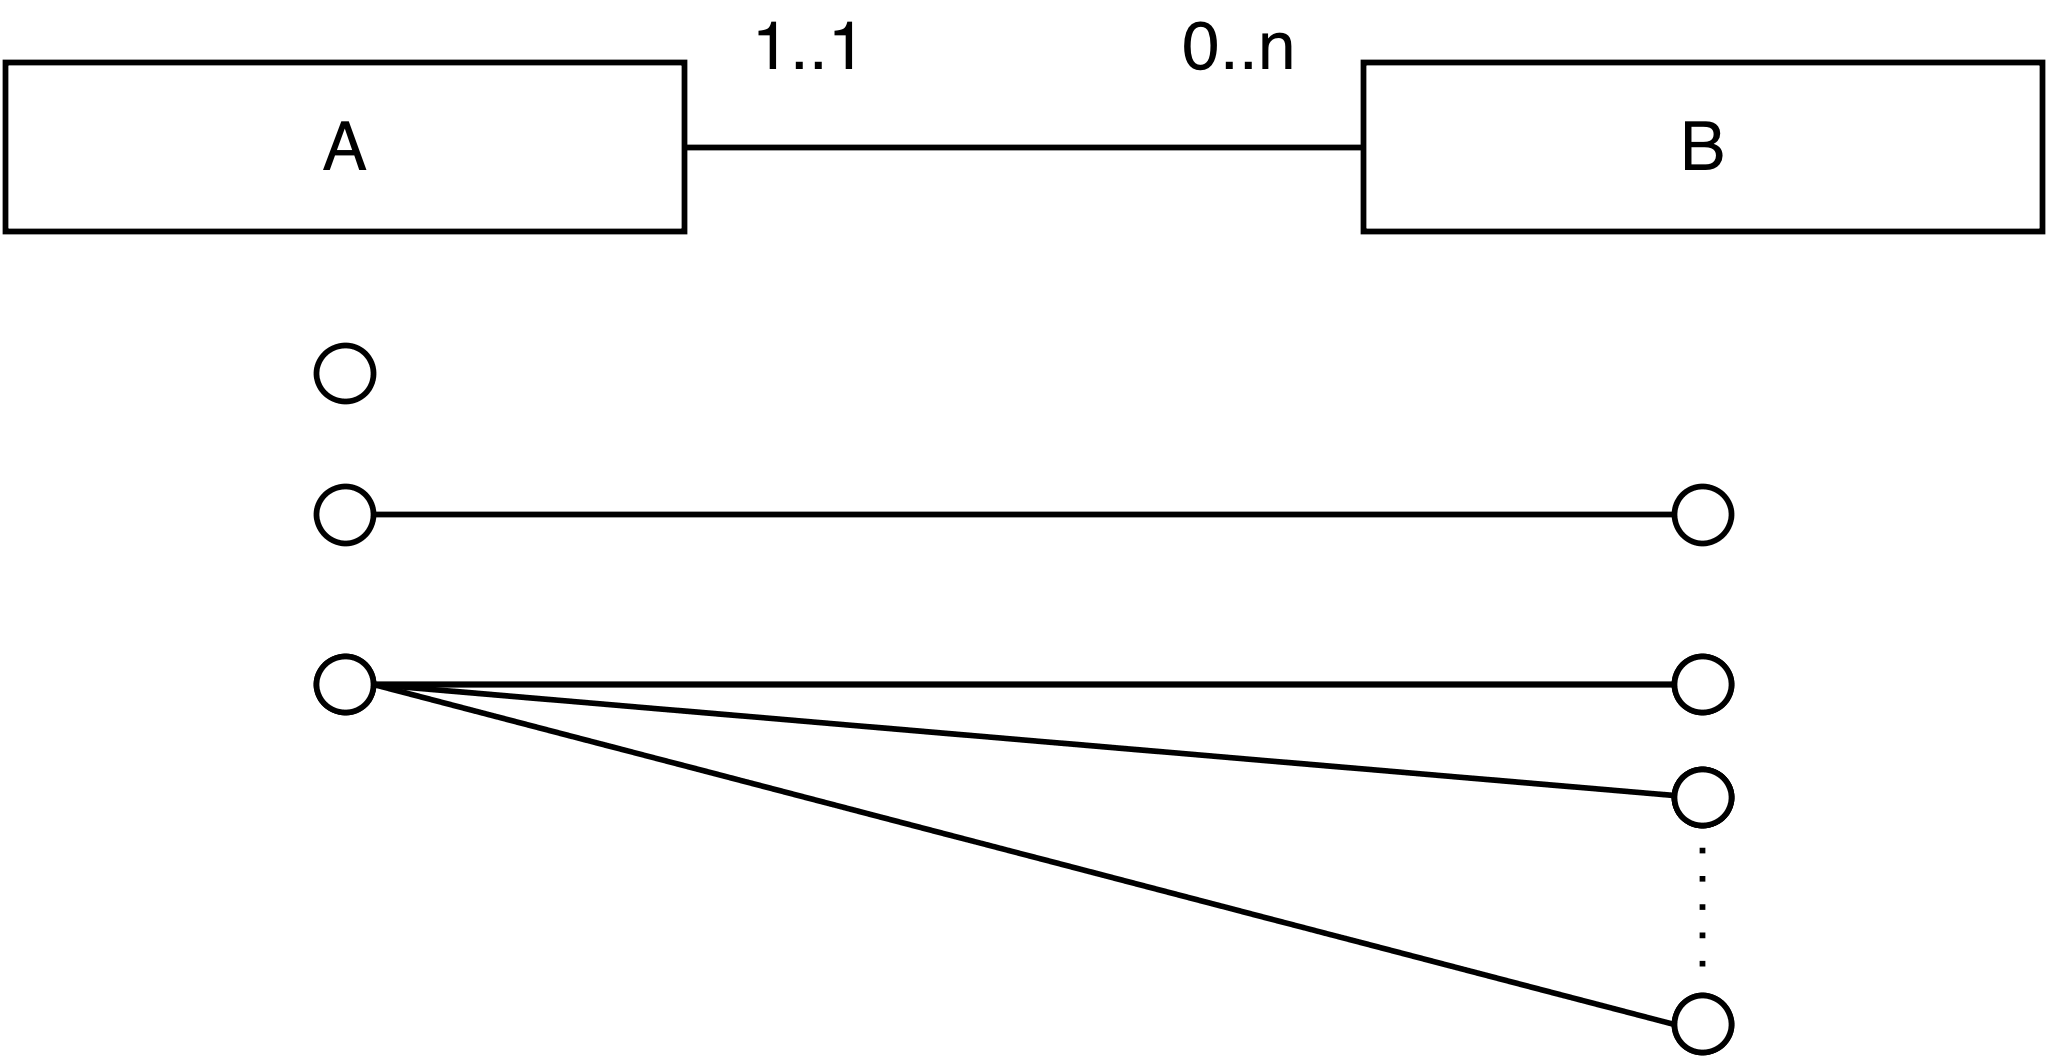
\includegraphics[width=0.55\textwidth]{images/generierung/1-1-to-0-n.png}
  	  \caption{Beziehungen nach dem Schema 1..1:0..n}\label{img:generierung:11to0n}
  	\end{figure}



  	\subsubsection{0..1:0..n}
		\label{sec:generieren:categories:01to0n}
		
		Eine Entit�t des Typs A steht mit keiner, einer oder mehreren Entit�ten des Typs B in Beziehung. Eine Entit�t des Typs B
		kann mit keiner oder genau einer Entit�t des Typs A in Beziehung stehen.

  	\begin{figure}[htbp]
  	  \centering
  	   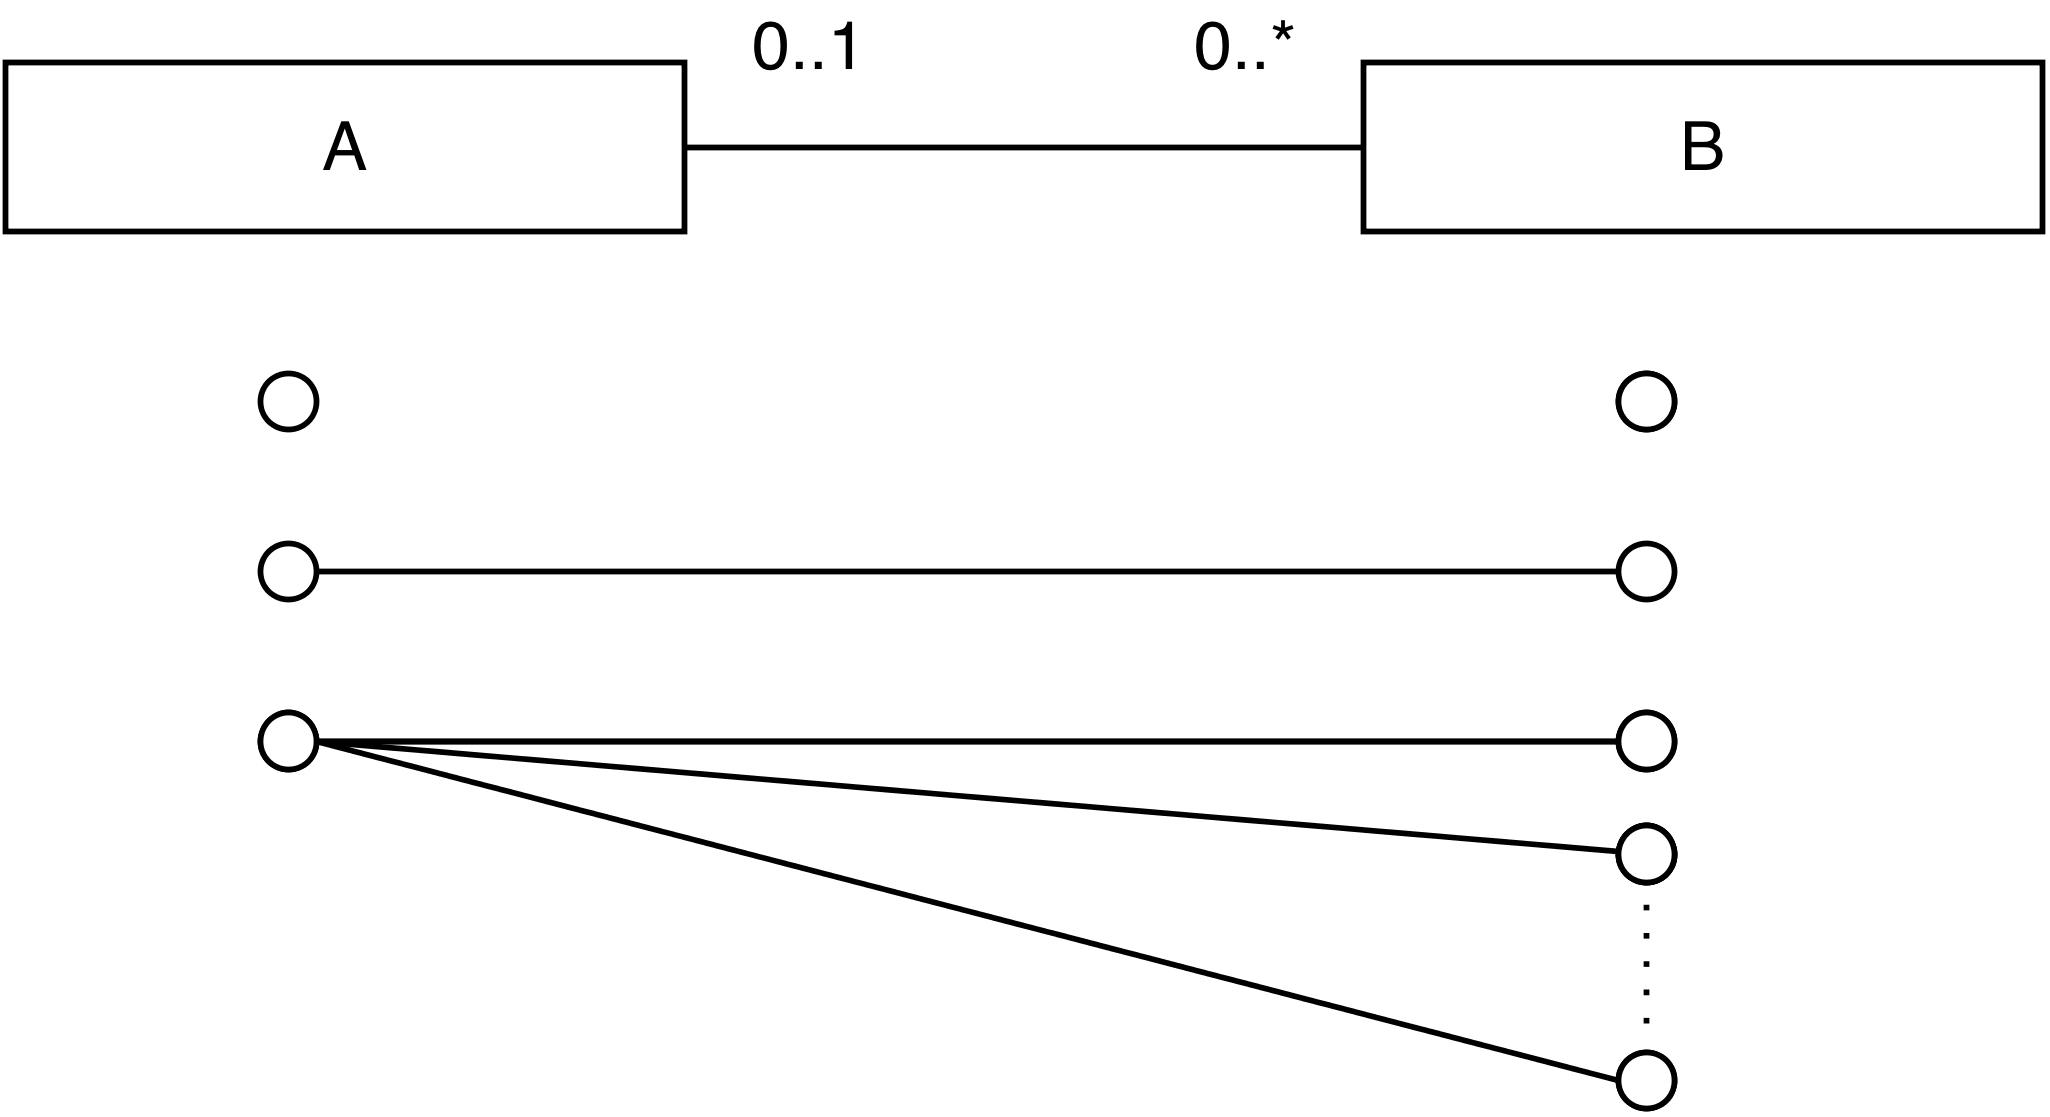
\includegraphics[width=0.55\textwidth]{images/generierung/0-1-to-0-n.png}
  	  \caption{Beziehungen nach dem Schema 0..1:0..n}\label{img:generierung:01to0n}
  	\end{figure}

  \subsection{Kategorie der n:m-Beziehungen}
	\label{sec:generieren:beziehungen:nm}
		
	Die allgemeinste Form einer Beziehung zwischen zwei Eintit�tstypen stellt eine n..N:m..M-Beziehung dar. Dabei handelt es
	sich bei n und m jeweils um untere und bei N und M jeweils um obere Schranken. Untere und obere Schranken k�nnen
	identisch sein.
	
	Jede der in diesem Abschnitt beschriebenen Beziehungsformen stellen Spezialf�lle von n:m-Beziehungen dar, bei denen
	eine oder beide oberen Grenzen 1 sind. Sind beide obere Grenzen gr��er als 1, dann wird eine solche Beziehung
	�blicherweise �ber assoziative Tabellen realisiert.
	
	Sollte eine der unteren Grenzen 0 sein, wird sie als 0..1 interpretiert. D.h es wird eine entsprechende Entit�t ohne
	Beziehung erzeugt, aber auch eine einzelne Entit�t, die in Beziehung mit anderen Entit�ten steht 
	(siehe dazu Abbildungen \ref{img:generierung:1to01} und \ref{img:generierung:3to01}).
	
	Um die unterschiedlichen Kombinationen aus n, N, m und M in den Grafiken zu verdeutlichen, wird als Beziehung eine
	1..3:0..4-Beziehung verwendet.
	
		\subsubsection{1. Fall (n:m): 1:0..1}
		
		
		Im ersten Fall werden beide unteren Grenzen betrachtet. Da eine der Grenzen 0 ist, wird eine Entit�t ohne Beziehung
		generiert. Abbildung \ref{img:generierung:1to01} visualisiert die zu erzeugenden Entit�ten f�r die Kombination n:m.
		
	  \begin{figure}[htbp]
  	  \centering
  	   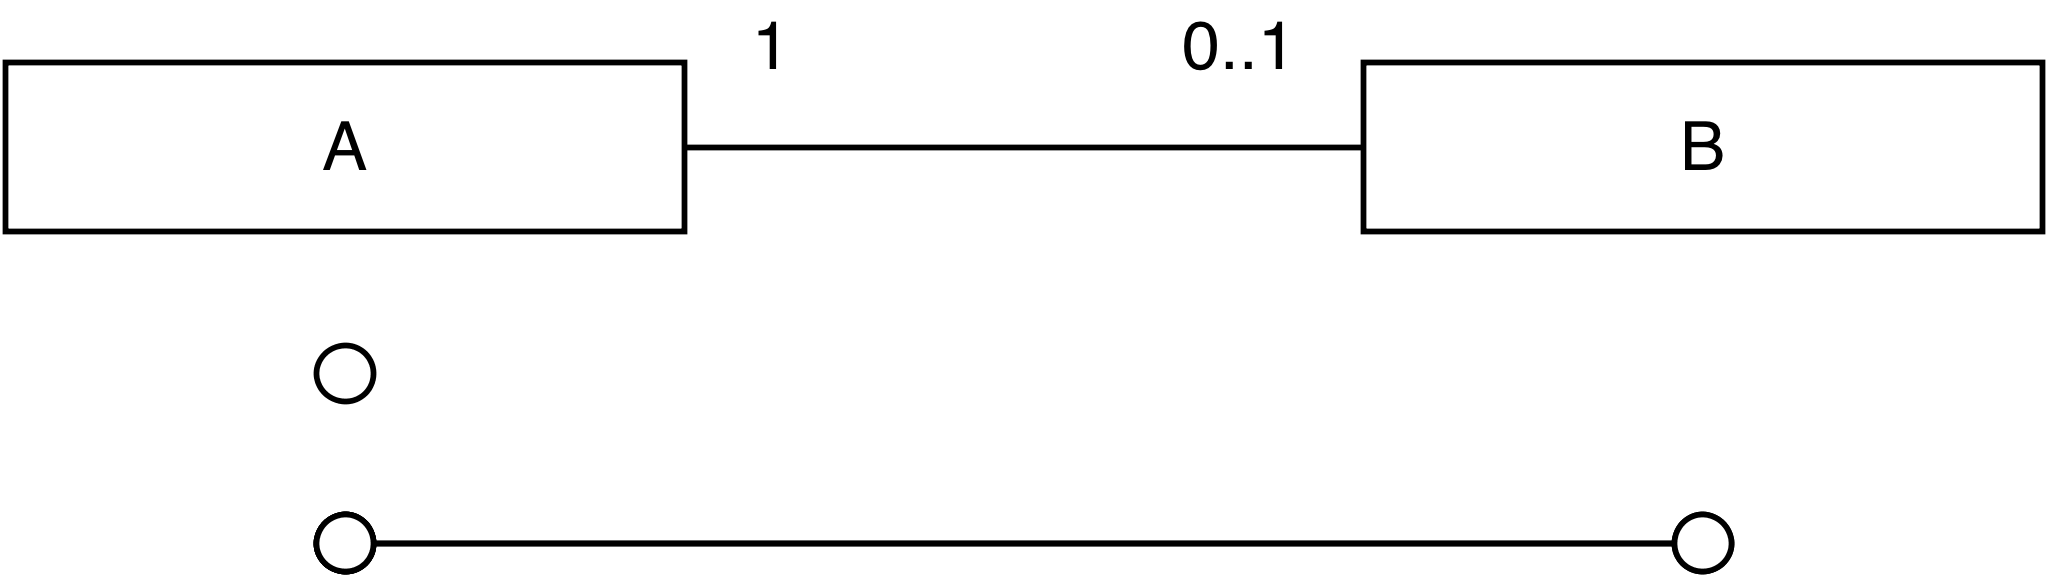
\includegraphics[width=0.55\textwidth]{images/generierung/nm-1-to-0-1.png}
  	  \caption{Beziehungen nach dem Schema 1:0..1 (n:m)}\label{img:generierung:1to01}
  	\end{figure}		
		
		
		\subsubsection{2. Fall (n:M): 1:4}
		
		Der zweite Fall betrachtet eine untere mit einer oberen Grenze. Die in diesem Beispiel erzeugten Entit�ten zeigt
		Abbildung \ref{img:generierung:1to4}.
		
	  \begin{figure}[htbp]
  	  \centering
  	   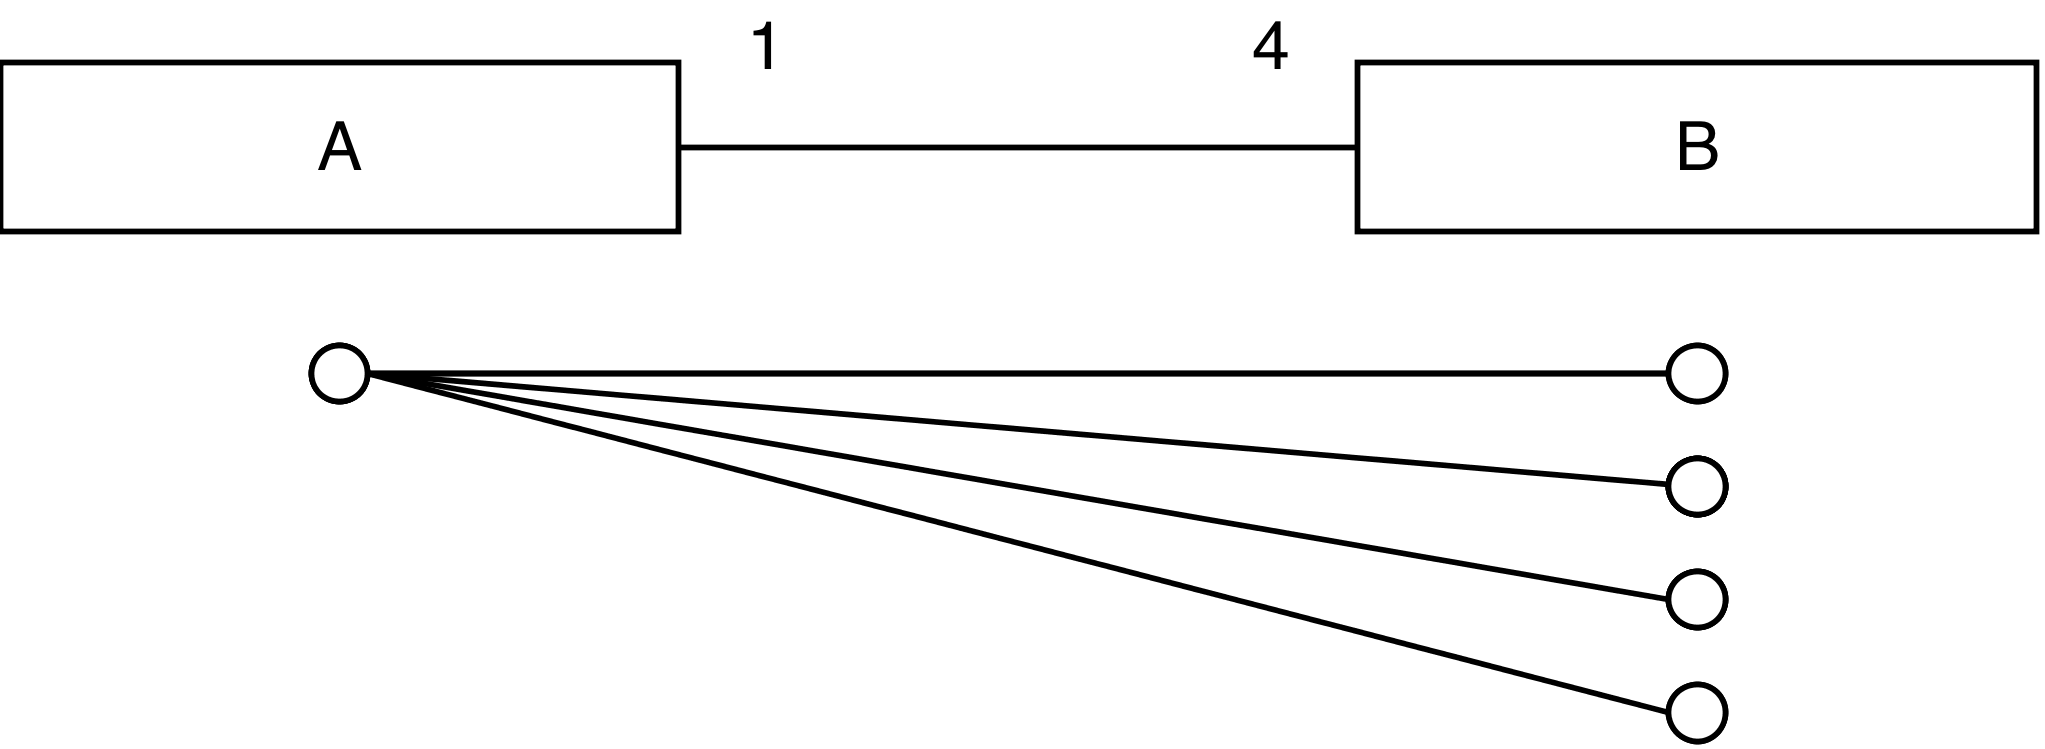
\includegraphics[width=0.55\textwidth]{images/generierung/nm-1-to-4.png}
  	  \caption{Beziehungen nach dem Schema 1:4 (n:M)}\label{img:generierung:1to4}
  	\end{figure}		

		\subsubsection{3. Fall (N:m): 3:0..1}
		
		Wie im ersten Fall ist hier eine der beiden Grenzen 0. Die in der Abbildung \ref{img:generierung:3to01} dargestellte 
		Entit�t ohne Beziehung ist der Vollst�ndigkeit halber aufgezeigt, muss aber nicht generiert werden, da sie bereits 
		generiert wurde (siehe Abbildung \ref{img:generierung:1to01}).
		
	  \begin{figure}[htbp]
  	  \centering
  	   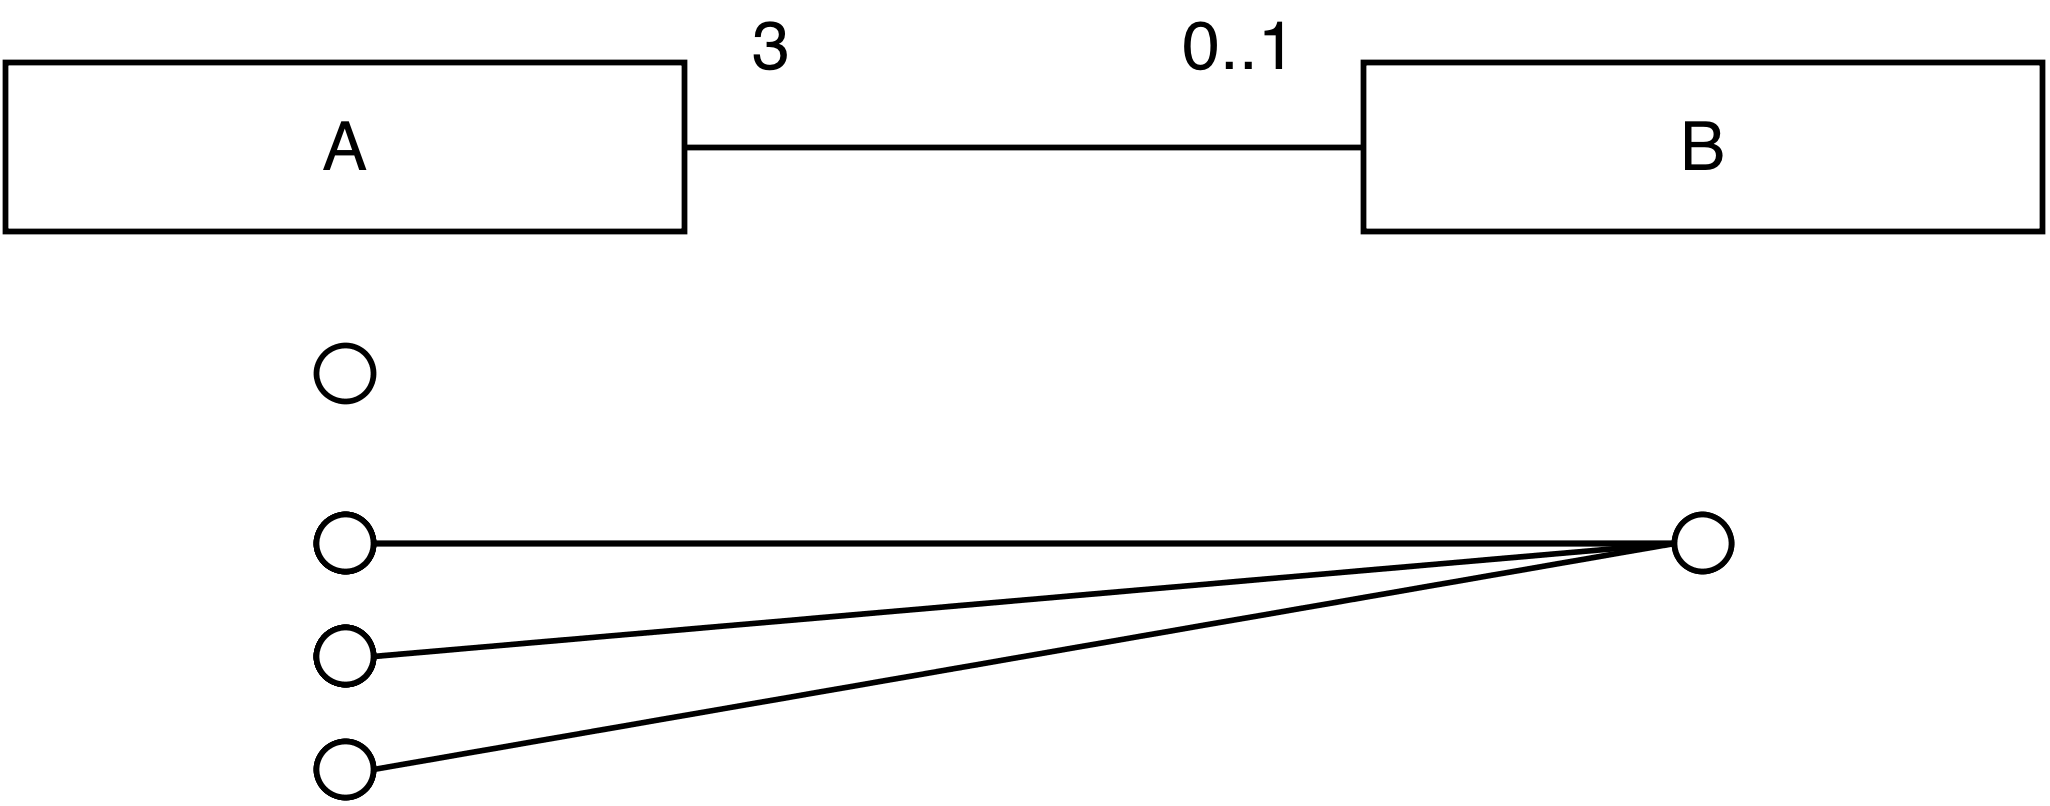
\includegraphics[width=0.55\textwidth]{images/generierung/nm-3-to-0-1.png}
  	  \caption{Beziehungen nach dem Schema 3:0..1 (N:m)}\label{img:generierung:3to01}
  	\end{figure}		

		\subsubsection{4. Fall (N:M): 3:4}
		
		Der vierte Fall behandelt schlie�lich die beiden oberen Grenzen. Abbildung \ref{img:generierung:3to4} zeigt die
		Vollvermaschung der zu erzeugenden Entit�ten.
	
	  \begin{figure}[htbp]
  	  \centering
  	   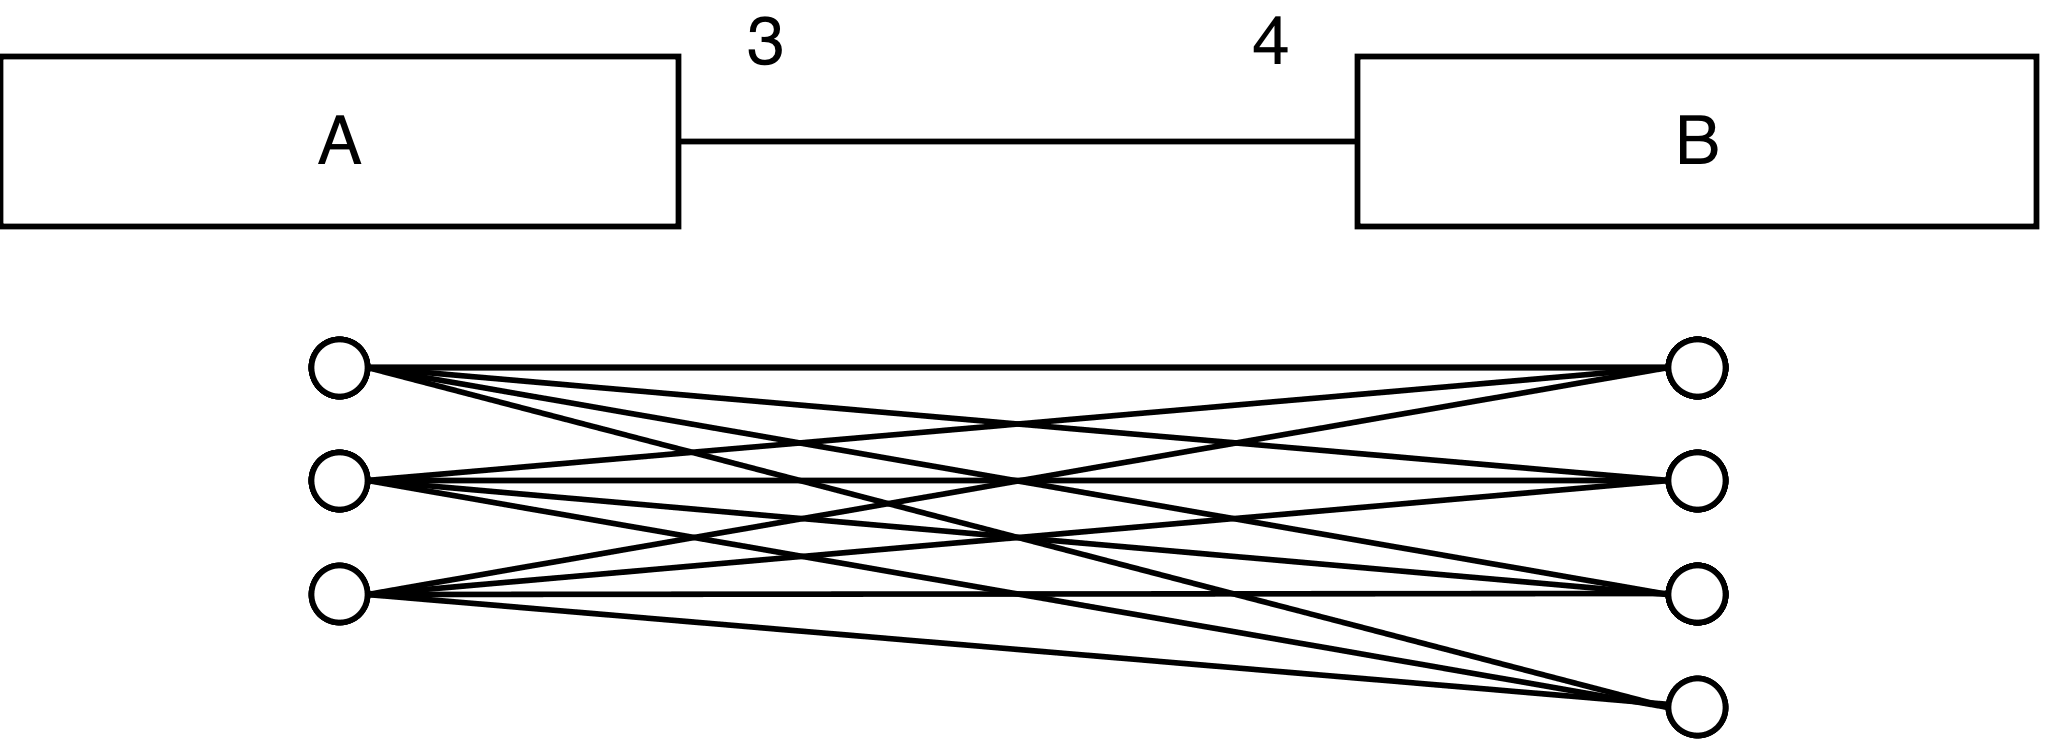
\includegraphics[width=0.55\textwidth]{images/generierung/nm-3-to-4.png}
  	  \caption{Beziehungen nach dem Schema 3:4 (N:M)}\label{img:generierung:3to4}
  	\end{figure}

		\subsubsection{Gesamte Generierung (n..N:m..M): 1..3:0..4}
		
		F�r eine Beziehung nach dem Schema 1..3:0..4 w�rde der Algorithmus die in Abbildung \ref{img:generierung:13to04}
		dargestellte Entit�ten und Beziehungen vorsehen.
		
	  \begin{figure}[htbp]
  	  \centering
  	   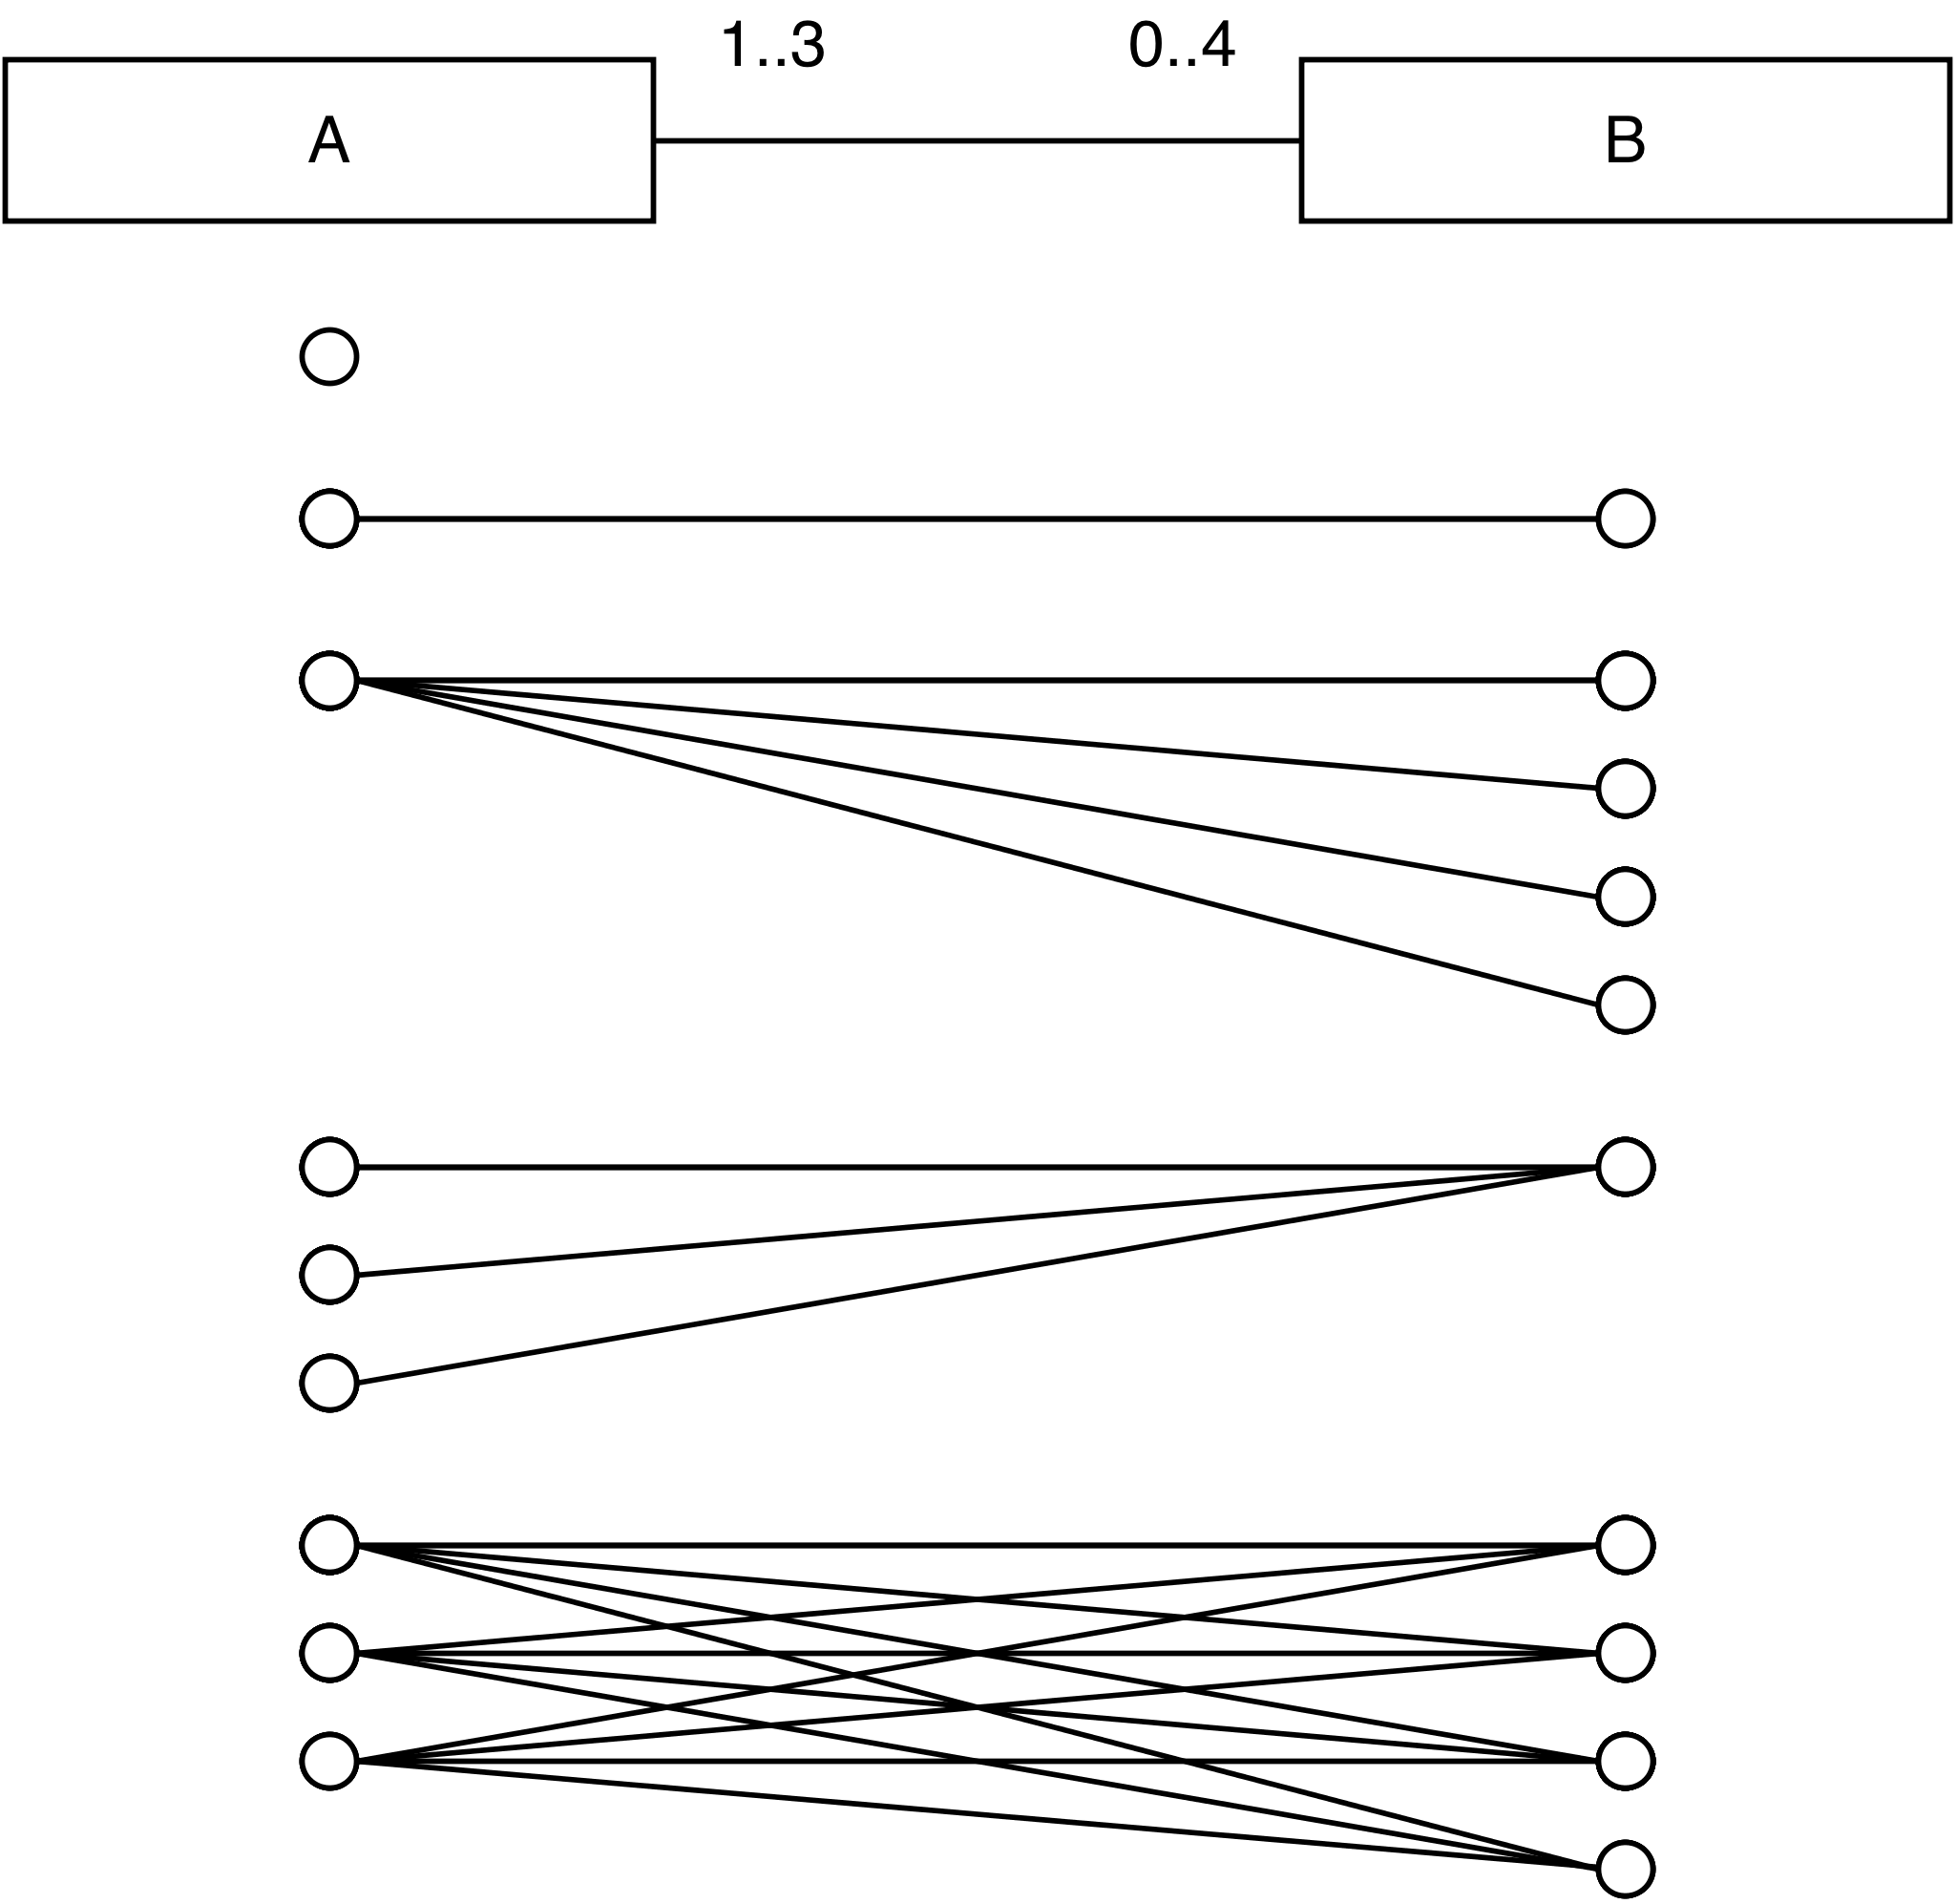
\includegraphics[width=0.55\textwidth]{images/generierung/nm-1-3-to-0-4.png}
  	  \caption{Beziehungen nach dem Schema 1..3:0..4 (n..N:m..M)}\label{img:generierung:13to04}
  	\end{figure}

\section{Komplexit�t bei der Generierung von Beziehungen}
\label{sec:generieren:komplexitaet}

Im vorausgegangenen Abschnitt wurden nur Beziehungen zwischen zwei Entit�tstypen betrachtet. In realen Anwendungen k�nnen
Entit�tstypen mit mehr als nur einem anderen Entit�tstyp in Beziehung stehen und auch mit dem selben Entit�tstyp mehr als
nur ein Mal.

Bez�glich der Datengenerierung lassen sich hierbei zwei generelle Vorgehensweisen lassen sich hier unterscheiden:
\begin{itemize}
	\item \textbf{Beziehungen unabh�ngig betrachten}: Es wird angenommen, dass unterschiedliche Beziehungen voneinander
	  unabh�ngig sind. Die Frage, ob ein Professor eine Lehrveranstaltung leitet, l�sst keine R�ckschl�sse zu, ob und welche
		Pr�fungen er beaufsichtigt.
	
	\item \textbf{Beziehungen abh�ngig voneinander betrachten}: In der Praxis beeinflussen sich viele Beziehungen. Ein Student,
	  der die Pr�fung einer Lehrveranstaltung schreibt, darf wohl nicht gleichzeitig Tutor dieser Veranstaltung sein.
	
\end{itemize}

Alle Beziehungen abh�ngig voneinander zu betrachten kann schnell zu exponentiell zunehmenden Testdaten f�hren. 
Einen riesigen Bestand an Daten um f�r Tests unn�tige Beziehungen und schlie�lich auch Entit�ten zu verringern
scheint aufw�ndiger, als einen kleinen Datenbestand um fehlende Beziehungen punktuell zu erweitern. Aus diesem Grund
ber�cksichtigt der Algorithmus keine Beziehungen in Abh�ngigkeit von anderen -- mit Ausnahme von assoziativen
Tabellen.

\section{Algorithmus zur Generierung von Beziehungen}
\label{sec:generieren:algorithmus}

Der entwickelte Algorithmus �bernimmt aus \cite{Houkjaer:2006:SRD:1182635.1164254} die Idee, das Modell als Graphen
zu betrachten und zu traversieren. Bevor der Pseudocode des Algorithmus beschrieben wird, werden einige verwendete
Begriffe beschrieben und das Klassen-Diagramm des Modells vorgestellt, das der Daten-Generator verwendet.

	\subsection{Begriffserkl�rungen}
  Die Beschreibung des Algorithmus verwendet einige Begriffe und Konventionen, die im Folgenden beschrieben werden.
	
		\subsubsection{Knoten und Kanten}
		
		Die Idee, das Datenbank-Modell als Graphen zu betrachten, stammt aus \cite{Houkjaer:2006:SRD:1182635.1164254}. 
		Tabellen stellen die Knoten des Graphs dar. Die Foreign-Key-Beziehungen zwischen zwei Tabellen stellen die Kanten
		des Graphs dar. Eine Kante ist gerichtet, von der Tabelle mit der Foreign-Key-Spalte zur referenzierten Tabelle hin.
		Aufgrund der Richtung hat jede Kante eine Start- und eine Zieltabelle.
		
		Auch wenn es sich um gerichtete Kanten handelt, ist eine Traversierung in beide Richtungen m�glich.
		
	
		\subsubsection{Assoziative Tabellen}
		
		Assoziative Tabellen verbinden zwei Tabellen. Die beiden verbundenen Tabellen werden im Folgenden als linke und rechte
		Tabelle bezeichnet, analog wird von linker und rechter Kante gesprochen.
		
		Die Reihenfolge, in der die Spalten der Tabelle definiert sind, bestimmt die Einteilung in links und rechts. Der erste
		Fremdschl�ssel referenziert die linke Tabelle. Das Ergebnis der Generierung h�ngt jedoch nicht von dieser Einteilung ab.
	
  \subsection{Klassendiagramm}
	
	
	
	
	
	

  \subsection{Pseudocode}
  \label{sec:generieren:algorithmus:pseudocode}
	
	Der Algorithmus ist in mehrere Teilfunktionen unterteilt. Einige Funktionen werden rekursiv aufgerufen, um den Graphen
	entlang der Kanten zu traversieren. Der Einstiegspunkt stellt die Funktion \texttt{Generiere\_Test\_Daten} dar, die im
	folgenden Abschnitt beschrieben wird.
	
		\subsubsection{Generiere Test-Daten}
		
		Die Funktion \texttt{Generiere\_Test\_Daten} (siehe Listing \ref{listing:GeneriereTestDaten}) ist der Einstiegspunkt
		f�r den Algorithmus zur Generierung von Test-Daten.
		Im ersten Schritt wird die Reihenfolge der Tabellen festgelegt, die als Startpunkte in Frage kommen. Die Liste
		stellt sicher, dass auch Datenbank-Modelle, die aus mehreren unabh�ngigen Graphen bestehen, vollst�ndig
		generiert werden. In einem Datenbank-Modell, in dem alle Tabellen direkt oder indirekt in Beziehung stehen,
		w�rde die Festlegung einer Starttabelle ausreichen.
		
		Zur Sortierung der Tabellen wird die Anzahl eingehender Kanten verwendet. Der Grund daf�r und die Bedeutung der
		Reihenfolge der Tabellen wird in Abschnitt \ref{sec:generieren:evaluation:tabellenreihenfolge} beschrieben.
		
		Anschlie�end wird �ber diese Tabellenliste iteriert. Wurde eine Tabelle noch nicht behandelt, wird die
		entsprechende Funktion zur Generierung der Daten aufgerufen. Dabei werden nicht-assoziative und
		assoziative Tabellen unterschiedlich behandelt. Der Grund daf�r ist, dass assoziative Tabellen ein
		Hilfskonstrukt darstellen, das selbst eine Beziehung auf ER-Ebene darstellt.
		
		Am Ende stellt der Algorithmus sicher, dass jede Entit�t g�ltig generiert wurde, also dass die Beziehungen
		die Constraints erf�llen. Gegebenenfalls werden hier Entit�ten nach generiert.
  
\begin{lstlisting}[caption=Generiere Test-Daten, label=listing:GeneriereTestDaten]
GeneriereTestDaten
------------------
L := Tabellenliste, nach Anzahl eingehender Kanten aufsteigend geordnet
FOR EACH (noch nicht besuchte Tabelle T IN der geordneten Tabellenliste L)
DO
  Markiere Tabelle T als besucht;
  IF (Tabelle T ist keine assoziative Tabelle)
  THEN CALL Generiere_Daten_Fuer_Nichtassoziative_Tabelle(T);
  ELSE CALL Generiere_Daten_Fuer_Assoziative_Tabelle(T);
  END IF;
END FOR;
CALL Erweitere_Generierte_Daten_Zu_Konsistenten_Daten()
\end{lstlisting}

		\subsubsection{Generiere Daten f�r nichtassoziative Tabelle}
		
		Der Generator betrachtet zur Generierung von Entit�ten die Beziehungen der Tabellen. Aus diesem Grund
		erzeugt die Funktion \texttt{Generiere\_Daten\_Fuer\_Nichtassoziative\_Tabelle}
		(siehe Listing \ref{listing:GeneriereDatenFuerNichtassoziativeTabelle})
		selbst keine Daten. Stattdessen werden die (noch unbehandelten) Kanten der Tabelle betrachtet. 
		
		Handelt es sich bei der an der Beziehung beteiligten Tabelle um eine assoziative Tabelle, wird mit der
		Generierung der assoziativen Beziehungen fortgesetzt. Ansonsten wird die Funktion zur Generierung der
		Daten f�r eine Kante aufgerufen.
		
	  Der Algorithmus aus \cite{Houkjaer:2006:SRD:1182635.1164254} bevorzugt ausgehende Kanten bei der Erzeugung
		von Daten, da sich diese mit weniger Aufwand abarbeiten lassen. Diese Bevorzugung wird f�r den hier
		entwickelten Algorithmus �bernommen, auch wenn sich der Aufwand f�r ein- und ausgehende Kanten nicht
		unterscheidet.

\begin{lstlisting}[caption=GeneriereDatenFuerNichtassoziativeTabelle, label=listing:GeneriereDatenFuerNichtassoziativeTabelle]
Generiere_Daten_Fuer_Nichtassoziative_Tabelle(Tabelle T)
---------------------------------------------------
FOR EACH (ausgehende Kante K, die noch nicht besucht wurde)
DO
  IF (Zieltabelle Z von Kante K ist keine assoziative Tabelle)
  THEN Markiere Kante K als besucht;
       CALL Generiere_Daten_Fuer_Kante(K);
			 IF (Zieltabelle Z noch nicht besucht) 
			 THEN Markiere Tabelle Z als besucht;
            CALL Generiere_Daten_Fuer_Nicht_Assoziative_Tabelle(Z);
			 END IF;
  ELSE CALL Generiere_Daten_Fuer_Assoziative_Tabelle(Z);
  END IF;
END FOR;
FOR EACH (eingehende Kante K, die noch nicht besucht wurde)
DO
  IF (Starttabelle S von Kante K ist keine assoziative Tabelle)
  THEN Markiere Kante K als besucht;
       CALL Generiere_Daten_Fuer_Kante(K);
			 IF (Starttabelle S noch nicht besucht) 
			 THEN Markiere Tabelle S als besucht;
            CALL Generiere_Daten_Fuer_Nicht_Assoziative_Tabelle(S);
			 END IF;
  ELSE CALL Generiere_Daten_Fuer_Assoziative_Tabelle(S);
  END IF;
END FOR;
\end{lstlisting}

		\subsubsection{Generiere Daten f�r Kante}
		
		Die Funktion zum Generieren von Daten f�r eine Kante setzt die f�hrt die 
		\ref{sec:generieren:beziehungen:nm} beschriebenen Schritte um (siehe Listing \ref{listing:GeneriereDatenFuerKante}). 
		Es werden alle vier Kombinationen aus Minimum und Maximum behandelt (Zeilen 6-9). Die eigentliche Generierung findet
		ist in eine Hilfsfunktion ausgelagert, die mit allen Min-Max-Kombinationen aufgerufen wird.

\begin{lstlisting}[caption=Generiere Daten Fuer Kante, label=listing:GeneriereDatenFuerKante]
Generiere_Daten_Fuer_Kante(Kante K)   
------------------------------
S := Starttabelle von Kante K;
Z := Zieltabelle von Kante K;
// Generierung der Daten entsprechend Abschnitt 6.2.3
CALL Generiere_Entitaeten_Und_Beziehungen(K, min(S), min(Z));
CALL Generiere_Entitaeten_Und_Beziehungen(K, min(S), max(Z));
CALL Generiere_Entitaeten_Und_Beziehungen(K, max(S), min(Z));
CALL Generiere_Entitaeten_Und_Beziehungen(K, max(S), max(Z));
\end{lstlisting}

		\subsubsection{Generiere Entit�ten und Beziehungen}
		
		Es soll vermieden werden, unn�tige Entit�ten und Beziehungen zu generieren. Unn�tig sind vor allem
		redundante Beziehungen. Diese k�nnen beispielsweise entstehen, wenn die untere und die obere Grenze einer
		Multiplizit�t identisch sind. Deshalb wird f�r jede Kombination aus Kante, Anzahl der beteiligten Entit�ten
		der Starttabelle und Anzahl der beteiligten Entit�ten der Zieltabelle die Generierung nur ein einziges
		Mal durchgef�hrt.
		
		Der Algorithmus (siehe Listing \ref{listing:GeneriereEntitaetenUndBeziehungen}) pr�ft, ob es sich um eine
		optionale Beziehung handelt (Zeile 7 und Zeile 10). Eine der Grenzen s bzw. z
		ist in einem solchen Fall gleich 0. Handelt es sich um eine optionale Beziehung, wird eine entsprechende
		Entit�t berechnet, die in Bezug auf die Kante in keiner Beziehung ist. Anschlie�end wird die Funktion
		rekursiv aufgerufen, diesmal mit dem Wert 1 als Grenze anstelle der 0 (Zeile 9 und Zeile 12).
		
		Sofern s und z beide ungleich 0 sind, wird eine Entit�t in der Zieltabelle berechnet und s Entit�ten 
		in der Starttabelle. Zwischen diesen Entit�ten wird die von der Kante K repr�sentierte Beziehung
		hergestellt (Zeilen 14 bis 19).
		
		Der Eingangswert z kann aufgrund der Tatsache, dass es sich um eine nicht-assoziative Tabelle handelt,
		nur 0 oder 1 sein.
		
\begin{lstlisting}[caption=Generiere Entit�ten Und Beziehungen, label=listing:GeneriereEntitaetenUndBeziehungen]
Generiere_Entitaeten_Und_Beziehungen(K, s, z)
-----------------------------------------
// Sicherstellen, dass nicht mehr Entit�ten als notwendig erzeugt werden
IF (F�r die Kombination (K, s, z) wurden bereits Entit�ten erzeugt) 
THEN RETURN;
END IF
IF (Wert der Grenze s ist 0)
THEN Berechne Entit�t e in Zieltabelle, die in keiner Beziehung zur Starttabelle stehen darf;
     CALL Generiere_Entitaeten_Und_Beziehungen(k, 1, z);
ELSE IF (Wert der Grenze z ist 0)
THEN Berechne Entit�t e in Starttabelle, die in keiner Beziehung zur Zieltabelle stehen darf;
     CALL Generiere_Entitaeten_Und_Beziehungen(k, s, 1);
ELSE // z ist hier immer 1
     Berechne Entit�t e in Zieltabelle, die in keiner Beziehung zur Starttabelle stehen darf;
		 FOR i = 1 TO s
		 DO 
       Berechne Entit�t se in Starttabelle, die in keiner Beziehung zur Zieltabelle stehen darf;
		   Stelle Beziehung zwischen Entit�t se und Entit�t e her;
		 END FOR;
END IF;
\end{lstlisting}

		\subsubsection{Generiere Daten f�r assoziative Tabelle}
		
		Assoziative Tabellen werden typischerweise zur Modellierung von n..N:m..M-Beziehungen verwendet. Diese Beziehungen
		werden entsprechend der in Abschnitt \ref{sec:generieren:beziehungen:nm} beschriebenen Strategie generiert. D.h. es
		werden alle vier Kombinationen aus den jeweiligen Minimal- und Maximalwerten betrachtet.
		
		Nach der Erzeugung der Daten f�r die assoziative Tabelle versucht der Algorithmus (siehe 
		Listing \ref{listing:GeneriereDatenFuerAssoziativeTabelle}), die Generierung bei den beiden
		assoziierten Tabellen fortzusetzen -- falls diese noch nicht behandelt wurden.

\begin{lstlisting}[caption=Generiere Daten f�r assoziative Tabelle, label=listing:GeneriereDatenFuerAssoziativeTabelle]
Generiere_Daten_Fuer_Assoziative_Tabelle(Tabelle T)
-----------------------------------------------
LK := linke Kante der assoziativen Tabelle T;
RK := rechte Kante der assoziativen Tabelle T;
markiere Kanten LK und RK als besucht;
LM := Multiplizit�t der linken Beziehung, ausgehende Seite
RM := Multiplizit�t der rechten Beziehung, ausgehende Seite
CALL Generiere_Assoziative_Entitaeten_Und_Beziehungen(T, min(LM), min(RM));
CALL Generiere_Assoziative_Entitaeten_Und_Beziehungen(T, min(LM), max(RM));
CALL Generiere_Assoziative_Entitaeten_Und_Beziehungen(T, max(LM), min(RM));
CALL Generiere_Assoziative_Entitaeten_Und_Beziehungen(T, max(LM), max(RM));
LT := Zieltabelle von Kante LK;
RT := Zieltabelle von Kante RK;
IF (LT wurde noch nicht besucht)
THEN Markiere Tabelle LT als besucht;
     IF (Tabelle LT ist keine assoziative Tabelle)
     THEN CALL Generiere_Daten_Fuer_Nichtassoziative_Tabelle(LT);
     ELSE CALL Generiere_Daten_Fuer_Assoziative_Tabelle(LT);
     END IF;
END IF;
IF (RT wurde noch nicht besucht)
THEN Markiere Tabelle RT als besucht;
     IF (Tabelle RT ist keine assoziative Tabelle)
     THEN CALL Generiere_Daten_Fuer_Nichtassoziative_Tabelle(RT);
     ELSE CALL Generiere_Daten_Fuer_Assoziative_Tabelle(RT);
     END IF;
END IF;
\end{lstlisting}

		\subsubsection{Generiere assoziative Entit�ten und Beziehungen}
		
		Die Funktion \texttt{Generiere\_Assoziative\_Entitaeten\_Und\_Beziehungen} erzeugt Entit�ten und Beziehungen
		in Verbindung mit assoziativen Tabellen (siehe Listing \ref{listing:GeneriereAssoziativeEntitaetenUndBeziehungen}).
		D.h. sie erzeugt Entit�ten in der assoziativen Tabelle und bei Bedarf in den beiden an der Assoziation beteiligten
		Tabellen (linke und rechte Tabelle der assoziativen Tabelle).
		
		Die Funktion erwartet drei Parameter:
		\begin{itemize}
			\item \textbf{Tabelle \texttt{AT}}: Die assoziative Tabelle, die behandelt wird.

			\item \textbf{Grenze \texttt{l}}: Der momentane Grenzwert der linksseitigen Multiplizit�t.

			\item \textbf{Grenze \texttt{r}}: Der momentane Grenzwert der rechtsseitigen Multiplizit�t.
		\end{itemize}
		
		Abbildung \ref{img:generierung:tauschat} veranschaulicht die Parameter und zeigt, dass die angegebenen Grenzen
		bestimmen, wie viele Entit�ten der \textit{anderen} Tabelle ben�tigt werden. D.h. \texttt{l} bestimmt, wie viele
		Entit�ten der rechten Tabelle, und \texttt{r} bestimmt, wie viele Entit�ten der linken Tabelle generiert werden
		m�ssen.
		
	  \begin{figure}[htbp]
  	  \centering
  	   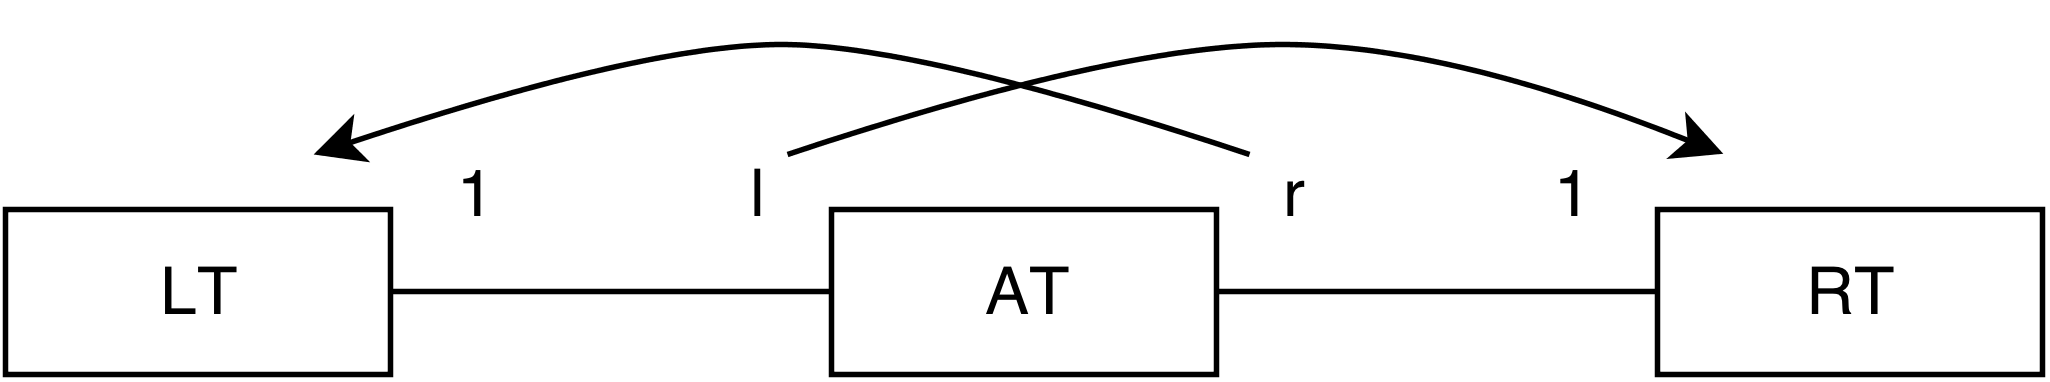
\includegraphics[width=0.55\textwidth]{images/generierung/tausch-at.png}
  	  \caption{Parameter f�r Daten-Generierung bei assoziativer Tabelle}\label{img:generierung:tauschat}
  	\end{figure}
		
		F�r den Fall dass \texttt{l} oder \texttt{r} den Wert 0 enthalten, wird eine entsprechende Entit�t in der
		rechten bzw. linken Tabelle berechnet, die keine Beziehung zur assoziativen Tabelle \texttt{AT} hat. 
		In den Zeilen 6 und 10 wird die Anzahl der zu berechnenden Entit�ten der linken Tabelle (Variable \texttt{LA})
		und der rechten Tabelle (Variable \texttt{RA}) berechnet. Als Minimalwert wird wie schon vorher bei
		optionalen Beziehungen der Wert 1 verwendet.
		
		Sollten f�r die Kombination \texttt{LA} und \texttt{RA} f�r die assoziative Tabelle \texttt{AT} bereits
		Daten generiert worden sein, bricht die Funktion an dieser Stelle ab (Zeilen 14 und 15). Ein solcher Fall
		kann eintreten, wenn untere und obere Grenze einer Multiplizit�t identisch sind, oder es eine Multiplizit�t
		der Form 0..1 ist.
		
		Der Algorithmus berechnet zuerst alle Entit�ten in der linken (Zeilen 17 bis 20) und dann in der
		rechten Tabelle (Zeilen 21 bis 24). Danach werden die Entit�ten in der assoziativen Tabelle erzeugt
		und die Beziehungen hergestellt (Zeilen 25 bis 33).
		

\begin{lstlisting}[caption=Generiere Assoziative Entitaeten Und Beziehungen, label=listing:GeneriereAssoziativeEntitaetenUndBeziehungen]
Generiere_Assoziative_Entitaeten_Und_Beziehungen(AT, l, r)
----------------------------------------------------
LK := linke Kante der assoziativen Tabelle AT;
RK := rechte Kante der assoziativen Tabelle AT;
// Grenzen "tauschen" und Mindestanzahl auf 1
LA := Max(r, 1);  // r als Grenze f�r linke Tabelle, mindestens 1
IF (r ist gleich 0) 
THEN Berechne Entit�t in linker Tabelle, die in keiner Beziehung zur assoziativen Tabelle AT stehen darf;
ENDIF;
RA := Max(l, 1);  // l als Grenze f�r rechte Tabelle, mindestens 1
IF (l ist gleich 0) 
THEN Berechne Entit�t in rechter Tabelle, die in keiner Beziehung zur assoziativen Tabelle AT stehen darf;
ENDIF;
IF (F�r die Kombination (AT, LA, RA) wurden bereits Entit�ten erzeugt) 
THEN RETURN;
END IF
FOR i = 1 TO RA
DO 
  Berechne Entit�t le[i] in linker Tabelle, die in keiner Beziehung zur assoziativen Tabelle AT stehen darf;
END FOR;
FOR j = 1 TO LA
DO 
  Berechne Entit�t re[j] in rechter Tabelle, die in keiner Beziehung zur assoziativen Tabelle AT stehen darf;
END FOR;
FOR i = 1 TO RA
DO 
  FOR j = 1 TO LA
  DO 
    Erzeuge Entit�t e in assoziativer Tabelle AT;
    Stelle Beziehung zwischen Entit�t e und Entit�t le[i] her;
	  Stelle Beziehung zwischen Entit�t e und Entit�t re[j] her;
  END FOR;
END FOR;
\end{lstlisting}

		\subsubsection{Erweitere Generierte Daten zu konsistenten Daten}
		
		Es kann passieren, dass am Ende der Traversierung des Graphs ung�ltige Entit�ten vorhanden sind.
		Ung�ltig bedeutet, dass sie bei eine oder mehrere Kanten nicht in ausreichend vielen Beziehungen steht.
		Dies kann passieren, wenn f�r eine bereits besuchte Tabelle zus�tzliche Entit�ten erzeugt werden
		m�ssen -- beispielsweise wenn das Datenbank-Modell zirkul�re Abh�ngigkeiten enth�lt.
		
		Der Algorithmus sieht nicht vor, bei zus�tzlicher Erzeugung von Entit�ten den Graphen r�ckw�rts zu
		traversieren. Stattdessen werden am Ende alle Entit�ten validiert und gegebenenfalls wird nachgeneriert.
		
		Die Funktion zur Validierung iteriert �ber die Entit�ten aller Tabellen. Es wird �berpr�ft, ob die
		jeweilige Entit�t g�ltig generiert wurde auf Hinblick der aus- und eingehenden Kanten. Sollte dies f�r
		eine Entit�t nicht der Fall sein, wird eine entsprechende Beziehung hergestellt und die Validierung
		erneut von Anfang an durchgef�hrt.
		
		Listing \ref{listing:ErweitereGenerierteDatenZuKonsistentenDaten} zeigt den Pseudo-Code dieser Funktion.
		
		Es kann passieren, dass diese Funktion niemals beendet wird. Dieses Problem wird in
		Abschnitt~\ref{sec:generieren:offenepunkte:unerfuellbar} thematisiert.
		
\begin{lstlisting}[caption=ErweitereGenerierteDatenZuKonsistentenDaten, label=listing:ErweitereGenerierteDatenZuKonsistentenDaten]
Erweitere_Generierte_Daten_Zu_Konsistenten_Daten()
-------------------------------------------------
FOR EACH (Tabelle T in Tabellenliste)
DO
  FOR EACH (Entit�t e aus generierten Entit�ten der Tabelle T)
	DO
	  FOR EACH (Kante K aus ausgehenden Kanten der Tabelle T)
	  DO
	    IF (e erf�llt Constraints f�r Kante K nicht)
		  THEN Berechne Entit�t f in Zieltabelle der Kante K, die in keiner Beziehung zur Tabelle T stehen darf;
			     Stelle Beziehung zwischen Entit�t e und Entit�t f her;
					 Funktion Erweitere_Generierte_Daten_Zu_Konsistenten_Daten neu starten;
		  END IF;
		END FOR;
	  FOR EACH (Kante K aus eingehenden Kanten der Tabelle T)
	  DO
	    IF (e erf�llt Constraints f�r Kante K nicht)
		  THEN Berechne Entit�t f in Starttabelle der Kante K, die in keiner Beziehung zur Tabelle T stehen darf;
			     Stelle Beziehung zwischen Entit�t e und Entit�t f her;
					 Funktion Erweitere_Generierte_Daten_Zu_Konsistenten_Daten neu starten;
		  END IF;
		END FOR;
	END FOR;
END FOR;
\end{lstlisting}




  \subsection{Beispiel}
	
	Der Algorithmus soll an einem kleinen Beispiel veranschaulicht werden. Dazu wird ein kleines Datenbank-Modell definiert,
	das vier Tabellen enth�lt (siehe Abbildung \ref{img:generierung:examplemodel}). Die Tabelle AT ist assoziativ.
	
	Das Modell l�sst sich auf ER-Ebene folgenderma�en beschreiben:
	Eine Entit�t der Tabelle TABLE1 kann beliebig vielen Entit�ten aus TABLE2 zugeordnet sein. Umgekehrt kann eine Entit�t
	aus TABLE2 entweder einer oder keiner Entit�t aus TABLE1 zugeordnet sein.
	Eine Entit�t aus Tabelle TABLE2 kann mit beliebig vielen Entit�ten aus TABLE3 verbunden sein. Eine Entit�t aus TABLE3
	muss mit mindestens drei und h�chstens f�nf Entit�ten aus TABLE2 in Beziehung stehen.

	\begin{figure}[htbp]
		\centering
		 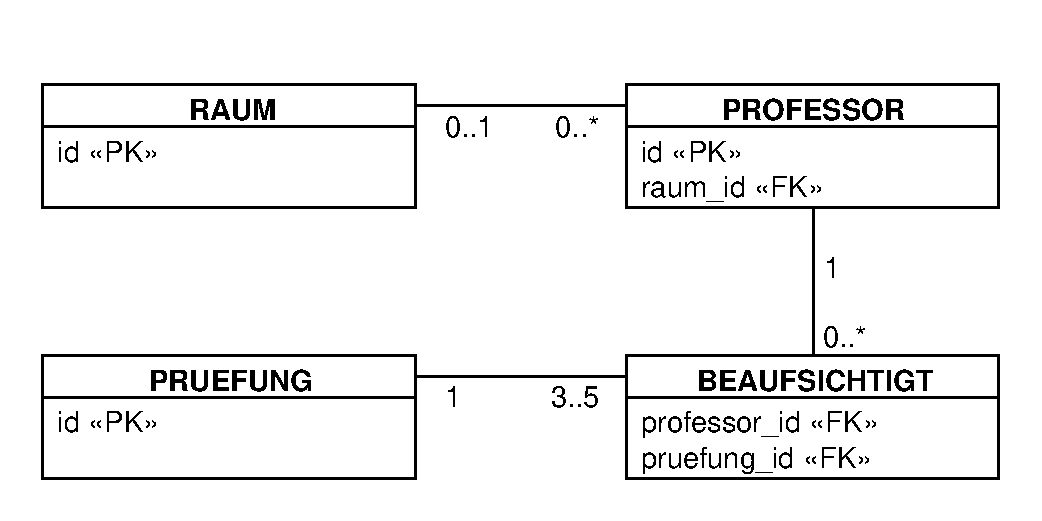
\includegraphics[width=0.55\textwidth]{images/generierung/example_model.pdf}
		\caption{Einfaches Beispiel-Modell f�r den Algorithmus}\label{img:generierung:examplemodel}
	\end{figure}
	
	Als konkreter Wert f�r die offene Grenze \texttt{*} wird der Wert 5 verwendet.
	
  Die generierten Daten f�r das fortlaufende Beispiel befinden sich in Anhang \ref{chap:anhang:generiertedsl}.
	

		\subsubsection{1. Schritt: Sortieren der Tabellen}
		
		Im ersten Schritt werden die Tabellen nach den eingehenden Kanten aufsteigend sortiert. Abbildung
		\ref{img:generierung:examplemodeledges} zeigt die Kanten des Graphen. Die Zahl der eingehenden Kanten ist
		unter der jeweiligen Tabelle vermerkt.

		\begin{figure}[htbp]
			\centering
			 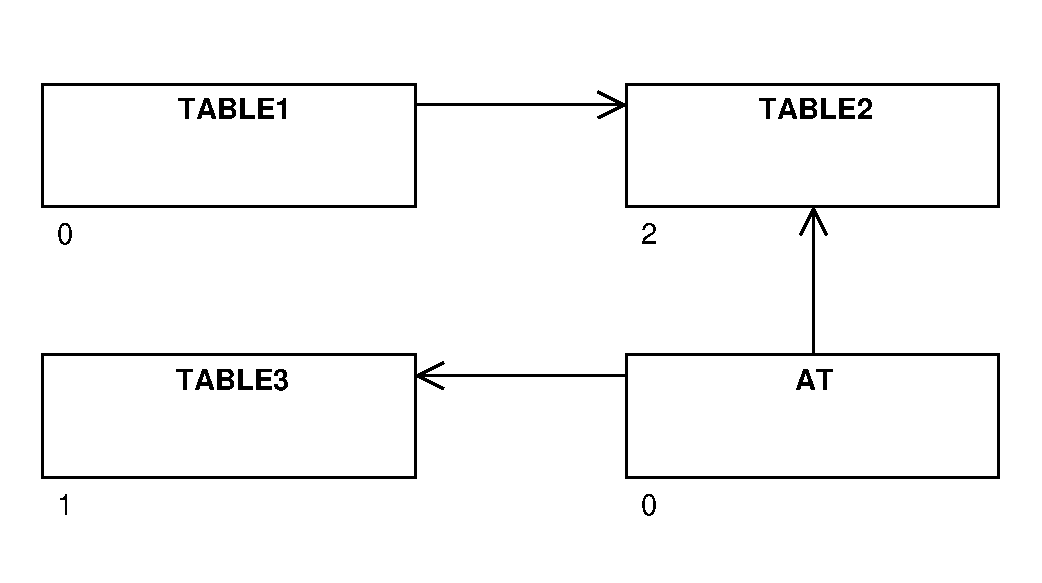
\includegraphics[width=0.55\textwidth]{images/generierung/example_model_edges.pdf}
			\caption{Kanten des einfachen Beispiel-Modells}\label{img:generierung:examplemodeledges}
		\end{figure}
			
	  Da zwei Knoten die selbe Anzahl eingehender Kanten haben, wird als Sekund�rkriterium die Reihenfolge
		der Tabellendefinition verwendet. TABLE1 wurde vor der assoziativen Tabelle AT definiert und ist
		deshalb in der Ordnung weiter oben.
		
		Die sortierte Tabellenliste stellt sich wie folgt dar:
		\begin{enumerate}
			\item \textbf{TABLE1} (0 eingehende Kanten)
			\item \textbf{AT} (0)
			\item \textbf{TABLE3} (1)
			\item \textbf{TABLE2} (2)
		\end{enumerate}
		
		Der Algorithmus iteriert �ber diese Liste und erzeugt ausgehend von der jeweiligen Tabelle
		Daten, sofern die Tabelle nicht bereits behandelt wurde. Die erste Tabelle ist TABLE1.
		
		\subsubsection{2. Schritt: Generierung f�r TABLE1}

    Der Algorithmus befindet sich bei der Generierung bei TABLE1 (siehe Abbildung \ref{img:generierung:example:step_table1}).
		
		\begin{figure}[htbp]
			\centering
			 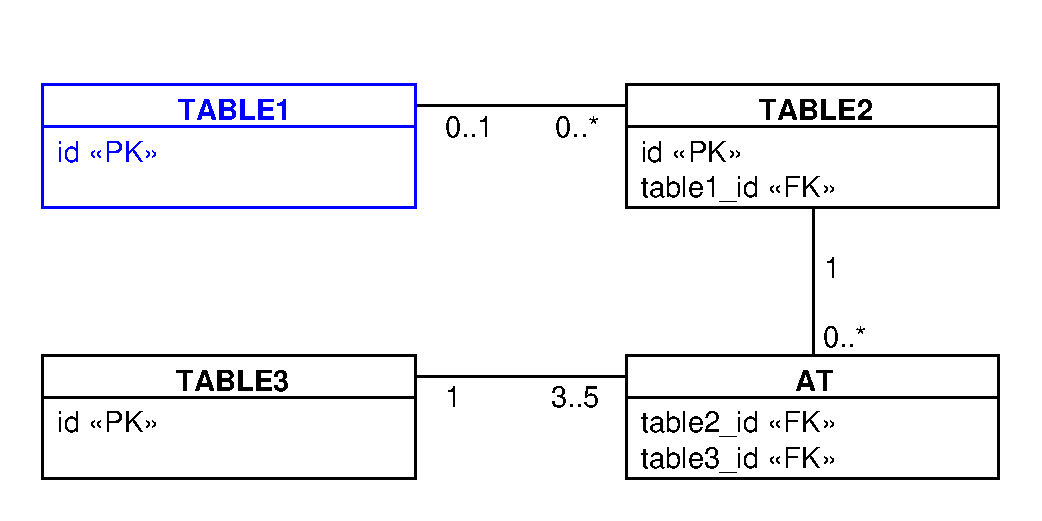
\includegraphics[width=0.55\textwidth]{images/generierung/example_step_table1.pdf}
			\caption{Schritt: TABLE1}\label{img:generierung:example:step_table1}
		\end{figure}

		Es wird �ber die Kanten von TABLE1 iteriert und sofern die Kante noch nicht behandelt wurde,
		werden Daten f�r die jeweilige Kante erzeugt. TABLE1 hat nur eine Kante, diese f�hrt zu TABLE2 und
		wurde noch nicht besucht.
		
		\subsubsection{3. Schritt: Generierung f�r Kante zwischen TABLE1 und TABLE2}
		
		Die Kante repr�sentiert eine 0..1:0..*-Beziehung, die Generierung f�r so eine Kante ist in Abschnitt 
		\ref{sec:generieren:categories:01to0n} beschrieben. Jeweils eine Entit�t steht in keiner Beziehung, 
		zwei Entit�ten befinden sich in einer 1:1-Beziehung und eine Entit�t aus TABLE1 steht mit f�nf
		Entit�ten aus TABLE2 in Beziehung. In der Summe werden damit 3~Entit�ten f�r TABLE1 und 7~Entit�ten
		f�r TABLE2 erzeugt (siehe Tabelle \ref{tab:generierung:table1_table2}).
		
		\begin{table}[ht]
			\caption{Zuordnung der Entit�ten von TABLE1 und TABLE2}
			\centering
			\begin{tabular}{l|l}
				TABLE1     & TABLE2     \\
				\hline
				TABLE1\_1  &            \\
									 & TABLE2\_1  \\
				TABLE1\_2  & TABLE2\_2  \\
				TABLE1\_3  & TABLE2\_3  \\
				TABLE1\_3  & TABLE2\_4  \\
				TABLE1\_3  & TABLE2\_5  \\
				TABLE1\_3  & TABLE2\_6  \\
				TABLE1\_3  & TABLE2\_7  \\
				\hline
				3 Entit�ten  & 7 Entit�ten  \\
			\end{tabular}
			\label{tab:generierung:table1_table2}
		\end{table}
		
		Nachdem die Generierung der Entit�ten und Beziehungen f�r die Kante abgeschlossen ist, setzt der
		Algorithmus die Arbeit bei der Tabelle fort, die mit dieser Kante verbunden ist: TABLE2.

		\subsubsection{4. Schritt: Generierung f�r TABLE2}

		Die Generierung der Daten f�r die Kante zwischen TABLE1 und TABLE2 ist abgeschlossen, TABLE1 ist
		als bereits besuchte Tabelle markiert. Abbildung~\ref{img:generierung:example:step_table2} stellt
		den Generierungsstand grafisch dar.

		\begin{figure}[htbp]
			\centering
			 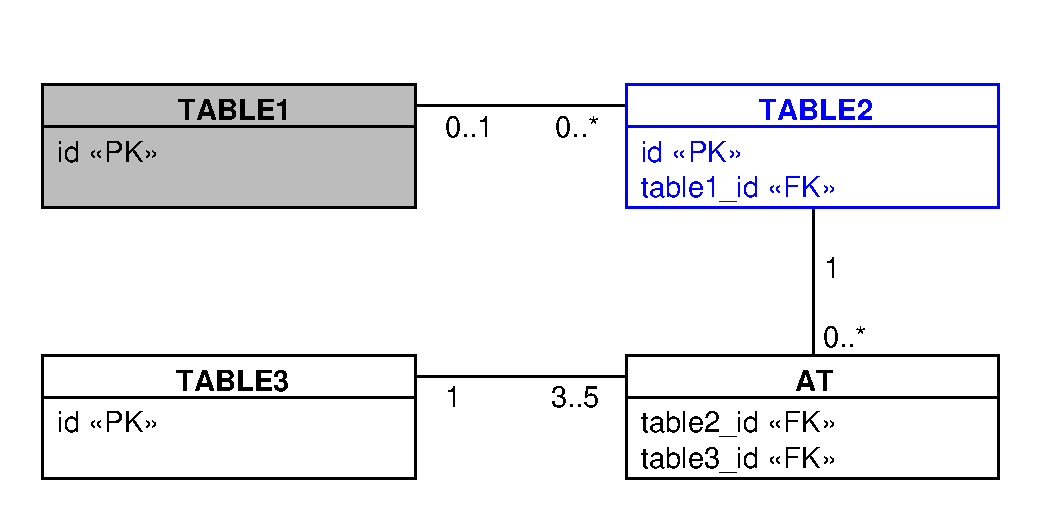
\includegraphics[width=0.55\textwidth]{images/generierung/example_step_table2.pdf}
			\caption{Schritt: TABLE2}\label{img:generierung:example:step_table2}
		\end{figure}
		
		
		Der Algorithmus iteriert �ber die Kanten von TABLE2. Dabei w�rden zuerst ausgehende Kanten betrachtet,
		die Tabelle hat aber nur zwei eingehende. Da die Kante mit TABLE1 bereits besucht wurde, wird die
		Traversierung des Graphs mit der Kante zu Tabelle AT fortgesetzt. Bei AT handelt es sich um eine
		assoziative Tabelle, weshalb der n�chste Schritt die Generierung von Daten f�r die assoziative Tabelle
		AT darstellt.
		
		\subsubsection{5. Schritt: Generierung f�r AT}
		
		Der Daten-Generator befindet sich bei der assoziativen Tabelle AT, die Tabellen TABLE1 und TABLE2
		wurden bereits besucht (siehe Abbildung~\ref{img:generierung:example:step_tableat}).

		\begin{figure}[htbp]
			\centering
			 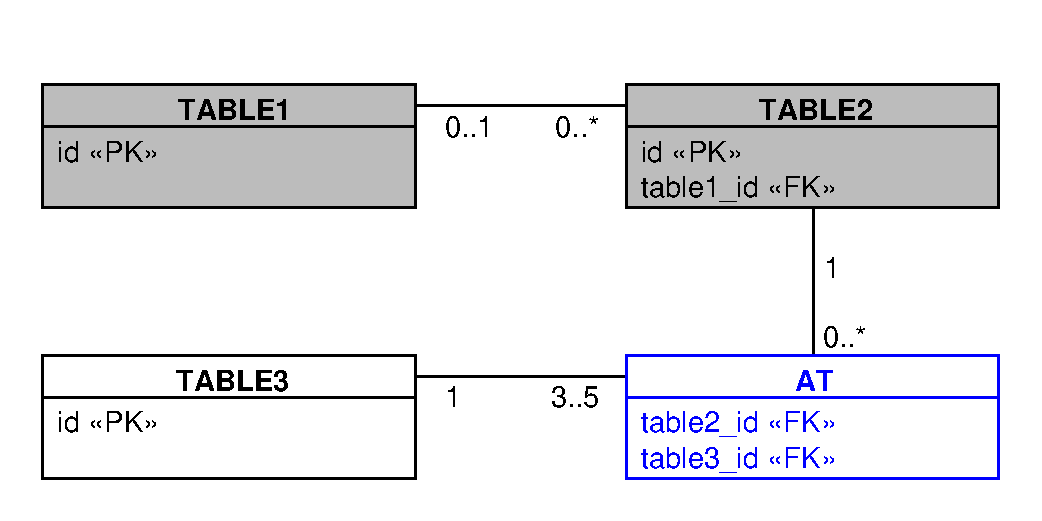
\includegraphics[width=0.55\textwidth]{images/generierung/example_step_tableat.pdf}
			\caption{Schritt: AT}\label{img:generierung:example:step_tableat}
		\end{figure}

		Die assoziative Tabelle AT dient der Modellierung einer 0..*:3..5-Beziehung zwischen den beiden
		Tabellen TABLE2 und TABLE3. Das Generierungsschema f�r assoziative Tabellen ist in 
		Abschnitt~\ref{sec:generieren:beziehungen:nm} beschrieben.
		
    Tabelle~\ref{tab:generierung:table2_table3} zeigt die Zuordnung von Entit�ten aus TABLE2
		und TABLE3. Jedes Paar f�hrt zu einer Entit�t in der Tabelle AT.

		Eine Entit�t aus TABLE2 steht in keiner Beziehung mit Entit�ten aus TABLE3. Jeweils drei 
		und f�nf Entit�ten TABLE2 stehen mit genau einer Entit�t aus TABLE2 in Beziehung (1. und 2. Fall).
		F�nf Entit�ten aus TABLE2 stehen mit drei Entit�ten aus TABLE3 (3. Fall) und weitere f�nf
		Entit�ten aus TABLE2 schlie�lich mit f�nf Entit�ten aus TABLE3 (4. Fall) in Beziehung.
		
		Insgesamt werden f�r die generierten Beziehungen 17~Entit�ten aus TABLE2, 12~Entit�ten aus
		TABLE3 und 48~Entit�ten in der assoziativen Tabelle AT ben�tigt. 7~Entit�ten aus TABLE2
		wurden bereits in Schritt 3 erzeugt, die anderen 10~Entit�ten werden nachgeneriert.
		
		\begin{table}[ht!]
			\caption{Zuordnung der Entit�ten von AT, TABLE2 und TABLE3}
			\centering
			\begin{tabular}{l|l|l||l|l|l}
				AT     & TABLE2     & TABLE3     & AT     & TABLE2     & TABLE3\\
				\hline
	% 0..1:3			                  5:5			
				       & TABLE2\_1  &            & AT\_24 & TABLE2\_13 & TABLE3\_8  \\
				AT\_1  & TABLE2\_2  & TABLE3\_1  & AT\_25 & TABLE2\_13 & TABLE3\_9  \\
				AT\_2  & TABLE2\_3  & TABLE3\_1  & AT\_26 & TABLE2\_13 & TABLE3\_10 \\
				AT\_3  & TABLE2\_4  & TABLE3\_1  & AT\_27 & TABLE2\_13 & TABLE3\_11 \\
	% 0..1:5			
				AT\_4  & TABLE2\_5  & TABLE3\_2  & AT\_28 & TABLE2\_13 & TABLE3\_12 \\
				AT\_5  & TABLE2\_6  & TABLE3\_2  & AT\_29 & TABLE2\_14 & TABLE3\_8  \\
				AT\_6  & TABLE2\_7  & TABLE3\_2  & AT\_30 & TABLE2\_14 & TABLE3\_9  \\
				AT\_7  & TABLE2\_8  & TABLE3\_2  & AT\_31 & TABLE2\_14 & TABLE3\_10 \\
				AT\_8  & TABLE2\_9  & TABLE3\_2  & AT\_32 & TABLE2\_14 & TABLE3\_11 \\
	% 5:3
				AT\_9  & TABLE2\_10 & TABLE3\_3  & AT\_33 & TABLE2\_14 & TABLE3\_12 \\
				AT\_10 & TABLE2\_10 & TABLE3\_4  & AT\_34 & TABLE2\_15 & TABLE3\_8  \\
				AT\_11 & TABLE2\_10 & TABLE3\_5  & AT\_35 & TABLE2\_15 & TABLE3\_9  \\
				AT\_12 & TABLE2\_10 & TABLE3\_6  & AT\_36 & TABLE2\_15 & TABLE3\_10 \\
				AT\_13 & TABLE2\_10 & TABLE3\_7  & AT\_37 & TABLE2\_15 & TABLE3\_11 \\
				AT\_14 & TABLE2\_11 & TABLE3\_3  & AT\_38 & TABLE2\_15 & TABLE3\_12 \\
				AT\_15 & TABLE2\_11 & TABLE3\_4  & AT\_39 & TABLE2\_16 & TABLE3\_8  \\
				AT\_16 & TABLE2\_11 & TABLE3\_5  & AT\_40 & TABLE2\_16 & TABLE3\_9  \\
				AT\_17 & TABLE2\_11 & TABLE3\_6  & AT\_41 & TABLE2\_16 & TABLE3\_10 \\
				AT\_18 & TABLE2\_11 & TABLE3\_7  & AT\_42 & TABLE2\_16 & TABLE3\_11 \\
				AT\_19 & TABLE2\_12 & TABLE3\_3  & AT\_43 & TABLE2\_16 & TABLE3\_12 \\
				AT\_20 & TABLE2\_12 & TABLE3\_4  & AT\_44 & TABLE2\_17 & TABLE3\_8  \\
				AT\_21 & TABLE2\_12 & TABLE3\_5  & AT\_45 & TABLE2\_17 & TABLE3\_9  \\
				AT\_22 & TABLE2\_12 & TABLE3\_6  & AT\_46 & TABLE2\_17 & TABLE3\_10 \\
				AT\_23 & TABLE2\_12 & TABLE3\_7  & AT\_47 & TABLE2\_17 & TABLE3\_11 \\
               &            &            & AT\_48 & TABLE2\_17 & TABLE3\_12 \\
				\hline
               &            &            & 48 Ent. & 17 Entit�ten  & 12 Entit�ten  \\
			 \end{tabular}
			\label{tab:generierung:table2_table3}
		\end{table}
				
		Der Algorithmus hat die Generierung f�r AT abgeschlossen und setzt die Generierung bei
		TABLE3 fort, da TABLE2 bereits besucht wurde.
		
		\subsubsection{6. Schritt: Generierung f�r TABLE3}
		
		Abbildung \ref{img:generierung:example:step_table3} stellt die Ausgangssituation f�r
		den Algorithmus f�r die Generierung von Daten f�r TABLE3 dar. Die Tabellen TABLE1,
		TABLE2 und AT wurden bereits besucht, ebenso die Kanten von TABLE2 nach TABLE1,
		AT nach TABLE2 und AT nach TABLE3.

		\begin{figure}[htbp]
			\centering
			 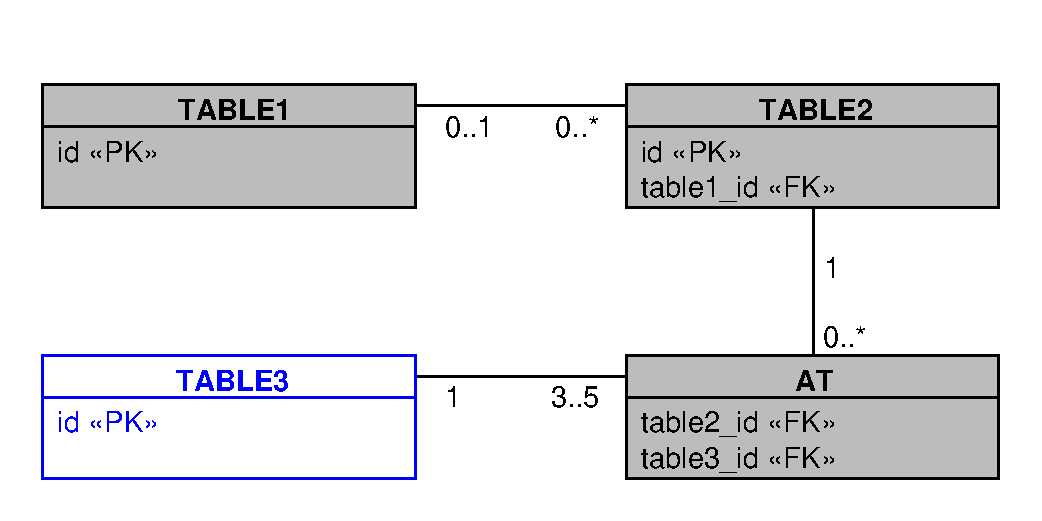
\includegraphics[width=0.55\textwidth]{images/generierung/example_step_table3.pdf}
			\caption{Schritt: Tabelle 3}\label{img:generierung:example:step_table3}
		\end{figure}
		
		Es gibt keine unbesuchten Kanten in TABLE3. Der Algorithmus kehrt zu TABLE2 und
		von dort zu TABLE1 zur�ck, wo ebenfalls keine unbesuchten Kanten mehr sind. In der Liste
		der Tabellen befindet sich auch keine unbesuchten Tabellen mehr, so dass nun der letzte
		Schritt folgt: Die Erweiterung der Daten sofern notwendig.

		\subsubsection{7. Schritt: Erweitern der Daten sofern notwendig}
		
		In diesem Beispiel wurden einige Entit�ten f�r TABLE2 in Schritt 5 nachgeneriert. Da
		diese Entit�ten nur eine optionale Beziehung zu einer Entit�t aus TABLE1 hat, sind die
		nachgenerierten Entit�ten g�ltig. Eine Erweiterung der Daten ist somit nicht notwendig
		und die Generierung abgeschlossen.

\section{Praktischer Einsatz / Evaluation}

  \subsection{Einfluss der Tabellenreihenfolge}
	\label{sec:generieren:evaluation:tabellenreihenfolge}

	Die Art und Weise, wie Beziehungen generiert werden, h�ngen von der Reihenfolge ab, in der die Tabellen und Kanten behandelt
	werden. Die gew�hlte Reihenfolge basiert auf den Kriterien aus \cite{Houkjaer:2006:SRD:1182635.1164254}. Die Sortierung
	wird nicht aus Qualit�tsgr�nden, sondern f�r ein deterministisches Verhalten des Algorithmus beibehalten. Da verschiedene
	Tabellen gleich viele eingehende Kanten haben k�nnen, muss das deterministische Verhalten durch weitere Sortierkritieren
	sichergestellt werden. Dies kann z.B. der Tabellen-Name sein, oder auch die Reihenfolge, in der die Tabellen definiert
	worden sind.
	
	Empirische Versuche f�hrten zu der Vermutung, dass die Reihenfolge keinen Einfluss auf die Anzahl der generierten Entit�ten hat.
	Auf einen Beweis daf�r wird an dieser Stelle verzichtet, da es weniger wichtig ist, die tats�chlich minimale Anzahl an Entit�ten
	zu generieren. Viel wichtiger ist, dass g�ltige DataSets generiert werden.

\section{Konkrete Implementierung und Integration in Toolset}

Die Integration des Daten-Generators f�hrt zu generierungsspezifischen Erweiterungen im Datenbank-Modell. So kann f�r jede Spalte
individuell ein Werte-Generator festgelegt werden -- ansonsten wird ein Standard-Werte-Generator f�r den jeweiligen Datentyp verwendet.

Die Zufallszahlengeneratoren der Werte-Generatoren werden �ber Seeds initialisiert. Damit der selbe Werte-Generator f�r verschiedene
Spalten standardm��ig unterschiedliche Werte erzeugt, wird der Standard-Spalten-Seed mit Hilfe des Tabellen- und des Spaltennamen
berechnet. Es ist au�erdem m�glich, tabellenspezifische Seeds und ein modellspezifisches Seed festzulegen, die jeweils den Standardwert
0 haben. Das tats�chliche Seed, mit dem die Zufallsgeneratoren initialisiert werden, stellt die Summe aus dem Spalten-Seed,
dem Tabellen-Seed und dem Modell-Seed dar.

Auf diese Weise kann �ber Seeds verh�ltnism��ig einfach gesteuert werden, dass nur eine Spalte mit neuen Zufallswerten generiert wird, 
alle Spalten einer Tabelle oder alle Spalten aller Tabellen. Es ist dar�ber hinaus auch m�glich, zwei Spalten mit selben Zufallswerten
zu erzwingen.

Da der Daten-Generator die Anzahl zu erzeugender Entit�ten �ber die Beziehungen bestimmt, w�rde eine Tabelle ohne eine Beziehung zu anderen
Tabellen leer bleiben. Das Modell wird deshalb f�r jede Tabelle um einen Wert erweitert, der Mindestanzahl der zu generierenden Entit�ten
enth�lt. Der Standardwert daf�r ist 1.

\todo{Code Listing verkn�pfen, infinite beschreiben}

\begin{lstlisting}[caption=Ausschnitt des f�r die Daten-Generierung erweiterten Modells, label=listing:modell:ausschnittfuergenerierung]
public HochschuleModel()
{
  database("Hochschule");
  packageName("com.seitenbau.testing.hochschule.model");
  enableTableModelClassesGeneration();
  seed(1);
  infinite(2);

  Table raum = table("raum")
      .description("Die Tabelle mit den R�umen der Hochschule")
      .seed(3)
      .minEntities(20)
      .column("id", DataType.BIGINT)
        .defaultIdentifier()
        .autoInvokeNext()
      .column("gebaeude", DataType.VARCHAR)
			  .generator(new GebaeudeGenerator())
      .column("nummer", DataType.VARCHAR)
			  .seed(5)
    .build();
  
	...
}
\end{lstlisting}

\section{Offene Punkte}
\label{sec:generieren:offenepunkte}

Auch wenn der Algorithmus seine Tauglichkeit gezeigt hat, bietet er einige M�glichkeiten zur Verbesserung.
Ein paar Probleme und Herausforderungen werden im Folgenden aufgezeigt.

  \subsection{Abh�ngigkeiten von Beziehungen}
	
  Bereits in Abschnitt \ref{sec:generieren:komplexitaet} wurde das Problem angesprochen, dass Beziehungen
	nicht immer unabh�ngig voneinander sind. Der Algorithmus in dieser Form tr�gt diesem Problem nur bei assoziativen
	Tabellen Sorge.
	

  \subsection{Abh�ngigkeiten von Spaltendaten}
	
	Die Datengeneratoren f�r die Spalten arbeiten unabh�ngig voneinander. Allerdings k�nnen Werte in verschiedenen
	Spalten voneinander abh�ngen:
	
	\begin{itemize}
		\item \textbf{Vorname} und \textbf{Geschlecht}
		\item \textbf{Start-} und \textbf{Endwerte}, z.B. bei Datumsbereichen, Zeitspannen, Grenzwerten, ...
		\item Werte, die sich aus Werten anderen Spalten \textbf{zusammensetzen}
	\end{itemize}
	
	Au�erdem k�nnen Spaltenwerte sich auch auf Beziehungen zu anderen Entit�ten auswirken:
	
	\begin{itemize}
		\item \textbf{Geschlecht} und \textbf{Eltern-Eigenschaft}: m�nnlich/weiblich muss zur Rolle Vater/Mutter passen
		\item \textbf{Fakult�t} und \textbf{Raum-Nummer}: Das B�ro eines Professors h�ngt von seiner Fakult�t ab.
		\item \textbf{�berschneidungen von Lehrveranstaltungen} eines Professors
	\end{itemize}
	

  \subsection{Unerf�llbare Datenbankschemata}
 	\label{sec:generieren:offenepunkte:unerfuellbar}
	
	Nicht f�r jedes formal g�ltige Datenbankschema lassen sich alle Beziehungsf�lle generieren. 
	Abbildung~\ref{img:generierung:offen:infinite} zeigt ein zyklisches Datenbankschema mit den drei
	Tabellen A, B und C. Jedes Entit�t aus A steht genau mit einer Entit�t aus B und einer Entit�t
	aus C in Beziehung. Jede Entit�t aus B steht mit genau einer Entit�t aus A und einer Entit�t
	aus C in Beziehung. Jede Entit�t aus C steht mit genau einer Entit�t aus A in Beziehung und
	mit einer oder keiner Entit�t aus B.
	
	\begin{figure}[htbp]
		\centering
		 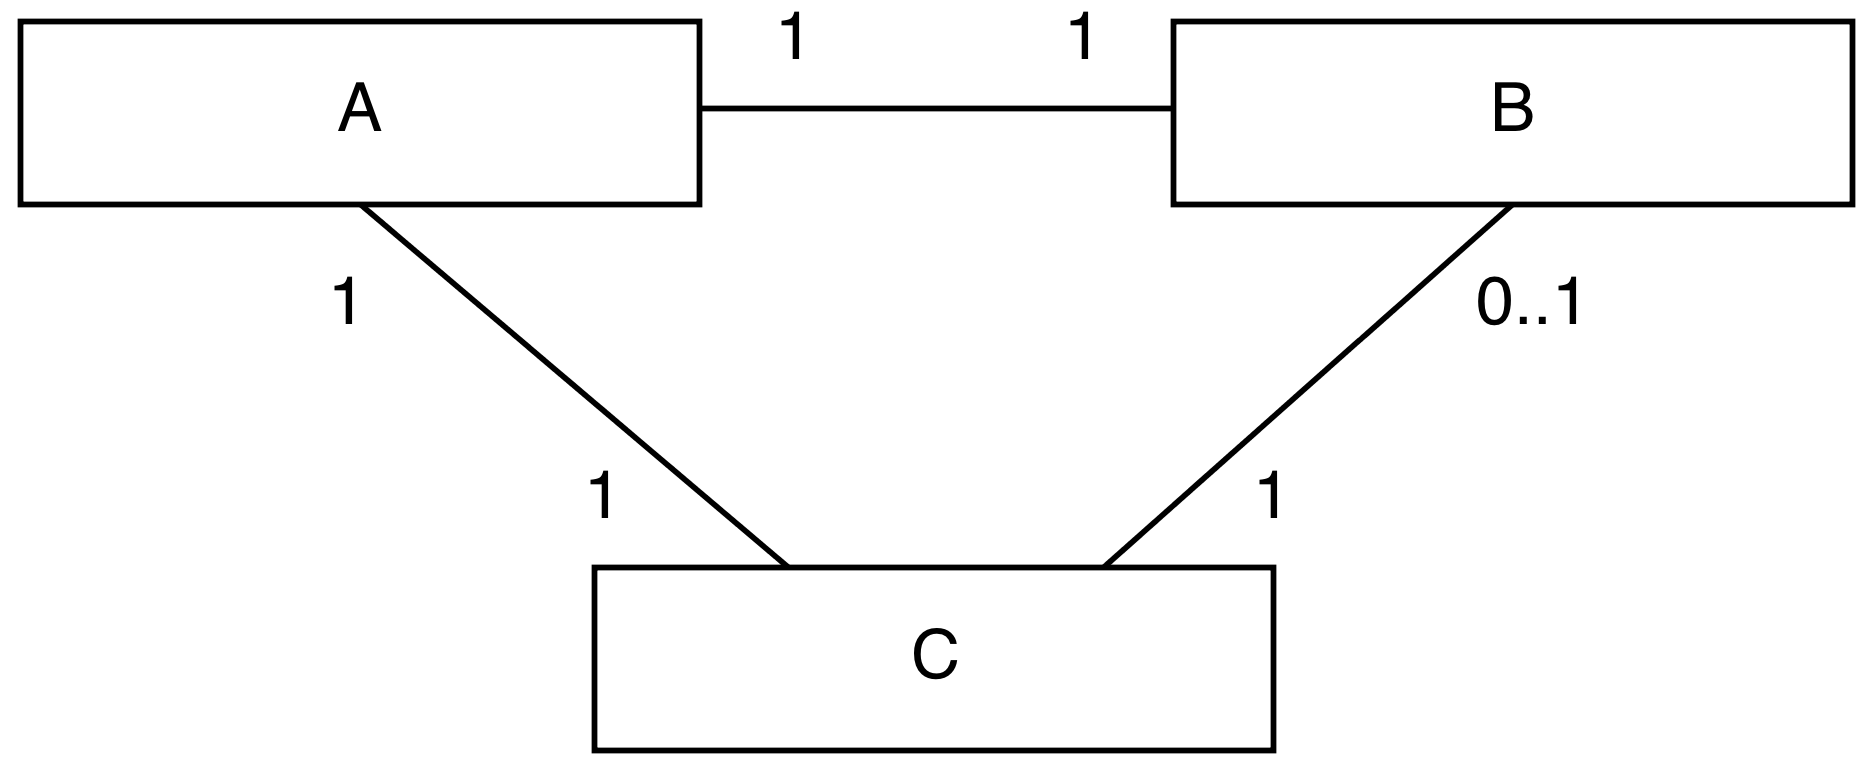
\includegraphics[width=0.55\textwidth]{images/generierung/infinite.png}
		\caption{Formal korrektes aber "`unerf�llbares"' Datenbankschema}\label{img:generierung:offen:infinite}
	\end{figure}

	Aus der Beschreibung geht schon hervor, dass es kein C geben kann, das nicht in Beziehung mit
	einer Entit�t aus B steht. Denn eine Entit�t in C muss mit einer Entit�t in A in Beziehung
	stehen, und eine Entit�t in A schlie�lich mit einer Entit�t in B. Und diese Entit�t in B
	ben�tigt eine Entit�t C f�r eine Beziehung. Es kommt entweder die Entit�t aus C in Frage,
	die nicht mit einer Entit�t aus B in Beziehung steht, oder es muss eine neue Entit�t in C
	generiert werden -- dann beginnt der Zyklus allerdings von vorne.
	
	Der Algorithmus w�rde sich hierbei immer f�r die zus�tzliche Generierung einer weiteren
	Entit�t in C entscheiden und schlie�lich nicht terminieren. Die momentane Implementierung bricht
	die Generierung allerdings nach �berschreiten eines Grenzwerts f�r nachtr�glich generierte
	Entit�ten ab.


  \chapter{Zusammenfassung und Ausblick}

\todo{Zusammenfassung und Fazit schreiben}

- Kurze Zusammenfassung: Was wurde erreicht

- Offene Punkte / Weiterführende Arbeiten
  %\chapter*{Titel}
\label{chap:titel}

\section*{Untertitel}
\label{Titel:�btertitel}


\subsection*{Stichpunkte}
\begin{itemize}
	\item
		\textbf{Item 1}: 
		Text

	\item
		\textbf{Item 2}: 
		Text
	
\end{itemize}


\subsection*{Aufz�hlung}
\begin{enumerate}
	\item
		\textbf{Item 1}: 
		Text

	\item
		\textbf{Item 2}: 
		Text
	
\end{enumerate}

\subsection*{Abk�rzung}
\nomenclature{GUI}{Graphical User Interface (Grafische Benutzeroberfl�che)}


\subsection*{Quellcode}
\begin{lstlisting}[caption=Der Titel, label=listing:label]
Code
\end{lstlisting}

\subsection*{Verweise}
\begin{enumerate}
	\item siehe \ref{listing:label}
	\item \reflst{listing:label}
	\item \refabb{img:imagelabel}
	\item \refsec{Titel:�btertitel}
	\item \refchap{chap:titel}
\end{enumerate}

\subsection*{Zitate}
\begin{enumerate}
	%\item \cite{MANUAL_ID}
	\item \cite{DSLS_IN_ACTION}
	\item \cite{REFACTORING_DATABASES}
	\item \cite{BASISWISSEN_SOFTWAETEST}
	\item \cite[20ff]{DER_INTEGRATIONSTEST}
	\item \cite{XUNIT_TEST_PATTERNS}
	\item \cite{DOMAIN_SPECIFIC_LANGUAGES}
	\item \cite{MODELLGETRIEBENE_SOFTWAREENTWICKLUNG}
\end{enumerate}

\subsection*{Bild}
\begin{figure}[H]
	\centering
	 
\includegraphics[width=0.8\textwidth]{images/cover/htwg_logo.png}
	\caption{Der Titel}\label{img:imagelabel}
\end{figure}


\subsection*{Bildgruppe}
\begin{figure}[htbp]
	\centering
	\subcaptionbox{Text 1\label{img:imagelabelX:image1}}[0.32\textwidth]{
		 
\includegraphics[width=0.32\textwidth]{images/cover/htwg_logo.png}
	}
	\subcaptionbox{Text 2\label{img:imagelabelX:image2}}[0.32\textwidth]{
		 
\includegraphics[width=0.25\textwidth]{images/cover/htwg_logo.png}
	}
	\subcaptionbox{Text 3\label{img:imagelabelX:image3}}[0.32\textwidth]{
		 
\includegraphics[width=0.16\textwidth]{images/cover/htwg_logo.png}
	}
	\caption{Gemeinsamer Titel}\label{img:imagelabelX}
\end{figure}




  
  %\phantomsection % n�tig damit das Tabellenverzeichnis korrekt verlinkt wird
  %\cleardoublepage
  %\printnomenclature
  %\addcontentsline{toc}{chapter}{Abk�rzungsverzeichnis}
  

  %% Abbildungsverzeichnis generieren
  \phantomsection  % n�tig damit das Abbildungsverzeichnis korrekt verlinkt wird
  \cleardoublepage
  \listoffigures
  \addcontentsline{toc}{chapter}{Abbildungsverzeichnis}
  
  %% Listingverzeichnis generieren
  \phantomsection  % n�tig damit das Listingverzeichnis korrekt verlinkt wird
  \cleardoublepage
  \lstlistoflistings
  \addcontentsline{toc}{chapter}{Listings}
  
  %% Tabellenverzeichnis generieren
  %\phantomsection % n�tig damit das Tabellenverzeichnis korrekt verlinkt wird
  %\cleardoublepage
  %\listoftables
  %\addcontentsline{toc}{chapter}{Tabellenverzeichnis}

  %% Literaturverzeichnis generieren
  \phantomsection  % n�tig damit das Literaturverzeichnis korrekt verlinkt wird
  \cleardoublepage
  \printbibliography  
  \addcontentsline{toc}{chapter}{Literaturverzeichnis}

  %% Abschnitt fuer den Anhang
  \begin{appendix}
	\chapter{Modell}
\label{chap:anhang:modell}

\lstSetTiny
\begin{lstlisting}[caption=Das verwendete Datenbank-Modell, label=listing:modell]
package model;

import com.seitenbau.testing.dbunit.generator.DataType;
import com.seitenbau.testing.dbunit.generator.DatabaseModel;
import com.seitenbau.testing.dbunit.generator.Table;
import com.seitenbau.testing.dbunit.generator.values.DateGenerator;
import com.seitenbau.testing.dbunit.generator.values.IntegerGenerator;
import com.seitenbau.testing.dbunit.generator.values.NachnameGenerator;
import com.seitenbau.testing.dbunit.generator.values.VornameGenerator;

public class HochschuleModel extends DatabaseModel
{
  public HochschuleModel()
  {
    database("Hochschule");
    packageName("com.seitenbau.testing.hochschule.model");
    enableTableModelClassesGeneration();
    seed(0);
    infinite(2);

    Table raum = table("raum")
        .description("Die Tabelle mit den R�umen der Hochschule")
        .seed(0)
        .minEntities(20)
        .column("id", DataType.BIGINT)
          .defaultIdentifier()
          .autoInvokeNext()
        .column("gebaude", DataType.VARCHAR)
        .column("nummer", DataType.VARCHAR)
      .build();

    Table professoren = table("professor")
        .description("Die Tabelle mit den Professoren der Hochschule")
        .column("id", DataType.BIGINT)
          .defaultIdentifier()
          .autoInvokeNext()
        .column("name", DataType.VARCHAR)
          .generator(new NachnameGenerator())
        .column("vorname", DataType.VARCHAR)
          .generator(new VornameGenerator())
        .column("titel", DataType.VARCHAR)
        .column("fakultaet", DataType.VARCHAR)
        .column("raum_id", DataType.BIGINT)
          .reference
            .local
              .name("hatRaum")
            .foreign(raum)
              .name("gehoert")
              .multiplicity("0..1")
      .build();

    Table lehrveranstaltungen = table("lehrveranstaltung")
        .description("Die Tabelle mit den Lehrveranstaltungen der Hochschule")
        .column("id", DataType.BIGINT)
          .defaultIdentifier()
          .autoInvokeNext()
        .column("professor_id", DataType.BIGINT)
          .reference
            .local
              .name("geleitetVon")
              .description("Gibt an, von welchem Professor eine Lehrveranstaltung geleitet wird.")
            .foreign(professoren)
              .name("leitet")
              .description("Gibt an, welche Lehrveranstaltungen ein Professor leitet.")
              .multiplicity("0..*")
        .column("name", DataType.VARCHAR)
        .column("sws", DataType.INTEGER)
          .generator(new IntegerGenerator(2, 6))
        .column("ects", DataType.DOUBLE)
      .build();

    Table pruefungen = table("pruefung")
        .description("Die Tabelle mit den Pr�fungen der Hochschule")
        .column("id", DataType.BIGINT)
          .defaultIdentifier()
          .autoInvokeNext()
        .column("lehrveranstaltung_id", DataType.BIGINT)
          .reference
            .local
              .name("stoffVon")
              .multiplicity("1")
              .description("Gibt an, zu welcher Lehrvanstaltung eine Pr�fung geh�rt.")
            .foreign(lehrveranstaltungen)
              .name("hatPruefung")
              .multiplicity("0..*")
              .description("Ordnet Pr�fungen einer Lehrveranstaltung zu.")
        .column("typ", DataType.VARCHAR)
        .column("zeitpunkt", DataType.DATE)
          .generator(new DateGenerator())
      .build();

    Table studenten = table("student")
        .description("Die Tabelle mit den immatrikulierten Studenten der Hochschule")
        .column("matrikelnummer", DataType.BIGINT)
          .defaultIdentifier()
          .autoInvokeNext()
        .column("name", DataType.VARCHAR)
          .generator(new NachnameGenerator())
        .column("vorname", DataType.VARCHAR)
          .generator(new VornameGenerator())
        .column("studiengang", DataType.VARCHAR)
        .column("semester", DataType.INTEGER)
          .generator(new IntegerGenerator(1, 8))
        .column("immatrikuliert_seit", DataType.DATE)
          .generator(new DateGenerator())
      .build();

    associativeTable("beaufsichtigt")
        .column("professor_id", DataType.BIGINT)
          .reference
            .foreign(professoren)
              .name("beaufsichtigt")
              .description("Gibt an, welche Pr�fungen ein Professor beaufsichtigt.")
              .multiplicity("0..*")
        .column("pruefung_id", DataType.BIGINT)
          .reference
            .foreign(pruefungen)
              .name("beaufsichtigtVon")
              .description("Gibt an, welche Professoren eine Pr�fung beaufsichtigen.")
              .multiplicity("0..*")
      .build();

    associativeTable("besucht")
        .column("student_id", DataType.BIGINT)
          .reference
            .foreign(studenten)
              .name("besucht")
              .multiplicity("0..*")
              .description("Gibt an, welche Lehrveranstaltungen ein Student besucht.")
        .column("lehrveranstaltung_id", DataType.BIGINT)
          .reference
            .foreign(lehrveranstaltungen)
              .name("besuchtVon")
              .multiplicity("3..10")
              .description("Gibt an, welche Studenten eine Lehrveranstaltung besuchen.")
      .build();

    associativeTable("isttutor")
        .column("student_id", DataType.BIGINT)
          .reference
            .foreign(studenten)
              .name("istTutor")
              .multiplicity("0..*")
              .description("Gibt an, bei welchen Lehrveranstaltungen ein Student Tutor ist.")
        .column("lehrveranstaltung_id", DataType.BIGINT)
          .reference
            .foreign(lehrveranstaltungen)
              .name("hatTutor")
              .multiplicity("0..*")
              .description("Gibt an, welche Tutoren eine Lehrveranstaltung hat.")
      .build();

    associativeTable("schreibt")
        .column("student_id", DataType.BIGINT)
          .reference
            .foreign(studenten)
              .name("schreibt")
              .multiplicity("0..*")
              .description("Gibt an, welche Pr�fungen ein Student schreibt.")
        .column("pruefung_id", DataType.BIGINT)
          .reference
            .foreign(pruefungen)
              .name("geschriebenVon")
              .multiplicity("0..*")
              .description("Gibt an, welche Studenten eine Pr�fung schreiben.")
        .column("versuch", DataType.INTEGER)
          .generator(new IntegerGenerator(1, 3))
      .build();
  }

}
\end{lstlisting}
\lstSetNormal

	\chapter{Generierte DSL}
\label{chap:anhang:generiertedsl}

\lstSetTiny
\begin{lstlisting}[caption=Generierte DSL, label=listing:generiertedsl]
package dataset

import com.seitenbau.testing.hochschule.model.*

class DataSet extends HochschuleBuilder
{

  def tables() {

    raumTable.rows() {
      REF     | gebaude | nummer
      RAUM_1  | "Delta" | "dolor"
      RAUM_2  | "Maus"  | "Lorem"
      RAUM_3  | "amet"  | "amet"
      RAUM_4  | "Delta" | "Lorem"
      RAUM_5  | "ipsum" | "Beta"
      RAUM_6  | "Katze" | "dolor"
      RAUM_7  | "Beta"  | "Alpha"
      RAUM_8  | "Hund"  | "Alpha"
      RAUM_9  | "Gamma" | "Lorem"
      RAUM_10 | "ipsum" | "Hund"
      RAUM_11 | "Maus"  | "amet"
      RAUM_12 | "amet"  | "Alpha"
      RAUM_13 | "amet"  | "amet"
    }

    professorTable.rows() {
      REF          | name         | vorname    | titel   | fakultaet | raum_id
      PROFESSOR_1  | "Fischer"    | "Thomas"   | "Katze" | "Maus"    | RAUM_2
      PROFESSOR_2  | "Fischer"    | "Stefan"   | "Delta" | "Beta"    | RAUM_3
      PROFESSOR_3  | "Fischer"    | "Claudia"  | "ipsum" | "amet"    | RAUM_4
      PROFESSOR_4  | "Schneider"  | "Angelika" | "sit"   | "Lorem"   | RAUM_5
      PROFESSOR_5  | "Schmidt"    | "Simone"   | "Lorem" | "Gamma"   | RAUM_6
      PROFESSOR_6  | "Meyer"      | "Brigitte" | "sit"   | "Maus"    | RAUM_7
      PROFESSOR_7  | "Fischer"    | "Bettina"  | "Gamma" | "amet"    | RAUM_8
      PROFESSOR_8  | "Schneider"  | "Thorsten" | "Lorem" | "ipsum"   | RAUM_9
      PROFESSOR_9  | "Mustermann" | "Markus"   | "ipsum" | "sit"     | RAUM_10
      PROFESSOR_10 | "M�ller"     | "Elke"     | "Lorem" | "Lorem"   | RAUM_11
      PROFESSOR_11 | "Mustermann" | "Heike"    | "ipsum" | "dolor"   | RAUM_12
      PROFESSOR_12 | "M�ller"     | "Markus"   | "sit"   | "amet"    | RAUM_13
    }

    raum2Table.rows() {
      REF      | professor_id
      RAUM2_1  | _
      RAUM2_2  | PROFESSOR_1
      RAUM2_3  | PROFESSOR_2
      RAUM2_4  | PROFESSOR_3
      RAUM2_5  | PROFESSOR_4
      RAUM2_6  | PROFESSOR_5
      RAUM2_7  | PROFESSOR_6
      RAUM2_8  | PROFESSOR_7
      RAUM2_9  | PROFESSOR_8
      RAUM2_10 | PROFESSOR_9
      RAUM2_11 | PROFESSOR_10
      RAUM2_12 | PROFESSOR_11
      RAUM2_13 | PROFESSOR_12
    }

    lehrveranstaltungTable.rows() {
      REF                  | professor_id | name    | sws | ects
      LEHRVERANSTALTUNG_1  | PROFESSOR_2  | "Alpha" | 6   | "amet"
      LEHRVERANSTALTUNG_2  | PROFESSOR_3  | "Hund"  | 2   | "Gamma"
      LEHRVERANSTALTUNG_3  | PROFESSOR_3  | "Katze" | 4   | "ipsum"
      LEHRVERANSTALTUNG_4  | PROFESSOR_3  | "dolor" | 6   | "Delta"
      LEHRVERANSTALTUNG_5  | PROFESSOR_3  | "Lorem" | 3   | "Beta"
      LEHRVERANSTALTUNG_6  | PROFESSOR_3  | "Gamma" | 6   | "Gamma"
      LEHRVERANSTALTUNG_7  | PROFESSOR_4  | "Gamma" | 5   | "Gamma"
      LEHRVERANSTALTUNG_8  | PROFESSOR_4  | "Alpha" | 5   | "dolor"
      LEHRVERANSTALTUNG_9  | PROFESSOR_4  | "sit"   | 4   | "sit"
      LEHRVERANSTALTUNG_10 | PROFESSOR_4  | "Delta" | 4   | "Katze"
      LEHRVERANSTALTUNG_11 | PROFESSOR_4  | "amet"  | 5   | "ipsum"
      LEHRVERANSTALTUNG_12 | PROFESSOR_4  | "sit"   | 4   | "Delta"
    }

    pruefungTable.rows() {
      REF         | lehrveranstaltung_id | typ     | zeitpunkt
      PRUEFUNG_1  | LEHRVERANSTALTUNG_2  | "sit"   | "12.01.1964"
      PRUEFUNG_2  | LEHRVERANSTALTUNG_3  | "Hund"  | "16.05.1911"
      PRUEFUNG_3  | LEHRVERANSTALTUNG_3  | "Delta" | "24.01.1971"
      PRUEFUNG_4  | LEHRVERANSTALTUNG_3  | "Lorem" | "29.06.1969"
      PRUEFUNG_5  | LEHRVERANSTALTUNG_3  | "Lorem" | "09.01.1958"
      PRUEFUNG_6  | LEHRVERANSTALTUNG_3  | "Alpha" | "12.01.1946"
      PRUEFUNG_7  | LEHRVERANSTALTUNG_4  | "Alpha" | "17.10.1944"
      PRUEFUNG_8  | LEHRVERANSTALTUNG_4  | "Alpha" | "02.06.2005"
      PRUEFUNG_9  | LEHRVERANSTALTUNG_4  | "Lorem" | "02.04.1986"
      PRUEFUNG_10 | LEHRVERANSTALTUNG_4  | "dolor" | "13.11.1921"
      PRUEFUNG_11 | LEHRVERANSTALTUNG_4  | "Alpha" | "15.12.2010"
      PRUEFUNG_12 | LEHRVERANSTALTUNG_4  | "ipsum" | "22.05.1939"
    }

    studentTable.rows() {
      REF        | name         | vorname    | studiengang | semester | immatrikuliert_seit
      STUDENT_1  | "Meyer"      | "Manuela"  | "Katze"     | 8        | "11.04.1952"
      STUDENT_2  | "Mustermann" | "Manuela"  | "Alpha"     | 3        | "09.09.1954"
      STUDENT_3  | "Fischer"    | "Brigitte" | "Lorem"     | 4        | "21.01.1901"
      STUDENT_4  | "Meyer"      | "Silke"    | "ipsum"     | 8        | "21.05.1945"
      STUDENT_5  | "M�ller"     | "Elke"     | "Alpha"     | 2        | "28.06.1939"
      STUDENT_6  | "Fischer"    | "Angelika" | "ipsum"     | 2        | "13.07.1955"
      STUDENT_7  | "Meyer"      | "Claudia"  | "Lorem"     | 1        | "01.04.1972"
      STUDENT_8  | "M�ller"     | "Stefan"   | "Beta"      | 3        | "06.06.1925"
      STUDENT_9  | "Meyer"      | "Angelika" | "ipsum"     | 2        | "20.03.2008"
      STUDENT_10 | "Meyer"      | "Silke"    | "Lorem"     | 3        | "25.05.1907"
      STUDENT_11 | "Fischer"    | "Stefan"   | "sit"       | 7        | "02.12.1984"
      STUDENT_12 | "Schneider"  | "Simone"   | "ipsum"     | 6        | "13.11.1972"
      STUDENT_13 | "Schneider"  | "Thomas"   | "Beta"      | 5        | "10.05.1945"
      STUDENT_14 | "Mustermann" | "Stefan"   | "Lorem"     | 4        | "19.02.1983"
      STUDENT_15 | "Fischer"    | "Brigitte" | "Alpha"     | 3        | "19.04.1953"
      STUDENT_16 | "Schneider"  | "Thorsten" | "Delta"     | 4        | "28.05.1989"
      STUDENT_17 | "Mustermann" | "Claudia"  | "Katze"     | 6        | "19.05.1915"
      STUDENT_18 | "Mustermann" | "Stefan"   | "Beta"      | 2        | "30.06.1934"
      STUDENT_19 | "Schneider"  | "Angelika" | "Delta"     | 4        | "09.08.1948"
      STUDENT_20 | "M�ller"     | "Bettina"  | "Hund"      | 4        | "16.11.1929"
      STUDENT_21 | "Schmidt"    | "Simone"   | "dolor"     | 8        | "03.08.1962"
      STUDENT_22 | "Fischer"    | "Thomas"   | "Lorem"     | 6        | "13.04.1939"
      STUDENT_23 | "Meyer"      | "Andreas"  | "Alpha"     | 7        | "17.02.1966"
      STUDENT_24 | "Fischer"    | "Brigitte" | "dolor"     | 2        | "06.12.1924"
      STUDENT_25 | "Schneider"  | "Markus"   | "sit"       | 8        | "28.09.1977"
      STUDENT_26 | "Schneider"  | "Claudia"  | "Lorem"     | 4        | "13.10.1927"
      STUDENT_27 | "Mustermann" | "Simone"   | "Maus"      | 8        | "27.02.1959"
      STUDENT_28 | "M�ller"     | "Bettina"  | "Alpha"     | 8        | "27.09.1952"
      STUDENT_29 | "Mustermann" | "Stefan"   | "Beta"      | 6        | "03.10.1987"
      STUDENT_30 | "Schmidt"    | "Thomas"   | "Katze"     | 2        | "19.05.1915"
      STUDENT_31 | "Meyer"      | "Stefan"   | "amet"      | 8        | "02.10.1937"
      STUDENT_32 | "Schmidt"    | "Claudia"  | "Delta"     | 7        | "25.10.1998"
      STUDENT_33 | "Schneider"  | "Heike"    | "amet"      | 7        | "22.12.1901"
      STUDENT_34 | "Mustermann" | "Elke"     | "Hund"      | 2        | "02.12.1984"
      STUDENT_35 | "Mustermann" | "Thomas"   | "Hund"      | 8        | "27.07.1950"
      STUDENT_36 | "Meyer"      | "Stefan"   | "amet"      | 7        | "19.03.1949"
      STUDENT_37 | "Meyer"      | "Heike"    | "Gamma"     | 1        | "18.09.1905"
      STUDENT_38 | "M�ller"     | "Heike"    | "sit"       | 6        | "23.08.1941"
      STUDENT_39 | "Mustermann" | "Brigitte" | "Delta"     | 2        | "08.09.1981"
      STUDENT_40 | "Meyer"      | "Bettina"  | "ipsum"     | 1        | "23.10.1915"
      STUDENT_41 | "Meyer"      | "Simone"   | "Hund"      | 6        | "07.03.1929"
      STUDENT_42 | "Meyer"      | "Thomas"   | "ipsum"     | 6        | "23.03.1973"
      STUDENT_43 | "Mustermann" | "Brigitte" | "Gamma"     | 4        | "15.10.1988"
      STUDENT_44 | "Schmidt"    | "Silke"    | "Katze"     | 2        | "22.11.1975"
      STUDENT_45 | "Schmidt"    | "Thomas"   | "Gamma"     | 4        | "17.07.1971"
      STUDENT_46 | "Fischer"    | "Manuela"  | "dolor"     | 4        | "15.06.1956"
      STUDENT_47 | "Schmidt"    | "Markus"   | "Beta"      | 6        | "27.05.1919"
      STUDENT_48 | "Schmidt"    | "Elke"     | "Alpha"     | 7        | "25.10.1952"
      STUDENT_49 | "M�ller"     | "Heike"    | "Beta"      | 6        | "07.01.1956"
      STUDENT_50 | "Schneider"  | "Thorsten" | "Lorem"     | 5        | "11.04.2002"
      STUDENT_51 | "Meyer"      | "Simone"   | "Beta"      | 2        | "31.12.1965"
      STUDENT_52 | "Mustermann" | "Bettina"  | "Hund"      | 4        | "15.06.1981"
    }

    beaufsichtigtTable.rows() {
      professor_id | pruefung_id
      PROFESSOR_1  | PRUEFUNG_1
      PROFESSOR_2  | PRUEFUNG_2
      PROFESSOR_2  | PRUEFUNG_3
      PROFESSOR_3  | PRUEFUNG_4
      PROFESSOR_4  | PRUEFUNG_4
      PROFESSOR_5  | PRUEFUNG_5
      PROFESSOR_5  | PRUEFUNG_6
      PROFESSOR_6  | PRUEFUNG_5
      PROFESSOR_6  | PRUEFUNG_6
      PROFESSOR_7  | PRUEFUNG_7
      PROFESSOR_8  | PRUEFUNG_8
      PROFESSOR_8  | PRUEFUNG_9
      PROFESSOR_9  | PRUEFUNG_10
      PROFESSOR_10 | PRUEFUNG_10
      PROFESSOR_11 | PRUEFUNG_11
      PROFESSOR_11 | PRUEFUNG_12
      PROFESSOR_12 | PRUEFUNG_11
      PROFESSOR_12 | PRUEFUNG_12
    }

    besuchtTable.rows() {
      student_id | lehrveranstaltung_id
      STUDENT_1  | LEHRVERANSTALTUNG_1
      STUDENT_2  | LEHRVERANSTALTUNG_1
      STUDENT_3  | LEHRVERANSTALTUNG_1
      STUDENT_4  | LEHRVERANSTALTUNG_2
      STUDENT_4  | LEHRVERANSTALTUNG_3
      STUDENT_5  | LEHRVERANSTALTUNG_2
      STUDENT_5  | LEHRVERANSTALTUNG_3
      STUDENT_6  | LEHRVERANSTALTUNG_2
      STUDENT_6  | LEHRVERANSTALTUNG_3
      STUDENT_7  | LEHRVERANSTALTUNG_4
      STUDENT_8  | LEHRVERANSTALTUNG_4
      STUDENT_9  | LEHRVERANSTALTUNG_4
      STUDENT_10 | LEHRVERANSTALTUNG_4
      STUDENT_11 | LEHRVERANSTALTUNG_4
      STUDENT_12 | LEHRVERANSTALTUNG_4
      STUDENT_13 | LEHRVERANSTALTUNG_4
      STUDENT_14 | LEHRVERANSTALTUNG_4
      STUDENT_15 | LEHRVERANSTALTUNG_4
      STUDENT_16 | LEHRVERANSTALTUNG_4
      STUDENT_17 | LEHRVERANSTALTUNG_5
      STUDENT_17 | LEHRVERANSTALTUNG_6
      STUDENT_18 | LEHRVERANSTALTUNG_5
      STUDENT_18 | LEHRVERANSTALTUNG_6
      STUDENT_19 | LEHRVERANSTALTUNG_5
      STUDENT_19 | LEHRVERANSTALTUNG_6
      STUDENT_20 | LEHRVERANSTALTUNG_5
      STUDENT_20 | LEHRVERANSTALTUNG_6
      STUDENT_21 | LEHRVERANSTALTUNG_5
      STUDENT_21 | LEHRVERANSTALTUNG_6
      STUDENT_22 | LEHRVERANSTALTUNG_5
      STUDENT_22 | LEHRVERANSTALTUNG_6
      STUDENT_23 | LEHRVERANSTALTUNG_5
      STUDENT_23 | LEHRVERANSTALTUNG_6
      STUDENT_24 | LEHRVERANSTALTUNG_5
      STUDENT_24 | LEHRVERANSTALTUNG_6
      STUDENT_25 | LEHRVERANSTALTUNG_5
      STUDENT_25 | LEHRVERANSTALTUNG_6
      STUDENT_26 | LEHRVERANSTALTUNG_5
      STUDENT_26 | LEHRVERANSTALTUNG_6
      STUDENT_27 | LEHRVERANSTALTUNG_7
      STUDENT_28 | LEHRVERANSTALTUNG_7
      STUDENT_29 | LEHRVERANSTALTUNG_7
      STUDENT_30 | LEHRVERANSTALTUNG_8
      STUDENT_30 | LEHRVERANSTALTUNG_9
      STUDENT_31 | LEHRVERANSTALTUNG_8
      STUDENT_31 | LEHRVERANSTALTUNG_9
      STUDENT_32 | LEHRVERANSTALTUNG_8
      STUDENT_32 | LEHRVERANSTALTUNG_9
      STUDENT_33 | LEHRVERANSTALTUNG_10
      STUDENT_34 | LEHRVERANSTALTUNG_10
      STUDENT_35 | LEHRVERANSTALTUNG_10
      STUDENT_36 | LEHRVERANSTALTUNG_10
      STUDENT_37 | LEHRVERANSTALTUNG_10
      STUDENT_38 | LEHRVERANSTALTUNG_10
      STUDENT_39 | LEHRVERANSTALTUNG_10
      STUDENT_40 | LEHRVERANSTALTUNG_10
      STUDENT_41 | LEHRVERANSTALTUNG_10
      STUDENT_42 | LEHRVERANSTALTUNG_10
      STUDENT_43 | LEHRVERANSTALTUNG_11
      STUDENT_43 | LEHRVERANSTALTUNG_12
      STUDENT_44 | LEHRVERANSTALTUNG_11
      STUDENT_44 | LEHRVERANSTALTUNG_12
      STUDENT_45 | LEHRVERANSTALTUNG_11
      STUDENT_45 | LEHRVERANSTALTUNG_12
      STUDENT_46 | LEHRVERANSTALTUNG_11
      STUDENT_46 | LEHRVERANSTALTUNG_12
      STUDENT_47 | LEHRVERANSTALTUNG_11
      STUDENT_47 | LEHRVERANSTALTUNG_12
      STUDENT_48 | LEHRVERANSTALTUNG_11
      STUDENT_48 | LEHRVERANSTALTUNG_12
      STUDENT_49 | LEHRVERANSTALTUNG_11
      STUDENT_49 | LEHRVERANSTALTUNG_12
      STUDENT_50 | LEHRVERANSTALTUNG_11
      STUDENT_50 | LEHRVERANSTALTUNG_12
      STUDENT_51 | LEHRVERANSTALTUNG_11
      STUDENT_51 | LEHRVERANSTALTUNG_12
      STUDENT_52 | LEHRVERANSTALTUNG_11
      STUDENT_52 | LEHRVERANSTALTUNG_12
    }

    isttutorTable.rows() {
      student_id | lehrveranstaltung_id
      STUDENT_1  | LEHRVERANSTALTUNG_1
      STUDENT_2  | LEHRVERANSTALTUNG_2
      STUDENT_2  | LEHRVERANSTALTUNG_3
      STUDENT_3  | LEHRVERANSTALTUNG_4
      STUDENT_4  | LEHRVERANSTALTUNG_4
      STUDENT_5  | LEHRVERANSTALTUNG_5
      STUDENT_5  | LEHRVERANSTALTUNG_6
      STUDENT_6  | LEHRVERANSTALTUNG_5
      STUDENT_6  | LEHRVERANSTALTUNG_6
      STUDENT_7  | LEHRVERANSTALTUNG_7
      STUDENT_8  | LEHRVERANSTALTUNG_8
      STUDENT_8  | LEHRVERANSTALTUNG_9
      STUDENT_9  | LEHRVERANSTALTUNG_10
      STUDENT_10 | LEHRVERANSTALTUNG_10
      STUDENT_11 | LEHRVERANSTALTUNG_11
      STUDENT_11 | LEHRVERANSTALTUNG_12
      STUDENT_12 | LEHRVERANSTALTUNG_11
      STUDENT_12 | LEHRVERANSTALTUNG_12
    }

    schreibtTable.rows() {
      student_id | pruefung_id | versuch
      STUDENT_1  | PRUEFUNG_1  | 2
      STUDENT_2  | PRUEFUNG_2  | 2
      STUDENT_2  | PRUEFUNG_3  | 1
      STUDENT_3  | PRUEFUNG_4  | 2
      STUDENT_4  | PRUEFUNG_4  | 3
      STUDENT_5  | PRUEFUNG_5  | 1
      STUDENT_5  | PRUEFUNG_6  | 2
      STUDENT_6  | PRUEFUNG_5  | 3
      STUDENT_6  | PRUEFUNG_6  | 2
      STUDENT_7  | PRUEFUNG_7  | 3
      STUDENT_8  | PRUEFUNG_8  | 3
      STUDENT_8  | PRUEFUNG_9  | 1
      STUDENT_9  | PRUEFUNG_10 | 2
      STUDENT_10 | PRUEFUNG_10 | 3
      STUDENT_11 | PRUEFUNG_11 | 3
      STUDENT_11 | PRUEFUNG_12 | 2
      STUDENT_12 | PRUEFUNG_11 | 2
      STUDENT_12 | PRUEFUNG_12 | 3
    }

  }

}
\end{lstlisting}
\lstSetNormal

beaufsichtigt:	18
besucht:	78
isttutor:	18
lehrveranstaltung:	12
professor:	12
pruefung:	12
raum:	13
raum2:	13
schreibt:	18
student:	52

  \end{appendix}
	
	\todos
\end{document}